\documentclass[a4paper, 12pt, oneside]{report}
\usepackage[utf8]{inputenc}
\usepackage[english,french]{babel}

\usepackage{arabtex}
\usepackage{utf8}
\setcode{utf8}

\usepackage[left=2.00cm, right=2.cm, top=2.00cm, bottom=3.00cm]{geometry}
\usepackage[Lenny]{fncychap}
\usepackage{fancybox}
\usepackage{fancyhdr}
\usepackage{enumerate}
\usepackage[T1]{fontenc}
\usepackage{enumitem}
\usepackage{outlines}
\usepackage{mdframed}

\usepackage{rotating}
\usepackage{amsmath}
\usepackage{graphicx}
\usepackage{float}
\graphicspath{ {./img/} }
\usepackage{subfig}
\usepackage{tabularx}
\usepackage{hyperref}
\usepackage{url}

\newtheorem{proposition}{Proposition}[chapter]
\newtheorem{theorem}{Théorème}[chapter]
\newtheorem{corollaire}[proposition]{Corollaire}
\newtheorem{lemme}[proposition]{Lemme}
\newtheorem{definition}{Définition}[chapter]
\newtheorem{remarque}{Remarque}[chapter]
\newtheorem{exemple}{Exemple}[chapter]
\newtheorem{propriete}{Propriété}[chapter]

\newenvironment{proof}[1][Preuve]{\textbf{#1}}
{\ \rule{0.5em}{0.5em}}
\def\baselinestretch{1.5}
\pagestyle{fancy}
\fancyhead[L]{\slshape\rightmark}
\fancyhf{} 
\fancyfoot[C]{\thepage} 
\fancyhead[L]{\leftmark}
\fancypagestyle{plain}{%
    \fancyhead{}%
    \renewcommand{\headrulewidth}{0pt}
}
\headsep=13mm


\begin{document}
\setcounter{page}{1}
\pagenumbering{roman}

\thispagestyle{empty}
%++++++++++++++++++++++++++++++++++++++ 
\begin{arabtex}
\par\noindent
\small
\begin{center}
الجمهورية الجزائرية الديمقراطية الشعبية \\ وزارة التعليم العالي والبحث العلمي  
\end{center}
\end{arabtex}
%++++++++++++++++++++++++++++++++++++++ 
\selectlanguage{french}
\begin{center}
	\textbf{People’s Democratic Republic of Algeria} \\
	\textbf{Ministry of Higher Education and Scientific Research} \\
	\textbf{University of Algiers 1 Benyoucef BENKHEDDA}\\

	
\includegraphics[scale=0.3]{logo.jpg}\\

	\textbf{Faculté des Sciences} \\
	\textbf{Département d'Informatique}\\
	\textbf{Mémoire de fin d’études pour l’obtention du diplôme de\\ Master en Informatique} \\
	\textbf{Spécialité : Ingénierie des Systèmes Informatiques Intelligents}\\

	
	\textbf{{\large{Thème}}}
	\vspace{0.125cm}\noindent
	\rule{\textwidth}{2pt} 
	\Large\bf{Un système temps-réel et intelligent pour la gestion de parking} 
\end{center}
\noindent
  \rule{\textwidth}{2pt}
\vspace{0.1cm}
\par
\begin{center}
\textbf{Présenté et soutenu par :} \\
	\textbf{M. LOUNIS Amar}\\
	\textbf{M. MEDJBER Hamza}
	\vspace{0.5cm}
	\par
 \end{center}
{\bf Soutenu le 20 Septembre 2023 devant le jury composé de : } 
\begin{center}
\vspace{0.1cm}
	\begin{tabular}{lll}
		\bf M.  DJOUADI Yassine & Président &  Professeur à l'Université d'Alger 1   \\
		\bf Mme BOUFEDJI Dounia & Examinatrice & Docteur à l'Université d'Alger 1    \\
        \bf Mme BELATTAR Khadidja & Encadrante & Docteur à l'Université d'Alger 1   \\
	\end{tabular}


\vspace{2.0 cm}
\par

\end{center}
\begin{center}
\textbf{\Large{\emph{Remerciements}}}\\
\end{center}

\par
Nous souhaitons tout d'abord exprimer notre gratitude envers ALLAH pour nous avoir accordé la force, la patience et la détermination nécessaires pour mener à bien ce modeste projet, fruit de plusieurs années de dévouement.

\par
Nous tenons à exprimer notre profonde reconnaissance et nos sincères remerciements à notre promotrice, le Dr. BELATTAR Khadidja, pour son précieux soutien, ses orientations et le temps qu'elle a généreusement consacré à notre encadrement.

\par
Nous exprimons également notre gratitude envers les membres du jury, à savoir Pr. DJOUADI Yassine et Dr. BOUFEDJI Dounia, qui nous ont honorés en examinant notre travail.

\par
Nous souhaitons également remercier chaleureusement chacun de nos enseignants à l'université d'Alger 1 - Benyoucef Benkhedda, pour la qualité de l'enseignement qu'ils nous ont dispensé au cours de notre cursus universtaire.

\par
Nous tenons à remercier sincèrement Mlle KOURI Ferial  et toutes les personnes qui ont contribué de près ou de loin à notre réussite.
\\

%------------------------------------------------- 1 Dédicaces
\begin{center}
\textbf{\Large{\emph{Dédicaces}}}\\
\end{center}
\paragraph{}
\par
Je dédie ce travail à mes chers parents qui m'ont accompagné dans leurs prières tout au long de mon parcours universitaire.
\par
À ma chère épouse, ma compagne de vie, à ma fille Nihal, la première joie de paternité de ma vie.
\par
À mes chers frères et sœurs.
\par
À mon binôme MEDJBER Hamza qui a partagé ce travail avec moi.
\par
À toute personne qui m'a aidé pour continuer ce travail.

\begin{flushright}
\textit{\textbf{LOUNIS Amar.}}
\end{flushright}

%------------------------------------------------- 2 Dédicaces
\newpage

\begin{center}
\textbf{\Large{\emph{Dédicaces}}}\\
\end{center}
\paragraph{}
\par
Je dédie ce travail  à mon cher père qui m'a soutenu tout au long de mon parcours académique,
\par
À  ma chère mère qui m'a accompagné dans ses prières et ses douaas tout au long de mon parcours académique, 
\par
À mes chers frères et sœurs.
\par
À mes  nièces  et mes neveux.
\par
À mon binôme LOUNIS Amar, qui a partagé ce travail avec moi.
\begin{flushright}
\textit{\textbf{MEDJBER Hamza.}}
\end{flushright}
\begin{RLtext}
\par
\textbf{\Large{ملخص}}\\
\small

مع النمو الكبير في عدد السيارات حول العالم أصبح الطلب المتزايد على مواقف السيارات في المدن الكبيرة أمرًا ضروريًا نظرًا لندرة هذه المساحات ووجود أساليب الإدارة التقليدية  هذا الوضع يستدعي اعتماد تكنولوجيات جديدة لإدارة مواقف السيارات بطريقة ذكية  مما يضمن التنظيم الفعّال والاستفادة الأمثل من هذه الموارد  الهدف الرئيسي هو الاستفادة الكاملة من المساحة المخصصة  واستيعاب المزيد من السيارات  وضمان راحة السائقين، وتقليل ازدحام حركة المرور 
\par
الإدارة التقليدية لمواقف السيارات عادةً ما تتضمن تسجيل أوقات دخول وخروج السيارات مع لوحات تراخيصها مع الحفاظ على تتبع دقيق للمساحات المتاحة  يتم تكليف مهام هذه المسؤوليات عادة لموظف استقبال يستقبل 
السيارات عند وصولها، ويفحص لوحات التراخيص، ويسجل المعلومات اللازمة 


\par
في هذا السياق، يركز عملنا على تطوير نظام ذكي لإدارة مواقف السيارات إعتمادا على الذكاء الاصطناعي. يمكن لهذا النظام الآلي التعرف على السيارات في حالة الحركة أو الوقوف، واكتشاف وقراءة لوحات التراخيص، وحساب عدد  المساحات المتاحة والمحتلة، دون تدخل بشري. باستخدام النموذج \LR{YOLOv8}، اختبرنا هذا الحل باستخدام صور للسيارات الجزائرية ولوحات تراخيصها التي تم جمعها من مصادر مثل \LR{Ouedkniss}  و \LR{Facebook}.  ثم قمنا بتقييم أداء النظام من خلال مقارنته مع  النمودجين \LR{SSD} و \LR{Faster RCNN}. أظهرت النتائج المحصل عليها أنها واعدة.


\textbf{الكلمات المفتاحية \LR{:}} 
 نظام الوقت الحقيقي ، إدارة مواقف السيارات، الكشف عن المركبات ، التعرف على لوحة الترخيص ، قراءة لوحة الترخيص ،  تتبع المركبات, \LR{YOLOV8} , \LR{SSD} , \LR{FASTER R-CNN} .
\end{RLtext}

\vspace{0.5cm}

\par
\textbf{\Large{Abstract}}\\

With the significant growth in the number of vehicles worldwide, the increasing demand for parking in metropolises has become imperative due to the scarcity of these spaces and the presence of traditional management methods. This situation necessitates the adoption of new technologies for intelligent parking management, ensuring efficient organization and optimal utilization of these resources. The primary goal is to fully exploit the dedicated parking space, accommodate more vehicles, ensure driver comfort, and reduce traffic congestion.

Conventional parking management typically involves recording vehicle entry and exit times along with their license plates while maintaining precise tracking of available spaces. These responsibilities are usually assigned to an attendant who receives vehicles upon arrival, checks license plates, and records the necessary information.

In this context, our work focuses on developing an intelligent parking management system based on artificial intelligence. This automated system can recognize vehicles in motion or stationary, it can also detect and read license plates, and calculate the number of available and occupied parking spaces, all without human intervention. Using the YLOLOv8 model, we tested this solution using images of Algerian vehicles and license plates collected from sources such as Ouedkniss and Facebook. We subsequently assessed the system's performance by comparing it to Faster RCNN and SSD detectors. The results obtained proved to be promising.


\textbf{Keywords}: Real-time system, parking management, vehicle detection, license plate recognition, vehicle tracking and object detector.

\vspace{0.5cm}

\par
\textbf{\Large{Résumé}}\\

Avec la croissance significative du nombre de véhicules dans le monde, l'augmentation de la demande de stationnement dans les métropoles s'impose en raison de la rareté de ces espaces et des méthodes de gestion traditionnelles en place. Cette situation nécessite l'adoption de nouvelles technologies pour une gestion intelligente des parkings, assurant ainsi une organisation efficace et une utilisation optimale de ces ressources. L'objectif principal est d'exploiter pleinement l'espace dédié au stationnement, d'accueillir davantage de véhicules, de garantir le confort des conducteurs et de réduire la congestion routière.
\par

La gestion du stationnement conventionnelle implique généralement l'enregistrement des heures d'entrée et de sortie des véhicules ainsi que de leurs plaques d'immatriculation, tout en assurant un suivi précis des places disponibles. Ces responsabilités sont habituellement dévolues à un agent qui se charge de recevoir les véhicules à leur arrivée, de vérifier les plaques d'immatriculation et de saisir les informations nécessaires.

\par

Dans ce contexte, notre mémoire se concentre sur le développement d'un système de gestion de stationnement intelligent basé sur l'intelligence artificielle. Ce système automatisé est capable de reconnaître les véhicules en mouvement ou à l'arrêt, de détecter les plaques d'immatriculation et de calculer le nombre de places disponibles et occupées dans les parkings, le tout sans intervention humaine. En utilisant le modèle Yolov8, nous avons expérimenté cette solution en utilisant des images de véhicules et de plaques d'immatriculation d'origine Algérienne que nous avons collectées à partir de sources telles qu'Ouedkniss et Facebook. Nous avons ensuite évalué les performances de ce système en le comparant avec les détecteurs Faster RCNN et SSD. Les résultats obtenus se sont avérés prometteurs.

\par \textbf{Mots-clés} : Système temps-réel, gestion du stationnement, détection de véhicules, reconnaissance de plaque d'immatriculation, suivi de véhicules, détecteur d'objets.

%\textbf{\Large{Résumé}}\\
% essayer de faire le résumé en Arabe et en Anglais
%\par
%La gestion de parking intelligente transforme les approches classiques grâce à l'incorporation de technologies avancées. Son but est d'optimiser l'usage des places de stationnement pour une expérience aisée des conducteurs, en automatisant le suivi des véhicules, l'attribution d'emplacements, la gestion des paiements et la sécurité. L'objectif est de diminuer les embouteillages, faciliter le stationnement, augmenter la satisfaction des clients et maximiser l'utilisation de l'espace disponible. 
%\par
%Habituellement, la gestion de parking requiert l'enregistrement des heures d'entrée/sortie des véhicules et de leurs plaques d'immatriculation, avec un calcul précis des places disponibles. L'ensemble de ces tâches sont effectuées par un employé spécialisé qui se concentre sur l'accueil des véhicules à leur arrivée, la vérification des autorisations et l'enregistrement des informations.
%\par
%Dans ce contexte, notre travail consiste à développer un système intelligent en temps-réel  pour la gestion de parking en utilisant de l’intelligence artificielle. Ce système automatisé l’identification des véhicules, suit leurs mouvements, détecte les plaques d’immatriculation et calcule le nombre de places disponibles et vacantes dans le parking sans intervention humaine. En utilisant le modèle YOLOv8, nous avons testé cette solution avec des images de voitures et de plaques d'immatriculation Algériennes collectées de Ouedkniss et Facebook, montrant ses performances face à EasyOCR et OpenALPR.

%\textbf{Mots clés: } Gestion de parking, système en temps réel, détection de véhicules, reconnaissance de plaques d'immatriculation, intelligence artificielle.

%La bonne gestion des parkings nécessite d'enregistrer l'heure d'entrée et de sortie de la voiture avec l'enregistrement de sa plaque d'immatriculation et vous devez connaître le nombre de places disponibles et ces opérations sont généralement effectuées par un employé spécialisé avec l'aide de quelques outils et programmes
%Le rôle de l'employé est généralement lorsqu'un véhicule arrive au stationnement .
%\begin{itemize}
 %   \item Connaître le nombre de places vides.
 %   \item Enregistrement d'une plaque d'immatriculation.
  %  \item Déterminez si le véhicule est autorisé à entrer.
%    \item Notez l'heure de son entrée.
%\end{itemize}
%Lorsque la voiture quitte le parking, l'employé Calcul de la durée de stationnement.\\
%\par
%La vision par ordinateur en temps réel est un domaine de recherche en informatique qui vise à permettre aux ordinateurs de comprendre et d’interpréter les images et les vidéos en temps réel. Cependant, il y a plusieurs défis à relever pour que cela soit possible. Par exemple, la vision par ordinateur doit être capable de traiter des images en temps réel, ce qui nécessite des algorithmes de traitement d’image très rapides et efficaces. De plus, la vision par ordinateur doit être capable de traiter des images dans des conditions difficiles, telles que des environnements peu éclairés ou des images floues. Enfin, la vision par ordinateur doit être capable de traiter des images dans des contextes complexes, tels que des scènes avec plusieurs objets en mouvement.\cite{lebigdata_01} \cite{ibm_01}\\
%\par
%Dans ce mémorandum, nous souhaitons concevoir et mettre en œuvre un système capable d'effectuer les tâches des employés et de faire en sorte que le processus de stationnement se déroule de manière automatique, à l'aide de la vision par ordinateur en temps réel et de l'intelligence artificielle, en créant un apprentissage en profondeur modèles capables de reconnaître les véhicules, les plaques d'immatriculation et les mouvements des véhicules.

%\textbf{Mots clés :} gestion des parkings, temps réel, vision par ordinateur , l'intelligence artificielle , apprentissage en profondeur ,reconnaître les véhicules , reconnaître les plaques d'immatriculation  .

\let\cleardoublepage\clearpage

\newpage
\markboth{Table des matières}{}
\addcontentsline{toc}{chapter}{Table des matières}
\tableofcontents

\newpage
\markboth{Table des figures}{}
\addcontentsline{toc}{chapter}{Table des figures}
\listoffigures

\newpage
\markboth{Liste des tableaux}{}
\addcontentsline{toc}{chapter}{Liste des tableaux}
\listoftables

\chapter*{Liste des abréviations}
\markboth{Liste des abréviations}{}
\addcontentsline{toc}{chapter}{Liste des abréviations}

\begin{tabular}{llll}

\textbf{OCR} & & & Optical Character Recognition\\
\textbf{API} & & & Application Programming Interface\\
\textbf{CNN} & & & Convolutional Neural Network\\
\textbf{ML} & & & Machine Learning\\
\textbf{UI} & & & User Interface\\
\textbf{DL} & & & Deep Learning.\\
\textbf{IA} & & & Intelligence Artificielle\\
\textbf{DNN} & & & Deep Neural Network\\
\textbf{MLP} & & & Multi-Layer Perceptron\\
\textbf{RNN} & & & Recurrent Neural Network\\
\textbf{SSD} & & & Single Shot MultiBox Detector\\
\textbf{YOLO} & & & You Only Look Once \\
\textbf{mAP} & & & Mean Average Precision \\
\textbf{NMS} & & & Non-Maximum Suppression  \\
\textbf{CV} & & & Computer Vision\\
\textbf{SGD} & & & Stochastic Gradient Descent\\
\textbf{VP} & & & Vrais Positifs\\
\textbf{VN} & & & Vrais Négatifs \\
\textbf{FP} & & & Faux Positifs\\
\textbf{FN} & & & Faux Négatifs \\
\textbf{HOG} & & & Histogrammes Orientés Gradients\\

\end{tabular}

\setcounter{page}{1}
\pagenumbering{arabic}

\chapter*{Introduction générale}
\markboth{Introduction générale}{}
\addcontentsline{toc}{chapter}{Introduction générale}
\thispagestyle{plain}

\section*{Contexte générale}
\addcontentsline{toc}{section}{Contexte générale}

Les parkings ont vu le jour à la fin du 19e siècle avec l'introduction des premières automobiles dans les villes du monde. Au départ, peu d'emplacements de stationnement spécifiques étaient nécessaires en raison du faible nombre de voitures, et les gens se garaient sur les bords de route ou dans des garages privés. Cependant, à mesure que le nombre de voitures augmentait et que les villes s'étendaient, le stationnement est devenu un enjeu crucial.

\section*{Problématique et motivation}
\addcontentsline{toc}{section}{Problématique et motivation}

La problématique qui se pose est la suivante : Comment optimiser la gestion des parkings pour répondre à la demande croissante de stationnement tout en minimisant les problèmes liés à la congestion, à la disponibilité limitée d'espace et à l'impact environnemental ? Cette question est motivée par la nécessité de relever ces défis complexes dans un contexte urbain en constante évolution. Les parkings jouent un rôle crucial dans la mobilité urbaine, l'accès aux services et le confort des citoyens, ce qui rend essentielle l'amélioration de leur gestion. Par conséquent, il est impératif de développer des solutions innovantes pour améliorer la gestion des parkings, en tirant parti des avancées technologiques récentes telles que l'intelligence artificielle.

\section*{Contribution}
\addcontentsline{toc}{section}{Contribution}

La contribution essentielle de ce travail réside dans le développement d'un système de gestion de stationnement en temps réel, basé sur le modèle YOLOv8. Ce système automatisé est capable de reconnaître les véhicules en mouvement ou à l'arrêt, de détecter les plaques d'immatriculation, et de calculer les places de stationnement disponibles et occupées, le tout sans nécessiter d'intervention humaine.

En outre, nous avons constitué une base de données réelle comprenant des images de véhicules et de plaques d'immatriculation Algériennes.

\section*{Plan du mémoire}
\addcontentsline{toc}{section}{Plan du mémoire}
Ce manuscrit se structure autour de quatre chapitres fondamentaux, à savoir :

\paragraph{Chapitre 1 :}
Gestion du stationnement.\\
 Dans le premier chapitre, nous explorons le contexte général de la gestion des parkings.

\paragraph{Chapitre 2 :}
Apprentissage profond et détection d'objet: Concepts et algorithmes.\\
Dans le second chapitre, nous abordons particulièrement le concept de l'apprentissage profond et ses divers paradigmes, ainsi que les principaux algorithmes liés à la détection d'objets dans ce domaine.

\paragraph{Chapitre 3 :}
Gestion automatisée du stationnement: État de l'art.\\
Dans le troisième chapitre, nous évoquons les principales caractéristiques des plaques d'immatriculation des voitures algériennes. Nous passons également en revue les approches employées pour la détection des véhicules, la reconnaissance des plaques d'immatriculation, l'identification des caractères numériques sur les plaques, ainsi que le suivi en temps -réel des véhicules.

\paragraph{Chapitre 4 :}
Système intelligent de gestion du parking: Réalisation, résultats et analyse.\\
Le quatrième chapitre est consacré à la présentation de la solution proposée et des résultats obtenus par le système de gestion de parking intelligent à base du modèle YOLOv8.
\chapter{Gestion du stationnement}
\markboth{Gestion du stationnement}{}
\section{Introduction}

La mise en œuvre d'une bonne gestion du stationnement est primordiale pour réduire les embouteillages, minimiser le temps de recherche de stationnement, favoriser la sécurité routière ainsi que contribuer à la création d’un environnement urbain plus fluide et confortable pour les citoyens.

Dans ce contexte, le premier chapitre explore le contexte générale de la gestion des parkings. Pour ce faire, nous avons commencé à définir le parking puis présenter les différents types de parking. Après cela, nous avons décrit les composants de base d’un système de gestion automatique de parking, ainsi que les meilleures pratiques en matière de gestion du parking. A la fin, nous avons effectué une étude de l’existant des zones de parking à Alger.


\section{Parking}
Étant donné que notre objectif est de réaliser un système de gestion du stationnement en temps réel, ce chapitre portera sur les bases du parking .

Le parking, également appelé parc de stationnement, est une zone spécialement conçue pour permettre aux véhicules de stationner, de manière temporaire ou prolongée. Il peut être public ou privé, situé en intérieur ou en extérieur. On peut trouver des parkings dans différents endroits tels que les aéroports, les hôpitaux, les bâtiments et les grands marchés, entre autres. Quant à la tarification, il peut être gratuit ou payant, selon les politiques de gestion mise en place \cite{parking}.\\
Le parking est souvent aménagé pour offrir une circulation fluide et sécurisée pour les véhicules. Il peut inclure également des services supplémentaires tels que la surveillance, le nettoyage de la voiture, le lavage et bien d'autres encore. Ces facilités visent à rendre le stationnement plus pratique et confortable pour les utilisateurs.
Son objectif est de répondre aux besoins de stationnement des conducteurs de véhicules dans les zones à forte densité de population et de trafic \cite{blog-direct-signaletique}.

une bonne gestion du parking contribue à une planification urbaine efficace, à la réduction de la congestion, à la promotion de la mobilité durable, à l'amélioration de la qualité de vie et à la gestion judicieuse des ressources financières.

\section{Types de parkings }

Les parkings peuvent être classés en plusieurs types en fonction de leurs caractéristiques (architecture du  parc, mode de paiement, accessibilité au parking, et la manière de stationnement) et de leurs utilisations \cite{evo-park}.

\subsection{Selon l'architecture  } 
Les parcs de stationnement les plus courants sont :
\begin{outline}
\1 \textbf{ Parcs de stationnement en surface:} sont les parkings les plus simples, situés généralement au niveau du sol. Ils peuvent être revêtus d'asphalte ou de béton et ne possèdent pas de structures ni de toits. Vous les trouvez fréquemment dans les centres commerciaux, les écoles et d'autres lieux publics, comme illustré dans la figure ci-dessous \ref{Surfacepark}.

\begin{figure}[H]
	\centering
	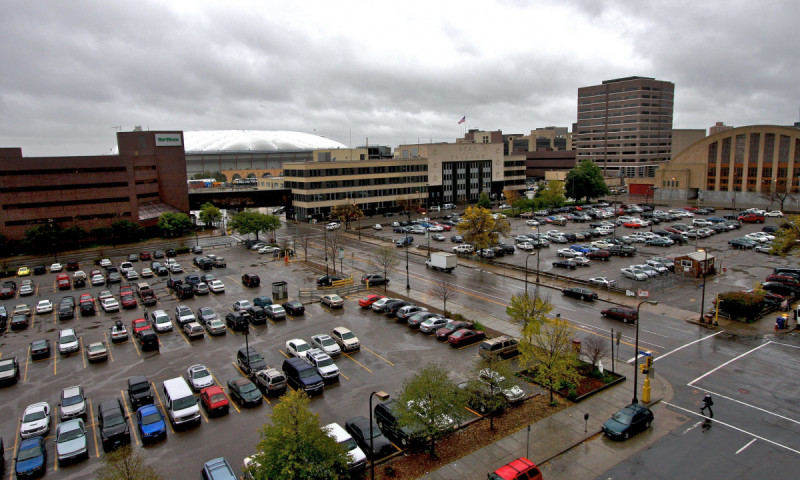
\includegraphics[height=05cm]{img/ch1-Surface parking-01.jpg}
	\caption{Parc de stationnement en surface}
 \label{Surfacepark}
\end{figure}

\1 \textbf{ Parcs de stationnement à étages: } Les parcs de stationnement à étages sont des structures qui ont plusieurs niveaux pour garer les voitures. Ils sont souvent faits de béton ou d'acier et ont des rampes ou des ascenseurs pour monter ou descendre entre les niveaux. Ces parkings peuvent être gérés automatiquement ou manuellement, et ils peuvent être couverts ou en plein air. Vous les trouvez souvent en ville, comme le montre l'image ci-dessous.. \ref{storeypark}.

\begin{figure}[H]
	\centering
	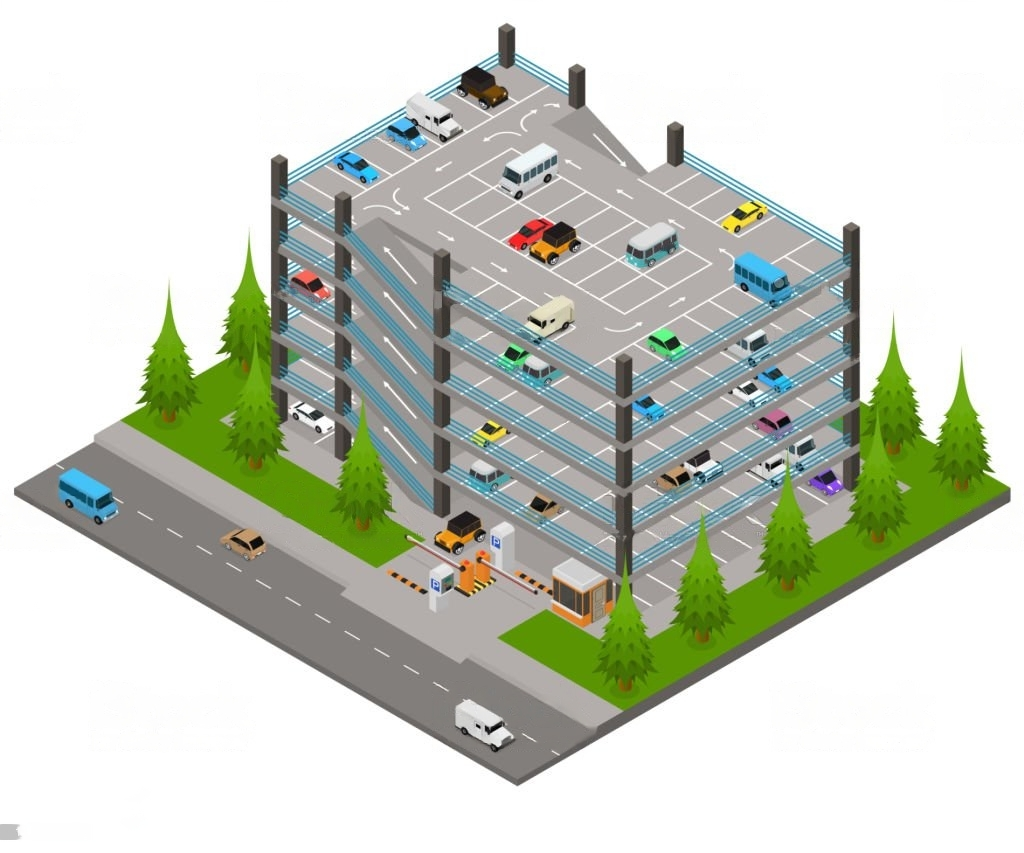
\includegraphics[height=06.5cm]{img/ch1-Multi-storey parking garages-01.jpeg}
	\caption{Parc de stationnement à étages}
 \label{storeypark}
 \end{figure}


%\textcolor{red}{}
\1 \textbf{Parcs de stationnement souterrains: } il s'agit de structures de stationnement situées sous le niveau du sol. Ils sont généralement accessibles par des rampes ou des ascenseurs et sont souvent utilisés dans des zones fortement peuplées où l'espace est limité. Ces parkings sont souvent gérés par des opérateurs et peuvent être équipés de systèmes de sécurité et des systèmes d'aération avec de nombreuses ventilations \cite{yespark-lexique}. Ils peuvent être couverts ou en plein air selon les besoins et sont largement utilisés dans les zones urbaines où l'espace est précieux comme montre l'image suivante \ref{Undergroundpark}.

\begin{figure}[H]
	\centering
	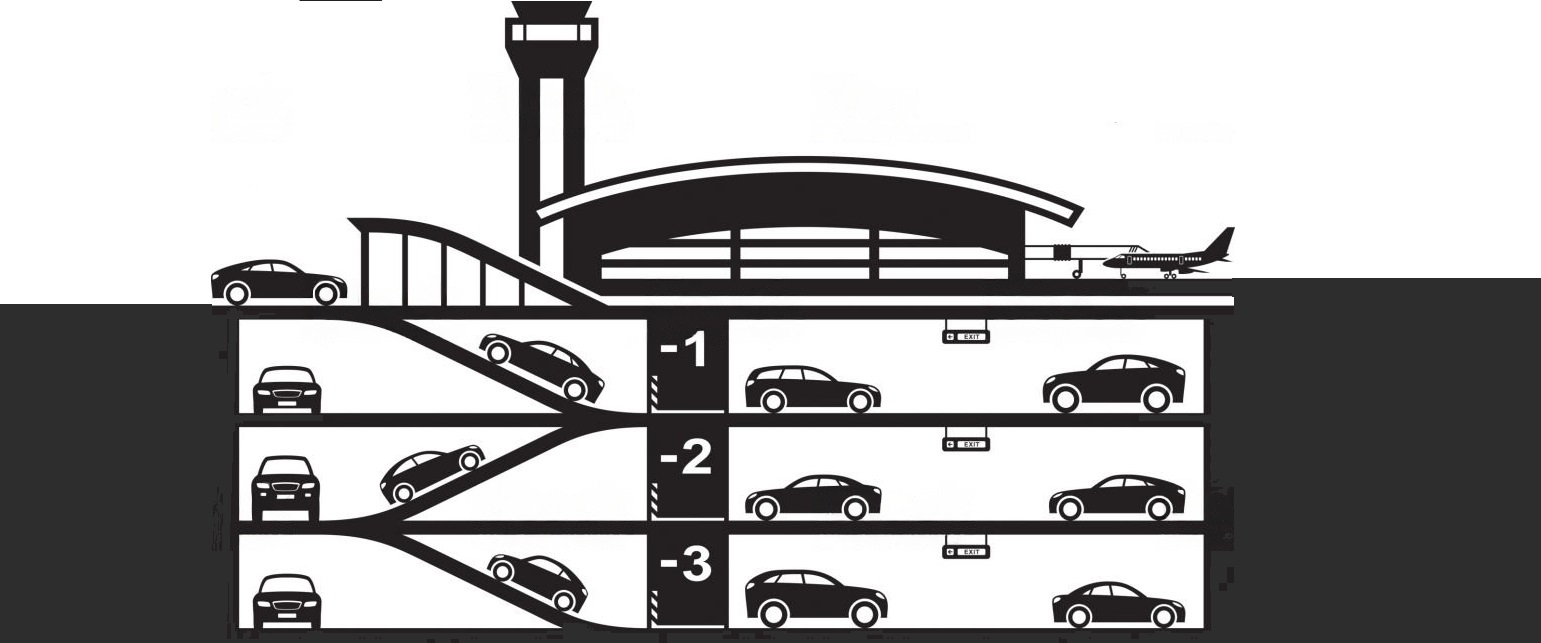
\includegraphics[height=06cm]{img/ch1-Underground parking garages-01.jpeg}
	\caption{Parc de stationnement souterrain}
 \label{Undergroundpark}
\end{figure}


\end{outline}

\subsection{Selon le mode de gestion}
Les types de parkings se différencient selon les modes de gestion en deux grands types, selon le paiement et la tarification, et selon l'accessibilité .

\subsubsection{Selon le mode de paiement}
Les parkings peuvent être classés en deux catégories principales, à savoir les parkings payants et les parkings gratuits.
\begin{outline}
    \1 \textbf{Stationnement payant par durée de stationnement/ illimité :} dans un parking payant, les utilisateurs doivent payer un montant prédéfinit ou un tarif forfaitaire  (quelle que soit la durée de stationnement) pour pouvoir se garer.
    \1 \textbf{Stationnement gratuit pour un temps limité/ illimité:}
    dans certains parkings gratuits, les utilisateurs peuvent stationner leur véhicule sans avoir à payer de frais pendant une durée limitée, généralement une ou deux heures. D'autres parkings gratuits offrent la possibilité de garer la voiture sans limite de temps. Ces parkings sont souvent situés dans des zones résidentielles ou des zones à faible trafic.
\end{outline}

Le choix entre un parking payant ou gratuit dépend souvent de la disponibilité, de la commodité, du coût et des préférences individuelles.

\subsubsection{Selon l'accessibilité}
On peut distinguer trois types de parkings en fonction de leur accessibilité : les parkings privés, les parkings publics et les parking privés à usage public \cite{lepermislibre}.

\begin{outline}
    \1  \textbf{Un parking public: } est un parking possédé et géré par des organismes publics, généralement la municipalité. Il est souvent situé en ville et hors agglomérations pour accueillir tous les usagers. Les parkings publics sont ouverts à tous, offrant ainsi une option de stationnement accessible à les usagers de la route.
    \1  \textbf{Un parking privé: } est un parking qui appartient et géré par des propriétaires privées ou des entreprises. Son accès peut être gratuit ou payant, et il peut être restreint par un badge ou une carte de stationnement. Les parkings privés sont généralement réservés aux clients, aux résidents ou aux employés d'un bâtiment spécifique, tel qu'un hôtel, un immeuble de bureaux ou un centre commercial. 
    \1  \textbf{Un parking privé à usage public: } est un parking appartenant à une entité privée qui est ouvert au public. 
    Un exemple courant de ce type de parking est celui des supermarchés. Ces parkings appartiennent au supermarché, mais ils sont accessibles à tous les clients qui souhaitent y circuler et s'y garer.

\end{outline}

Le choix entre un parking public et un parking privé dépend des circonstances individuelles, telles que l'emplacement, l'accès et les besoins spécifiques des conducteurs. 

\subsection{Selon la méthode de stationnement}
\begin{outline}
    \1  \textbf{Stationnement conventionnel: } est la méthode traditionnelle de stationnement où les conducteurs trouvent et occupent manuellement une place de stationnement. Les conducteurs conduisent leur véhicule jusqu'à le parc de stationnement disponible et effectuent les manœuvres nécessaires pour s'y garer. Cette méthode de stationnement est largement répandue et utilisée dans les parkings conventionnels.
    \1  \textbf{Stationnement robotisé (autonome): } il s'agit d'une méthode innovante où elle fait recours aux structures de stationnement automatisée (i.e systèmes robotiques) pour stationner et récupérer les véhicules sans intervention humaine. Dans ce type de système, les véhicules sont conduits jusqu'à une zone d'entrée spécifique où des capteurs et des logiciels avancés prennent le relais. Les véhicules sont guidés via les panneaux et signaux automatiques, puis déplacés automatiquement vers les emplacements de stationnement disponibles et les plus adaptés à leur taille à l'aide de mécanismes robotiques. Lorsque les conducteurs souhaitent récupérer leur véhicule, celui-ci est ramené à la zone de sortie par le système automatisé. Ce type de stationnement offre de nombreux avantages notamment l'utilisation optimisée de l'espace, une meilleure efficacité du stationnement et une réduction des risques de collision. l'illustration dans la figure  \ref{Automaticcarpark} 
    
\begin{figure}[H]
	\centering
	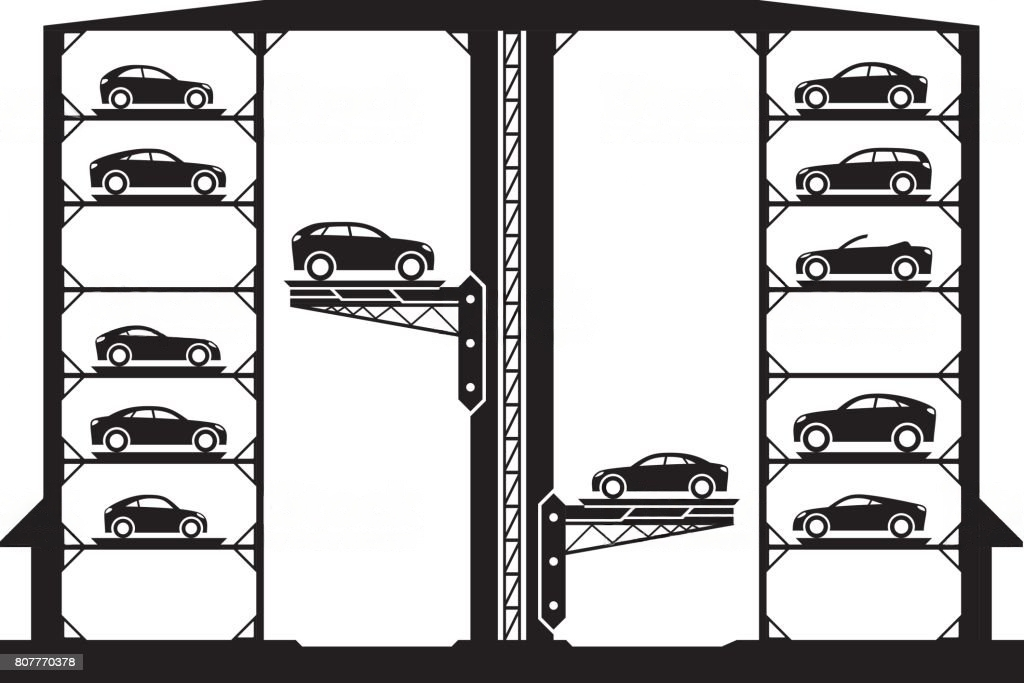
\includegraphics[height=06cm]{img/ch1-Automatic car parking -01.jpeg}
	\caption{Parc avec stationnement autonome}
 \label{Automaticcarpark}
\end{figure}



\end{outline}

\section{Gestion des parkings}

La gestion des parkings peut varier en fonction du niveau d'automatisation impliqué \cite{bensalah-master}. On peut distinguer trois types principaux de gestion de parking :

\begin{outline}

\1  \textbf{Une gestion manuelle: } dans un parking à gestion manuelle, 
toutes les opérations sont effectuées par le personnel de service. Cela inclut l'accueil des conducteurs, la collecte des frais de stationnement, l'orientation vers les places disponibles et la surveillance générale du parking. 
Les employés sont responsables de toutes les tâches liées à la gestion du parking, au guidage des conducteurs et l'enregistrement de toutes les informations relatives aux parkings, que ce soit dans un registre ou dans un système informatique. Lors de leur arrivée au parking, les automobilistes reçoivent un ticket (en papier ou de bons d'entrée) et doivent le présenter au personnel de service lorsqu'ils quittent le parking pour régler les frais de stationnement. Ce type de système est généralement utilisé dans les petits parkings ou dans les zones où l'automatisation n'est pas encore largement répandue. Toutefois, il  présente une consommation importante de ressources et est sujet à de nombreuses erreurs et corruptions.


\1  \textbf{Une gestion semi-automatique: } dans un parking à gestion semi-automatique, certains aspects du processus de gestion sont automatisés pour améliorer l'efficacité. Par exemple, l'accueil des conducteurs et la collecte des frais de stationnement peuvent être effectués à l'aide de systèmes de paiement automatisés ou de bornes de paiement. De plus, des panneaux électroniques peuvent être utilisés pour indiquer les places disponibles. Ainsi que des barrières d'entrée et de sortie automatisées peuvent être utilisée pour contrôler l'accès des véhicules. Cependant, certaines tâches nécessitent toujours une intervention humaine, comme l'orientation des conducteurs vers les places de stationnement qui se fait par un agent de stationnement. Ce type de système offre une certaine automatisation tout en conservant une certaine interaction humaine.


\1 \textbf{Une gestion entièrement automatisée: } Dans un parking à  gestion automatisée, la majorité, voire toutes les opérations de gestion sont automatisées et aucune intervention humaine n'est nécessaire. 
Des systèmes informatisés ainsi que des technologies avancées sont utilisés pour effectuer toutes les opérations de gestion du stationnement notamment la collecte des frais de stationnement, l'orientation des conducteurs vers les places disponibles et la surveillance du parking. Ces systèmes offrent une gestion plus efficace et souvent utilisés dans les parkings à grande échelle ou dans les zones à forte densité de circulation.

\end{outline}
La méthode de gestion du stationnement à adopter dépend des besoins spécifiques de chaque emplacement et des ressources disponibles pour sa mise en œuvre.

\section{Systèmes de gestion des parkings}

Les systèmes de gestion des parkings sont des solutions technologiques utilisées pour optimiser l'efficacité et la gestion des parkings. Ils peuvent inclure une variété de fonctionnalités et d'outils pour faciliter la réservation, le contrôle d'accès, la collecte des frais de stationnement, la surveillance en temps réel, la gestion des données et la génération de rapports sur l’occupation du parking et la génération de revenus. 

Les parkings dotés de systèmes de gestion intègrent généralement les fonctionnalités suivantes:

\begin{enumerate}
   \item [$\bullet$]  Guidage des véhicules: Les parcs de stationnement automatisés sont équipés de systèmes de guidage qui aident les conducteurs à trouver rapidement des places de stationnement disponibles. Cela peut inclure des panneaux indicateurs, des feux de signalisation et des indications visuelles pour diriger les conducteurs vers les emplacements libres.
    \item [$\bullet$]  Contrôle d'accès automatisé : Les parcs de stationnement automatisés utilisent des systèmes de contrôle d'accès automatisés pour gérer l'entrée et la sortie des véhicules. Cela peut se faire à l'aide de cartes magnétiques, de codes QR, de lecteurs de plaques d'immatriculation ou d'autres technologies d'identification et de reconnaissance.
     \item [$\bullet$] Comptage de véhicules : Pour connaître l'état du parking, des capteurs en temps-réel sont utilisés pour compter le nombre de véhicules présents dans le parking, le nombre de places occupées/vacantes, fournissant des données précieuses pour la gestion et la planification.
   \item [$\bullet$] Empilement automatique des véhicules : Dans des parcs à espace limité, les véhicules sont empilés et stockés de manière automatisée grâce à des systèmes mécanisés d'empilement. Cela permet d'optimiser l'utilisation de l'espace en réduisant l'encombrement et en permettant le stationnement de plus de véhicules dans une superficie limitée.
    \item [$\bullet$] Surveillance temps-réel et sécurité renforcée : Les parcs de stationnement automatisés sont équipés de mesures de sécurité avancées, telles que des caméras de surveillance, des systèmes d'alarme et des dispositifs de sécurité pour assurer la protection des véhicules et des utilisateurs.
    \item [$\bullet$] Paiement automatisé : Pour permettre 
   aux utilisateurs de régler facilement les frais de stationnement, les parcs peuvent être équipés des bornes de paiement automatisée.
   Ces bornes peuvent accepter différents modes de paiement, tels que 
   le paiement sans contact ou paiement mobile.
   \item [$\bullet$] Gestion des abonnements : Permettant aux abonnés d'accéder facilement au parking en utilisant des cartes bancaires, ou des badges d'abonnement, en offrant donc  un accès rapide et pratique aux abonnées.
  \item [$\bullet$] Gestion de réservation: Permettant aux utilisateurs de réserver à l'avance une place de stationnement dans le parking, garantissant ainsi leur disponibilité lors de leur arrivée. Elle est effectuée en ligne, généralement via un site Web ou une application mobile dédiée.
   \item [$\bullet$] Génération de rapports d'activité : Est une fonctionnalité essentielle. Les rapports d'activité fournissent des informations détaillées sur divers aspects du fonctionnement du parking telles que le nombre de véhicules entrants et sortants, la durée de stationnement moyenne, l'occupation du parking en temps réel, les revenus générés, les tendances de fréquentation, les heures de pointe, etc. Les données collectées par les différents outils du système, tels que les capteurs de stationnement, les dispositifs de paiement et les caméras de surveillance, sont centralisées et analysées pour produire des rapports pertinents. Les rapports peuvent être consultés à tout moment par les gestionnaires du parking, ce qui leur permet de suivre les performances du parking, de prendre des décisions éclairées basées sur des données concrètes et d'optimiser les opérations.

\end{enumerate}

En plus de ces fonctionnalités, d'autres technologies peuvent être intégrés, telles que les applications mobiles qui offrent aux utilisateurs des fonctionnalités pratiques telles que la recherche de places, la réservation, le paiement et la navigation vers le parking.

Le contrôle de l'ensemble du processus de stationnement se fait d'une manière centralisé via un système informatisé ou un logiciel de gestion du stationnement qui regroupe toutes les fonctionnalités nécessaires et assure une coordination efficace de l'ensemble du processus de stationnement. 
La sélection et la mise en place d'un système de gestion des parkings dépendent des besoins spécifiques de chaque site, de sa taille, de son type d'utilisation et des ressources disponibles. 

L'objectif de tels systèmes est d'améliorer l'expérience des utilisateurs (i.e expérience plus pratique), d'optimiser l'utilisation de l'espace de stationnement et des ressources disponibles, de réduire la congestion, d'augmenter la sécurité et d'optimiser la gestion des revenus.

Il est donc courant d'utiliser une combinaison d'outils pour créer un système de gestion du stationnement complet et efficace. 


\section{Outils utilisés dans un système de gestion du stationnement}
Dans un parking, les outils et les personnes ont des fonctions différentes mais complémentaires.

Dans le cadre d'un système de gestion automatique du stationnement, différents outils sont utilisés pour optimiser la gestion des parkings et des véhicules. Bien que le rôle du personnel travaillant dans le parking soit généralement réduit par rapport à un système traditionnel, leur présence demeure importante pour offrir une assistance en cas de problèmes ou des situations imprévues. Leur présence garantit une expérience client optimale et contribue à assurer le bon fonctionnement global du système de gestion automatique du stationnement.

Parmi les outils basiques utilisés, on retrouve les barrières et les portes tournantes qui sont utilisées pour contrôler l'accès des véhicules au parking, ainsi que les portillons sont employés pour restreindre l'accès des piétons à certaines zones. Les caméras de surveillance et les systèmes d'interphone aident également à améliorer la sécurité et la surveillance, permettant aux opérateurs de surveiller les activités dans le parking. De plus, les panneaux de signalisation sont installés pour informer les conducteurs et les piétons des règles et des réglementations du parking. Tous ces équipements sont généralement gérés par un système informatisé.

En parallèle, le personnel travaillant dans le parking peut effectuer des tâches telles que la surveillance générale du système, l'assistance aux utilisateurs en cas de besoin, la résolution de problèmes techniques et le maintien de la propreté et de l'ordre dans le parking. Ils peuvent également être disponibles pour fournir des informations et des orientations aux conducteurs ou pour gérer des situations d'urgence. Leur rôle se concentre davantage sur la surveillance, l'assistance et la résolution de problèmes plutôt que sur des tâches manuelles directes liées à la gestion du stationnement.

\subsubsection{ Les barrières d'entrée et de sortie}
Les barrières dans les parkings sont des dispositifs physiques qui sont installés à l'entrée et à la sortie d'un parking pour contrôler l'accès des véhicules et réguler le flux de circulation. Les barrières sont généralement associées à des systèmes de paiement pour le stationnement et peuvent être manuelles ou automatiques. un exemple de barrière est montré dans l'image \ref{ch1barrier}.

\begin{figure}[H]
	\centering
	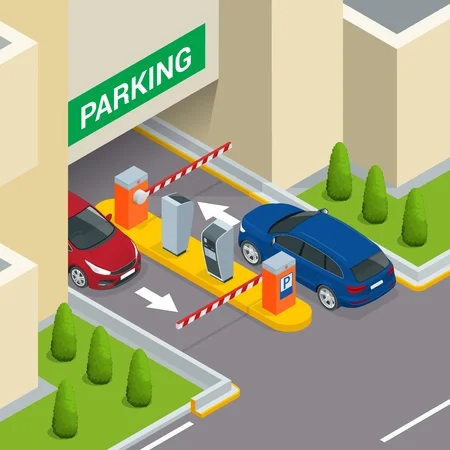
\includegraphics[height=06.2cm]{img/ch1-barrier-01.jpg}
	\caption{ Barrières d'entrée et de sortie}
  \label{ch1barrier}
\end{figure}

\textbf{1- Les barrières manuelles : } sont actionnées manuellement par un opérateur, qui contrôle l'accès des véhicules à l'entrée et à la sortie du parking en levant ou abaissant la barrière à l'aide d'une télécommande ou d'un levier. Les barrières manuelles sont souvent utilisées dans les petits parkings ou les parkings résidentiels où il y a un trafic relativement faible et où il n'est pas nécessaire de contrôler l'accès de manière automatique.

\textbf{2- Les barrières automatiques : } sont actionnées par un système électronique et sont équipées de capteurs de mouvement qui détectent la présence d'un véhicule. Lorsqu'un véhicule s'approche de la barrière, le système électronique déclenche l'ouverture ou la fermeture de la barrière pour permettre ou interdire l'accès. Les barrières automatiques sont souvent utilisées dans les parkings publics ou commerciaux où il y a un trafic plus important et où il est nécessaire de contrôler l'accès de manière efficace.

\subsubsection{ Les panneaux de signalisation}
Les panneaux de signalisation dans les parkings aident les conducteurs et les piétons à naviguer dans le parking en leur fournissant des informations sur la circulation, le stationnement et les règles de sécurité. Ils permettent est de faciliter la circulation et le stationnement des véhicules, de minimiser les risques d'accidents et de garantir la sécurité des piétons. Les panneaux doivent être clairs, visibles et conformes aux normes de signalisation routière en vigueur. Ils peuvent être fixes ou électroniques et être accompagnés d'autres dispositifs de contrôle de la circulation.
voici quelques panneaux dans l'image suivante \ref{ch1plak}

\begin{figure}[H]
	\centering
	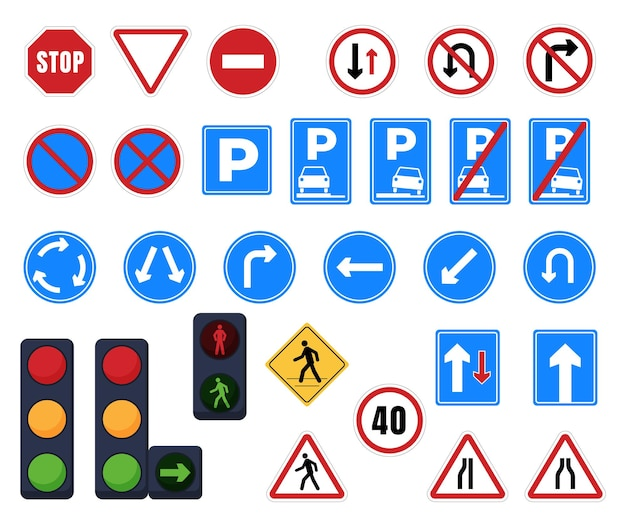
\includegraphics[height=06.5cm]{img/ch1-plak-01.jpg}
	\caption{Panneaux de signalisation}
 \label{ch1plak}
\end{figure}


\subsubsection{Les capteurs de stationnement}
Les capteurs utilisés dans les parkings sont des dispositifs électroniques qui sont conçus pour détecter la présence de véhicules dans une place de stationnement. Ces capteurs peuvent être installés dans les surfaces de stationnement, tels que les planchers ou les trottoirs, et peuvent être connectés à un système de gestion de parking pour surveiller l'occupation des places de stationnement en temps réel.

Les capteurs peuvent fonctionner de différentes manières, mais la plupart utilisent des technologies telles que les ultrasons, les champs magnétiques ou les capteurs de pression pour détecter la présence d'un véhicule. Certains capteurs peuvent également mesurer la durée de stationnement des véhicules et signaler tout dépassement de temps. l'image au dessous \ref{ch1sensor} illustre un des types de capteurs de rue 

\begin{figure}[H]
	\centering
	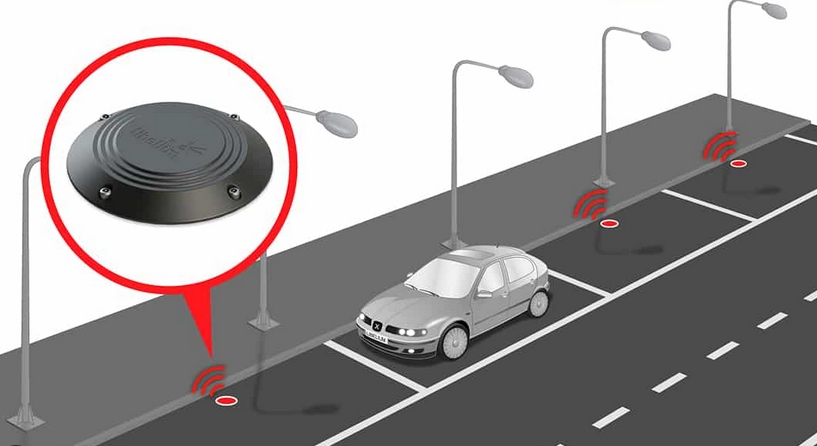
\includegraphics[height=05cm]{img/ch1-sensor-01.jpg}
	\caption{Les capteurs}
 \label{ch1sensor}
\end{figure}

% \subsubsection{ Les lecteurs de plaques d'immatriculation}

% Les lecteurs de plaques d'immatriculation, également appelés systèmes de reconnaissance automatique des plaques d'immatriculation comme montre la figure \ref{img}, sont des dispositifs utilisés dans les parkings pour capturer et reconnaître les plaques d'immatriculation des véhicules entrant et sortant. Ces lecteurs utilisent des caméras spéciales et des logiciels de reconnaissance optique des caractères pour analyser les images des plaques d'immatriculation et extraire les informations textuelles.

% L'objectif principal de ces systèmes est d'automatiser le processus d'identification des véhicules ce qui facilite par conséquent la traçabilité des véhicules dans le parking. Grâce à  cette automatisation, les erreurs humaines liées à la saisie manuelle des informations sont réduites.
% Les informations extraites des plaques d'immatriculation sont enregistrées dans le système de gestion du parking qui peut également enregistrer les données relatives aux véhicules entrants et sortants, telles que l'heure d'entrée et de sortie, la durée de stationnement, les transactions de paiement, etc. Ces données sont traités de manière sécurisée et conforme aux réglementations sur la protection des données personnelles. Des mesures appropriées doivent être prises pour garantir la sécurité et la confidentialité des données.

% \begin{figure}[H]
% 	\centering
% 	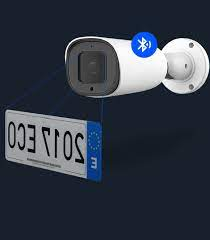
\includegraphics[height=05cm]{ch2-plate_read.jpg}
% 	\caption{Lecteurs de plaques d'immatriculation}
%  \label{img}
% \end{figure}

\subsubsection{Les bornes de paiement}
Les bornes de paiement \ref{img1} utilisées dans les parking sont des dispositifs électroniques autonomes qui offrent aux utilisateurs différentes options pour effectuer des paiements de manière automatisée (rapide, pratique et sécurisée) sans avoir besoin d'interagir avec un caissier ou un employé. En plus du paiement, ces bornes ont également la capacité d'émettre des tickets de paiement \cite{ch2_Transpor19}.

Lorsqu'un utilisateur souhaite payer son stationnement, il peut utiliser des cartes de bancaires, insérer des pièces de monnaie, des billets de banque ou utiliser des badges d'abonnement. Certaines bornes de paiement prennent également en charge les paiements mobiles, permettant aux utilisateurs de payer via des applications mobiles ou des portefeuilles électroniques. Ces options de paiement offrent aux utilisateurs une flexibilité lorsqu'ils règlent leurs frais de stationnement.
Une fois le paiement effectué, la borne génère un ticket de paiement qui sert de preuve de paiement et de validation du stationnement.

\begin{figure}[H]
	\centering
	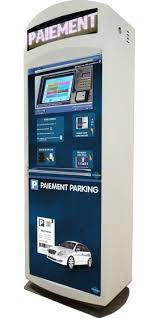
\includegraphics[height=07cm]{ch2-Bornes_pay.jpg}
	\caption{ Bornes de paiement}
 \label{img1}
\end{figure}

\section{Étude d'existant}

L'étude de l'existant en matière de systèmes de gestion de parking en Algérie révèle une diversité de solutions utilisées dans différents parkings à travers le pays. La plupart des parkings publics qu'on a visité utilisent des systèmes de gestion traditionnels basés sur des tickets papier ou des barrières manuelles gérées par le personnel.
On cite dans ce qui suit cinq exemples de parkings où ces méthodes sont en place :
\subsection{Parking Bézier - Tafourah - Alger}



Il s'agit d'un parking à plusieurs étages, public pour tous, et l'argent payé est calculé en fonction de la durée de stationnement

Lorsque vous arrivez à l'entrée du parking, vous trouverez un employé qui notera la plaque d'immatriculation du véhicule et l'heure d'entrée et vous remettra un ticket

Le ticket contient un table composé des heures de la journée de 6 h à 23 h

L'heure que vous avez entrée est cochée afin que vous sachiez à quelle heure vous avez entré

Vous recherchez un endroit pour garer la voiture et la garer

Et quand vous voulez quitter le parking, vous donnez ce ticket à un employé, et il calcule le temps approximatif que cela a pris et vous indique le prix.

Le prix le plus bas qui peut être payé est de 100 dinars si cela prend moins ou égal à 2 heures, et après les deux premières heures, 50 dinars seront ajoutés par heure. 
au dessous \ref{Bézier} une image réelle du parking Bézier qui se situe à Tafourah - wilaya d'Alger.

\begin{figure}
	\centering
	\includegraphics[height=07.5cm]{img/ch2-Parking Bézier - Tafourah - Alger.jpg}
	\caption{Parking Bézier - Tafourah - Alger}
 \label{Bézier}
\end{figure}

\subsection{Parking de l'université d'Alger1 - Ben Youssef Ben Khadda - Alger}  



C'est un parking pour les employés travaillant à l'université \ref{Khadda}, l'entrée est la même que la sortie, et il est géré par des personnes sans aucun outil technologique.

Lorsque le véhicule arrive à l'entrée du parking, le gardien vérifie son droit d'entrée en reconnaissant le conducteur du véhicule, ou le conducteur du véhicule voyant la carte de droit d'accès.

Si le gardien décide d'entrer dans le véhicule, il ouvre la porte, laisse entrer le véhicule et commence à chercher une place pour garer le véhicule.

L'un des plus gros problèmes dont souffre cette situation est que le propriétaire de la voiture ne sait pas s'il y a une place disponible pour garer sa voiture, et il peut devoir chercher et perdre du temps, puis quitter le parking pour chercher une place. Garez la voiture ailleurs.

\begin{figure}[H]
	\centering
	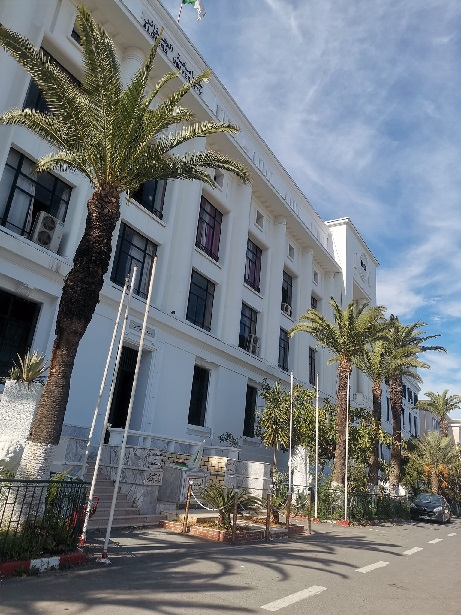
\includegraphics[height=07.5cm]{ch2-Parking de l'université centrale, Université Yusuf bin Khadda.jpg}
	\caption{Parking de l'université d'Alger1 - Ben Youssef Ben Khadda - Alger}
 \label{Khadda}
\end{figure}

% \subsection{ Parking avec ascenseur - centre d'Oran}
% Ce parking à plusieurs étages est équipé d'un ascenseur pour faciliter l'accès aux différents niveaux.
% À l'entrée du parking, un membre du personnel du parking remet un ticket manuscrit au propriétaire de la voiture. Ce dernier est alors invité à laisser les clés de sa voiture et à indiquer l'heure de retour prévue pour la récupérer.

\subsection{Parking Ali Mellah - premier mai - Alger}
C'est un parking semi-automatique où, quand le chauffeur arrive à l'entrée du parking, un agent vous extrait  un ticket apartir d'une machine, puis le client rentre et cherche un espace vide pour garer son voiture.
À la sortie le chauffeur donne le ticket à un autre agent afin de calculer le montant à payer.

\subsection{Parking de l'aéroport Houari Boumédiène - Alger}
Le parking en question est un parking en surface accessible au public \ref{Boumédiène}, et les frais de stationnement sont calculés en fonction de la durée de stationnement.
\\
Lorsqu'un véhicule arrive au parking, il se trouve face à une barrière fermée munie d'un bouton. En appuyant sur ce bouton, un ticket est généré, comprenant un QR-code ainsi que d'autres informations pertinentes. Par la suite, la barrière s'ouvre, permettant ainsi au véhicule d'accéder au parking.
\\
En ce qui concerne le paiement, une borne de paiement est mise à disposition pour effectuer le règlement en espèces, que ce soit sous forme de billets ou de pièces. De plus, la borne est en mesure de rendre la monnaie si nécessaire.
\\
Une fois le paiement effectué, il est important de sortir rapidement du parking en se dirigeant vers la sortie désignée. À la sortie, une barrière est présente et s'ouvre en scannant le QR-code présent sur le ticket.
\\
Dans le cas où le paiement n'a pas été effectué, il est nécessaire de se rendre à une sortie spécifique où un poste de garde est situé. A cette endroit, il sera possible de régler les frais de stationnement pour pouvoir quitter le parking.
\begin{figure}[H]
	\centering
	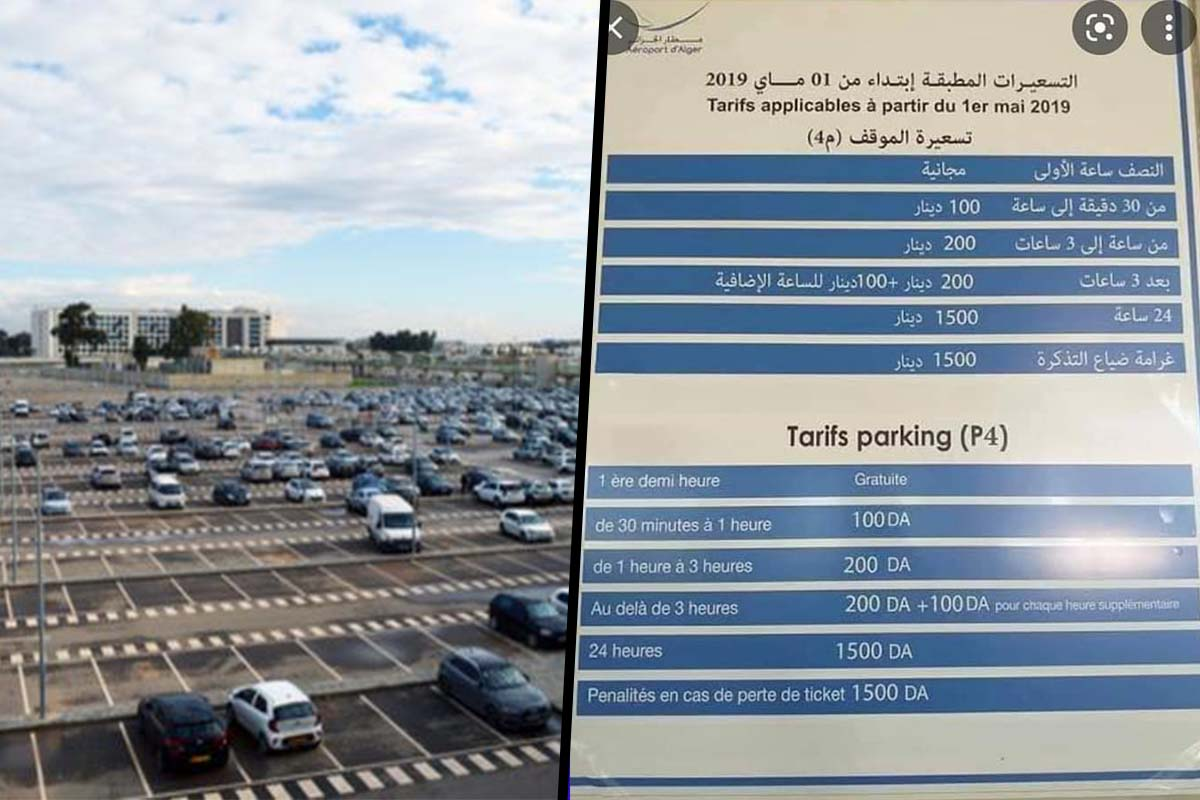
\includegraphics[height=08cm]{img/ch2-Parking aéroport à Alger Houari Boumédiène Airport.jpg}
	\caption{Parking de l'aéroport Houari Boumédiène}
 \label{Boumédiène}
\end{figure}
L'aéroport adopte une technologie de paiement électronique pour les cartes de stationnement, selon laquelle le propriétaire de la voiture doit payer la valeur du billet en fonction des heures d'attente dans un dispositif électronique qui lui donne une carte de dégagement de manière automatique, lui permettant de sortir automatiquement de la porte.

  
\textbf{L'étude réalisée met en évidence les lacunes suivantes dans les systèmes de gestion de parking :}
\begin{enumerate}
   \item [$\bullet$] Congestion à l'entrée et à la sortie du parking : Les barrières manuelles ou les méthodes de paiement traditionnelles peuvent entraîner des files d'attente importantes, ce qui provoque des embouteillages aux heures de pointe.
   \item [$\bullet$] Difficulté à trouver une place de stationnement : En raison de l'absence de visibilité sur les places disponibles, les conducteurs peuvent perdre du temps à chercher une place pour garer leur voiture, ce qui entraîne des retards et de la frustration.
   \item [$\bullet$] Manque d'information sur la disponibilité des places : Les conducteurs n'ont pas d'indications en temps réel sur la disponibilité des places de stationnement, ce qui les oblige à entrer dans le parking sans savoir s'il y a des espaces vacants.
   \item [$\bullet$] Stationnement désorganisé : En l'absence d'un système de guidage efficace, les voitures sont souvent garées de manière aléatoire à l'intérieur du parking, ce qui rend difficile la recherche d'une place disponible.
   \item [$\bullet$] Risque de perte du billet de stationnement : Si un conducteur perd son billet de stationnement, il peut être confronté à des frais supplémentaires ou à des difficultés pour sortir du parking.
   \item [$\bullet$] Manque de sécurité : Les systèmes de gestion actuels nécessitent souvent de laisser les clés de la voiture au personnel du parking, ce qui peut créer des risques de vol ou d'utilisation non autorisée du véhicule.
\end{enumerate}
Ces lacunes soulignent la nécessité d'améliorer les systèmes de gestion de parking en utilisant des technologies avancées. Ces solutions permettraient d'optimiser l'utilisation de l'espace de stationnement, de réduire les embouteillages, d'améliorer la sécurité et de faciliter l'expérience des conducteurs.

\section{Conclusion}

Dans le premier chapitre, nous avons abordé les divers aspects des parkings, notamment les différents types de parkings, la gestion des parkings et les systèmes de gestion des parkings. Nous avons présenté également les outils utilisés dans un système de gestion des parkings et procédé à une étude de l'existant pour mieux cerner les problèmes auxquels sont confrontés les parkings étudiés.
Dans le chapitre deux, nous nous penchons sur l'apprentissage automatique et la vision par ordinateur.
%---------------------------------------------------------------
%-- https://en.wikipedia.org/wiki/Parking
%-- https://codedelaroute.io/blog/parking-public/
%-- https://www.yespark.fr/edito/lexique-parking/parking-public-prive-definition-reglementation
%-- https://les-fourrieres.fr/guides-actualites/parking-prive-a-usage-public-quelles-sont-les-regles/
%-- https://parking-gery.com/9095_Quelle-est-la-difference-entre-un-parking-public-et-un-parking-prive-.html
%-- 
%-- 
%-- 
%-- 


\chapter{Apprentissage profond et détection d'objet: Concepts et algorithmes}
\markboth{Apprentissage profond et détection d'objet: Concepts et algorithmes}{}
\section{Introduction}
%%%%%%%%%\Ajouter l'architecture YOLOV8%%%%%%%%%%%%%%%%
Au cours des vingt dernières années, des technologies avancées telles que l'intelligence artificielle, l'apprentissage automatique et la vision par ordinateur sont passées de la recherche et du développement à des environnements commerciaux et grand public.
\\
L'adaptation commerciale a vu des chaînes de montage automatisées de production de robots, des systèmes de guidage automatisés de véhicules et l'analyse d'images capturées à distance pour faciliter les stratégies d'inspection visuelle automatisées. En conséquence, les applications de vision par ordinateur et d'apprentissage automatique font partie des sujets techniques les plus séduisants et les plus fascinants de nos jours. Et la plupart des entreprises modernes de l'industrie technologique et des start-ups technologiques ambitieuses se précipitent pour profiter des avantages de ces technologies de pointe.
\\
Les progrès de l'apprentissage automatique et de la vision par ordinateur ont eu un impact significatif sur divers secteurs industriels, y compris la gestion des parkings. Grâce à ces technologies avancées, les machines sont capables d'apprendre à partir de données et de traiter diverses informations, offrant ainsi de nouvelles possibilités pour optimiser les performances de la gestion des parkings.
\\
Dans ce chapitre, nous explorons en détail l'apprentissage profond et ses différentes architectures. Nous fournissons également un aperçu des principaux algorithmes développés spécifiquement pour la détection d'objets. Enfin, nous présentons différentes mesures de performance essentielles pour évaluer les modèles de classification et les détecteurs d'objet.

\section{Intelligence artificielle }
L'intelligence artificielle (IA) fait référence à la théorie et au développement de systèmes informatiques capables d'effectuer des tâches qui nécessitent généralement l'intelligence humaine, telles que la perception visuelle, la reconnaissance de la parole, la prise de décision et la traduction entre les langues et bien d'autres. Le terme est fréquemment utilisé pour décrire des systèmes conçus pour imiter les processus intellectuels humains, tels que la capacité de raisonner d'apprendre, de percevoir, de comprendre et d'interagir avec l'environnement de manière autonome \cite{Questceq75}.
\\
C'est un domaine domaine interdisciplinaire  qui regroupe plusieurs sous-domaines, notamment l'apprentissage automatique et la vision par ordinateur.

\section{Apprentissage automatique}
L'apprentissage automatique (machine learning; ML) est l'un des outils principaux utilisés dans les systèmes d'intelligence artificielle pour résoudre des problèmes complexes et effectuer des tâches intelligentes telles que la reconnaissance d'images, le traitement du langage naturel, la recommandation de produits, la détection de fraudes, etc.
\\
Le principe de base de l'apprentissage automatique repose sur la capacité d'un ordinateur à apprendre à partir de données sans être explicitement programmé
pour détecter des schémas, des tendances et des relations cachées. Il utilise ces informations pour générer des modèles et effectuer des prédictions sur de nouvelles données.
\\
Dans l'apprentissage automatique, on distingue quatre types d'approches: l'apprentissage supervisé, l'apprentissage non supervisé, l'apprentissage semi-supervisé et l'apprentissage par renforcement. Ces approches, comme illustré dans la figure \ref{fig:ch2-ml-tree-01}, peuvent être indépendamment utilisées ou combinées avec l'apprentissage profond pour résoudre divers problèmes \cite{ch_Deep_Learning}.

Dans la section suivante, nous allons expliquer brièvement chacune de ces approches.

L'apprentissage superficiel utilise des algorithmes de l’apprentissage automatique simples pour apprendre à partir de données, tandis que l'apprentissage en profondeur utilise des réseaux de neurones artificiels à plusieurs couches pour apprendre des représentations de données hiérarchiques et abstraites. 

L'apprentissage en profondeur est capable de capturer des modèles plus complexes dans les données que l'apprentissage peu profond, mais il peut nécessiter plus de données annotées pour obtenir des résultats précis.

\subsection{Paradigmes d'apprentissage automatique}
Comme illustré dans la figure \ref{fig:ch2-ml-tree-01}, le domaine de l’apprentissage automatique est souvent divisé en approches supervisées, non supervisées, semi-supervisées et par renforcement, en fonction du type de problème à résoudre.

\begin{figure}[H]
	\centering
	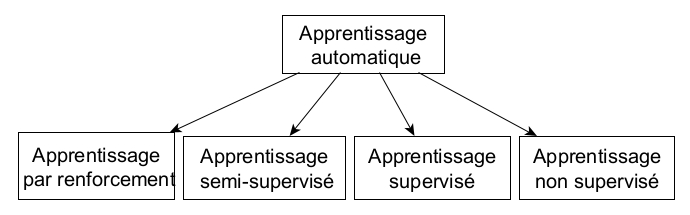
\includegraphics[height=5cm]{ch2-ml-tree-01.jpg}
	\caption{Paradigmes d'apprentissage automatique}
    \label{fig:ch2-ml-tree-01}
\end{figure}

\begin{enumerate}
\item [$\bullet$] \textbf{Apprentissage supervisé} : dans ce type d'apprentissage, les algorithmes sont entraînés sur des données étiquetées. 
Une fois que le modèle est généré, il peut être utilisé pour faire des prédictions sur de nouvelles données en inférant les étiquettes correspondantes en fonction des caractéristiques observées.\\
Les problèmes d'apprentissage supervisé peuvent être catégorisés en deux types principaux : la régression et la classification. Dans la régression, l'objectif est de prédire une valeur numérique continue. Les algorithmes couramment utilisés pour la régression comprennent la régression linéaire, la régression à vecteurs de support, les arbres de régression, les forêts aléatoires, et les réseaux de neurones de régression.
\\
Dans la classification, l'objectif est de prédire une étiquette ou une classe spécifique. Les algorithmes couramment utilisés pour la classification comprennent les arbres de décision, les forêts aléatoires, les machines à vecteurs de support (SVM), les méthodes de régression logistique, les réseaux de neurones et les algorithmes de classification bayésienne \cite{ch_Deep_Learning}.

\item [$\bullet$] \textbf{Apprentissage non supervisé} : cherche à identifier des structures, des modèles (patterns) ou des relations dans les données non étiquetées. Cela peut être réalisé à l'aide de techniques telles que le partitionnement de données (clustering), la réduction de dimensionalité, les règles d'association \cite{ch_Deep_Learning}, etc. 

\item [$\bullet$] \textbf{Apprentissage semi-supervisé } : est une combinaison des deux types d'apprentissage précédents, où le modèle est généré en utilisant à la fois des données étiquetées et non étiquetées. Cette méthode est utile lorsque les données étiquetées sont limitées ou coûteuses à obtenir. Elle vise à exploiter les informations contenues dans les données non étiquetées pour améliorer les performances de généralisation du modèle.
\\
Les algorithmes d'apprentissage semi-supervisé impliquent généralement deux étapes principales : l'entraînement initial sur les données étiquetées et la propagation des étiquettes aux données non étiquetées. L'entraînement initial est effectué à l'aide des exemples étiquetés pour construire un modèle de prédiction. Ensuite, les étiquettes prédites sont exploitées pour prédire les étiquettes des exemples non étiquetés \cite{semi-supervise_chapelle2006semi}.

\item [$\bullet$] \textbf{Apprentissage par renforcement} : est une technique d'apprentissage automatique où un agent apprend à prendre des décisions dans un environnement en interagissant avec celui-ci. L'agent reçoit des récompenses ou des pénalités en fonction de ses actions et apprend à optimiser ses actions pour maximiser les récompenses à long terme. Parmi les algorithmes les plus reconnus de l'apprentissage par renforcement, on peut citer Q learning \cite{q_learning_01} et policy gradient \cite{policy_gradient_01}.
\end{enumerate}
Le choix du modèle d'apprentissage à appliquer dépend de la nature des données disponibles,de la complexité du problème, des ressources disponibles et des objectifs spécifiques de l'application.
\section{Apprentissage profond}
L'apprentissage profond (connu sous le nom de deep learning en anglais) a provoqué une véritable révolution dans le domaine de l'apprentissage automatique. Il a ouvert la voie à la création de modèles de plus en plus complexes et, dans une certaine mesure, plus précis, capables de résoudre des problèmes difficiles dans les domaines de la vision par ordinateur, le traitement du langage naturel, la reconnaissance vocale, et bien d'autres encore \cite{ch_Deep_Learning}.

Ces avancées ont surmonté les limitations des méthodes classiques d'apprentissage en termes de performances. En effet, ces méthodes nécessitent souvent une intervention humaine pour extraire des caractéristiques significatives à partir des données d'entrée, ce qui a limité leur capacité de  généralisation \cite{ch_Deep_Learning}.

Avant l'émergence de l'apprentissage en profondeur, les méthodes d'apprentissage automatique étaient principalement basées sur des algorithmes d'apprentissage supervisé ou non supervisé tels que les arbres de décision, les k-means, les SVM, etc. Ces méthodes étaient limitées par la complexité des modèles qu'elles pouvaient créer et leur capacité à gérer des données complexes et non structurées. Elles nécessitaient souvent une intervention humaine pour extraire des caractéristiques significatives à partir des données d'entrée, ce qui limitait leur capacité à généraliser à de nouvelles données \cite{ch_Deep_Learning}.

L'apprentissage profond repose sur l'utilisation des réseaux de neurones artificiels profonds (DNN), qui permettent une représentation hiérarchique à partir de données brutes sans avoir besoin d'une intervention humaine pour sélectionner des caractéristiques significatives. 
Les DNN sont composés de  multiple couches cachées empilées. Cette architecture en couches contribue à la flexibilité des modèles. Chaque couche apprend à reconnaître des caractéristiques de plus en plus abstraites et complexes. Cela permet au modèle de détecter des relations et de différents patterns dans les données(souvent complexes), ce qui conduit à des prédictions plus précises et à des performances améliorées \cite{ch_Deep_Learning}.

\subsection{Réseaux de neurones artificiels}
Les réseaux de neurones artificiels sont des modèles d'apprentissage statistiques qui imitent le fonctionnement du cerveau humain pour résoudre des problèmes complexes d'apprentissage automatique. Ils sont généralement utilisés pour résoudre des problèmes de classification, de régression et de prédiction \cite{ch_Deep_Learning}.

Un réseau de neurones artificiels est composé des couches de neurones interconnectés. Chaque neurone reçoit des signaux d'entrée pondérés, effectue des calculs sur ces signaux et transmet une sortie à d'autres neurones. Ces connexions entre les neurones sont associées à des poids qui déterminent l'importance de chaque connexion \cite{ch_Deep_Learning}.

L'apprentissage des réseaux de neurones est réalisé par l'ajustement des poids des connexions, de manière à minimiser une fonction d'erreur. Cela se fait généralement à l'aide d'une technique appelée rétropropagation du gradient, qui utilise la dérivée de la fonction d'erreur par rapport aux poids pour mettre à jour les poids du réseau \cite{ch_Deep_Learning}.

Il existe plusieurs types de réseaux de neurones profonds, chacun avec une architecture différente pour résoudre des problèmes spécifiques. Les types de réseaux de neurones artificiels courants incluent :

\begin{outline}
\1  Les réseaux de neurones multi-couches (MLP), également connus sous le nom de réseaux à propagation avant: sont largement largement utilisée en apprentissage automatique. L'architecture de base d'un MLP comprend généralement une couche d'entrée, une ou plusieurs couches cachées et une couche de sortie. Chaque couche est composée de neurones, également appelés perceptrons, qui effectuent des opérations mathématiques sur les entrées pour générer des sorties \cite{MLP_simon2004machine}.

\1  Les réseaux de neurones récurrents (RNN) : sont une classe de réseaux de neurones artificiels conçus pour traiter des données séquentielles ou temporelles. Les RNN ont des connexions récurrentes entre les neurones. Cela signifie que chaque neurone dans un RNN reçoit des entrées non seulement de la couche précédente. Ce qui permet aux RNN de conserver une mémoire à court terme et de traiter des informations passées tout en prenant en compte les informations actuelles \cite{ch_Deep_Learning}.

\1  Les réseaux de neurones convolutifs (CNN) : sont particulièrement adaptée pour le traitement de données structurées en 2D (images) ou 1D (vecteurs). 
Ils utilisent des couches de convolution pour capturer les motifs spatiaux (sur les différents échelles) et les relations locales dans les données \cite{CNN_lecun1998gradient}.

\1  Les réseaux de neurones auto-encodeurs : sont utilisé pour apprendre des représentations compressées des données en utilisant un processus d'encodage et de décodage. L'architecture d'un auto-encodeur comprend généralement trois modules principaux : l'encodeur, la représentation latente et le décodeur. L'encodeur prend les données d'entrée et les transforme en une représentation latente de dimension réduite. Cette représentation latente est ensuite alimentée au décodeur, qui tente de reconstruire les données d'origine à partir de cette représentation latente. L'objectif est de minimiser l'erreur de reconstruction entre les données d'entrée et les données reconstruites. Les auto-encodeurs sont utiles pour la compression, la réduction de dimension, le débruitage des données et la génération de données similaires \cite{auto-encodeurs_hinton2006reducing}.

\end{outline}

\subsection{Réseau de neurones convolutifs}
Selon la figure \ref{fig:CNN}, les réseaux de neurones convolutifs sont constitués des couches suivantes:

\begin{figure}[H]
	\centering
	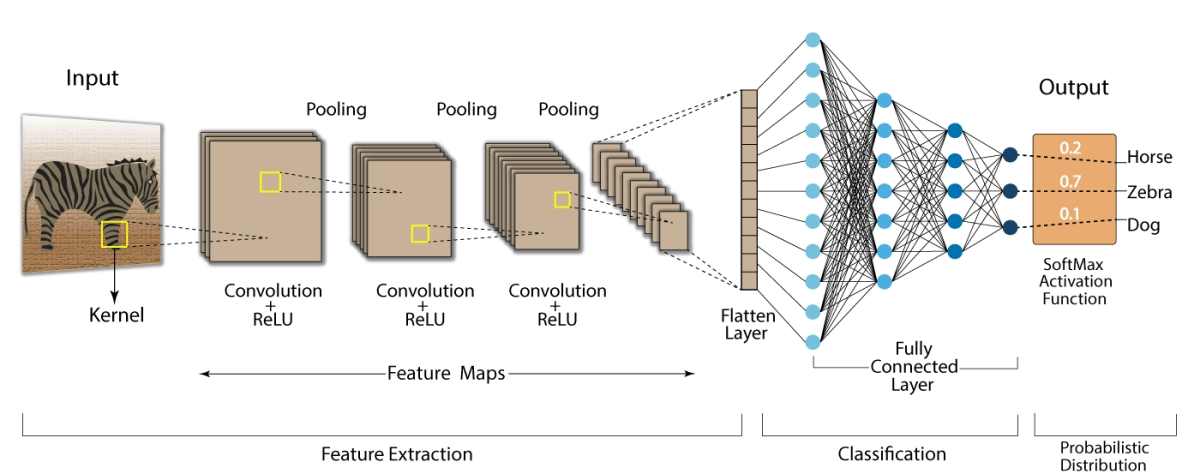
\includegraphics[height=05cm]{ch2-CNN_archi-01.jpg}
	\caption{Réseau de neurones convolutifs}
\label{fig:CNN}
\end{figure}

\textbf{1- Couche de convolution:} cette couche applique des opérations de convolution sur les entrées, à l'aide des filtres, pour extraire des caractéristiques locales et spatiales des données. Chaque filtre est une matrice de poids avec une taille bien définie, qui est appliquée à une fenêtre glissante de l'entrée. Pendant la convolution, les poids du filtre sont multipliés avec les valeurs de la fenêtre d'entrée, puis les produits sont sommés pour obtenir une seule valeur. Ce processus est répété pour chaque position de la fenêtre glissante, couvrant ainsi l'ensemble de l'entrée. Les résultats de ces opérations de convolution sont rassemblés dans une carte d'activation appelée carte des caractéristiques ou feature map.
la figure \ref{fig:convolution} montre l'opération de convolution sur une matrice en entrée \cite{cnn_Agronomy86}.

\begin{figure}[H]
	\centering
	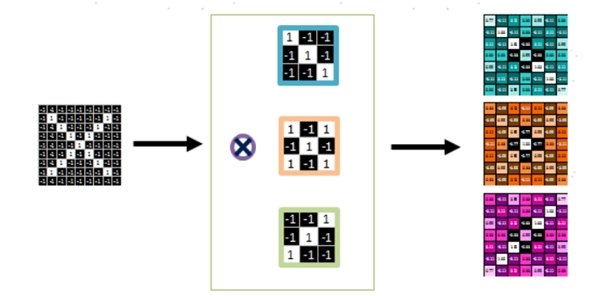
\includegraphics[height=05cm]{ch2-cnn-Couche de convolution.jpg}
	\caption{Convolution d'une image}
 \label{fig:convolution}
\end{figure}

\textbf{2- Couche de mise en commun (pooling) :} selon la figure \ref{fig:pooling}, la couche pooling consiste à diminuer la dimensionnalité des caractéristiques extraites par la couche de convolution d'un CNN. Son objectif est de conserver les informations les plus importantes tout en réduisant le nombre de paramètres et en évitant le sur-apprentissage. L'opération de mise en commun se fait en utilisant une fenêtre (généralement de taille 2x2 pixels) qui se déplace sur les cartes des caractéristiques. À chaque position de la fenêtre, la valeur maximale (ou parfois la moyenne) des pixels couverts par la fenêtre est conservée, tandis que les autres valeurs sont ignorées \cite{makina-corpus}.

\begin{figure}[H]
	\centering
	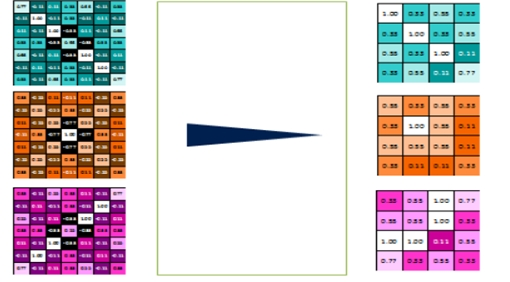
\includegraphics[height=05cm]{ch2-cnn-pooling.jpg}
	\caption{Opération de mise en commun}
 \label{fig:pooling}
\end{figure}

\textbf{3- couche entièrement connectée(dense ou fully connected en anglais):}
joue un rôle fondamental au sein des CNN. Chaque neurone au sein de cette couche est connecté à tous les neurones de la couche précédente, avec des poids définis pour chaque connexion. Les entrées sont soumises à un processus de pondération et de sommation, suivi de l'application d'une fonction d'activation non linéaire telle que la sigmoïde, la ReLU (Rectified Linear Activation), la tangente hyperbolique (tanh), et autres. Cette fonction d'activation permet au réseau de saisir les relations complexes entre les données en introduisant des seuils et des non-linéarités dans les calculs. Les couches entièrement connectées sont fréquemment positionnées vers la fin d'un réseau de neurones afin de fusionner et combiner les caractéristiques apprises des couches précédentes, en vue de produire en fin de compte une sortie finale correspondant aux prédictions du modèle, telles que la classification d'une image ou la prédiction d'une valeur numérique, par exemple \cite{makina-corpus}..Et c'est ce qui est représenté sur la figure \ref{fig:fully},
\begin{figure}[H]
	\centering
	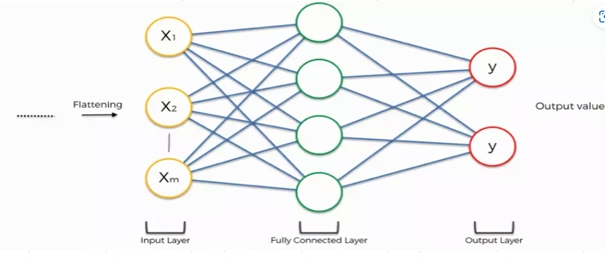
\includegraphics[height=05cm]{ch2-cnn-full connection.jpg}
	\caption{Couche entièrement connectée}
 \label{fig:fully}
\end{figure}

%-- https://datascientest.com/convolutional-neural-network
%   https://makina-corpus.com/sig-webmapping/extraction-dobjets-pour-la-cartographie-par-deep-learning-choix-du-modele

\subsection{Architectures CNN}
Un éventail d'architectures majeures a été développé, parmi lesquelles nous pouvons mentionner :
\begin{outline}
\1 LeNet: développé par Yann LeCun en 1998, a été l'un des premiers réseaux de neurones convolutifs à gagner en popularité. Il a été spécifiquement conçu pour la reconnaissance de chiffres manuscrits. Cette architecture comportait plusieurs couches de convolution et de sous-échantillonnage, ainsi que des couches entièrement connectées à la fin. Bien que relativement simple par rapport aux architectures modernes, LeNet a ouvert la voie à la compréhension de la puissance des CNN dans la vision par ordinateur \cite{vitalflux2023different}.

\1 AlexNet: présenté en 2012 par Alex Krizhevsky et son équipe, a marqué un tournant dans l'utilisation des CNN pour la classification d'images. Il a remporté le concours ImageNet en 2012 en obtenant une précision remarquable. AlexNet a introduit l'utilisation répandue de la fonction d'activation ReLU et a montré comment l'augmentation des données d'entraînement pouvait grandement améliorer les performances du modèle. Cette architecture comportait des couches de convolution, de pooling et des couches entièrement connectées, créant un précédent pour les CNN modernes \cite{vitalflux2023different}.

\1 VGGNet : proposé en 2014 par Simonyan et Zisserman, a été remarquable pour sa profondeur. Cette architecture avait une structure très uniforme avec plusieurs couches de convolution de taille 3x3, suivies de couches de pooling, et enfin de couches entièrement connectées. Bien que VGGNet soit plus profond que les modèles précédents, sa simplicité a permis de mieux comprendre comment la profondeur du réseau peut influencer la performance \cite{analyticsvidhya2019vggnet}.

\1 GoogLeNet (Inception) : également connu sous le nom d'Inception, est une architecture révolutionnaire introduite par Szegedy et son équipe en 2014. Elle a introduit le concept de modules Inception, où plusieurs filtres de différentes tailles sont appliqués en parallèle pour capturer des caractéristiques à différentes échelles. Cela a permis d'obtenir des performances de pointe tout en maintenant une complexité relativement faible, grâce à l'utilisation efficace des opérations de convolution \cite{medium-article}.

\1 ResNet (Residual Network) : L'architecture ResNet, présentée en 2015 par Kaiming He et ses collaborateurs, a abordé le problème du "vanishing gradient" en introduisant les blocs résiduels. Ces blocs utilisaient des connexions de saut (skip connections) pour ajouter directement les sorties des couches précédentes aux couches suivantes. Cela a permis la formation de réseaux extrêmement profonds sans subir de dégradation de performance due au problème du gradient. Les ResNets ont ouvert la voie à la création de modèles encore plus profonds et performants \cite{geeksforgeeks-resnet}.
\end{outline}

Chacune de ces architectures a contribué de manière significative à l'avancement des CNN en introduisant des idées novatrices pour la capture de caractéristiques et la gestion de la profondeur. Elles occupent une place essentielle dans le domaine de la vision par ordinateur en permettant l'extraction automatique de caractéristiques visuelles à partir de données complexes, particulièrement dans des domaines tels que la détection d'objets.

Le tableau \ref{tab:my-table} illustre une série de modèles CNN qui sont intégrés automatiquement dans le framework Keras, ainsi que les caractéristiques respectives: taille (en MB), exactitude top-1, exactitude top-5, nombre de paramètres, profondeur du modèle et temps d'exécutionen en ms (CPU/ GPU) \cite{ch2_KerasApp87}.

\begin{table}[h]
\centering
\caption{Modèles CNN prédéfinis dans le framework Keras \cite{ch2_KerasApp87}.}
\label{tab:my-table}
\resizebox{\columnwidth}{!}
{
    \begin{tabular}{|l|l|l|l|l|l|p{2cm}|p{2cm}|}
    \hline
    Modèle & Taille & Exactitude top-1 & Exactitude top-5  & Paramètres & Profondeur & Temps (CPU)(MS) & Temps (GPU)(MS) \\
    \hline
    Xception          & 88     & 79.00\% & 94.50\% & 22.9M  & 81  & 109.4  & 8.1  \\
    VGG16             & 528    & 71.30\% & 90.10\% & 138.4M & 16  & 69.5   & 4.2  \\
    VGG19             & 549    & 71.30\% & 90.00\% & 143.7M & 19  & 84.8   & 4.4  \\
    ResNet50          & 98     & 74.90\% & 92.10\% & 25.6M  & 107 & 58.2   & 4.6  \\
    ResNet50V2        & 98     & 76.00\% & 93.00\% & 25.6M  & 103 & 45.6   & 4.4  \\
    ResNet101         & 171    & 76.40\% & 92.80\% & 44.7M  & 209 & 89.6   & 5.2  \\
    ResNet101V2       & 171    & 77.20\% & 93.80\% & 44.7M  & 205 & 72.7   & 5.4  \\
    ResNet152         & 232    & 76.60\% & 93.10\% & 60.4M  & 311 & 127.4  & 6.5  \\
    ResNet152V2       & 232    & 78.00\% & 94.20\% & 60.4M  & 307 & 107.5  & 6.6  \\
    EfficientNetB0    & 29     & 77.10\% & 93.30\% & 5.3M   & 132 & 46     & 4.9  \\
    \hline  
    \end{tabular}   
}
\end{table}

\subsection{Apprentissage par transfert}

L'apprentissage par transfert est une approche dans le domaine de l'apprentissage automatique où les connaissances et les modèles acquis lors de la résolution d'une tâche sont transférés pour aider à résoudre une tâche similaire ou connexe. Plutôt que de construire un modèle à partir de zéro pour chaque nouvelle tâche, on utilise les informations déjà apprises dans le cadre d'une tâche précédente pour accélérer et améliorer l'apprentissage d'une nouvelle tâche \cite{Transfer_Transfer32}.\\
Les avantages de l'apprentissage par transfert sont nombreux, notamment la réduction du temps et des ressources nécessaires pour entraîner un modèle, une meilleure généralisation sur de petits ensembles de données, et la possibilité d'appliquer des connaissances d'un domaine à un autre \cite{Transfer_WhatIsTr80}.\\
Cependant, le succès de l'apprentissage par transfert dépend de la similitude entre les tâches sources et cibles. Si les tâches sont trop différentes, le transfert peut ne pas être aussi efficace. Les techniques d'apprentissage par transfert incluent le transfert de caractéristiques (où les couches basses d'un modèle préalablement formé sont utilisées comme extracteurs de caractéristiques), le transfert de connaissances (où des connaissances spécifiques à une tâche sont transférées), et l'adaptation fine (où un modèle préalablement formé est ajusté pour mieux s'adapter à une tâche spécifique) \cite{Transfer_Transfer45}.

\section{ Vision par ordinateur}

La vision par ordinateur constitue un champ interdisciplinaire qui fait partie de l'intelligence artificielle. Il se concentre sur la conception d'ordinateurs capables d'acquérir une compréhension avancée à partir de données visuelles, telles que des images ou des vidéos numériques. D'un point de vue d'ingénierie, son objectif est d'automatiser les fonctions réalisables par le système visuel humain \cite{Vision_par_ordinateur_Computer61}. 

\begin{figure}[H]
	\centering
	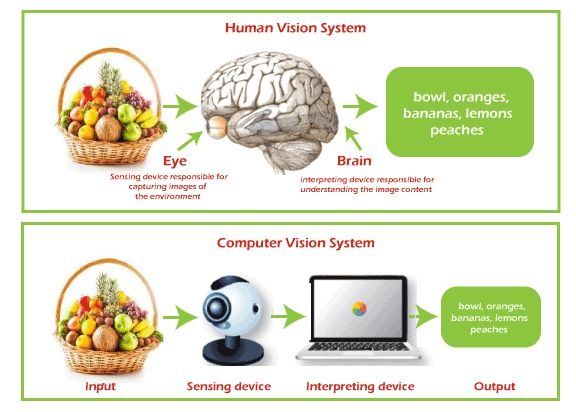
\includegraphics[height=07cm]{ch2-process_cv.jpg}
	\caption{Processus de la vision par ordinateur}
    \label{ch2-process_cv}
\end{figure}

Son évolution, grâce à l'apprentissage automatique et profond, a été marquée par des progrès significatifs. Depuis les années 1960, avec les premiers programmes de reconnaissance de caractères imprimés, la vision par ordinateur est passée d'algorithmes basés sur des règles à des méthodes traitant des tâches complexes. L'arrivée de l'apprentissage automatique dans les années 1990 a ouvert de nouvelles perspectives, permettant aux ordinateurs d'apprendre à partir de données plutôt que de règles prédéfinies. Ceci a amélioré leur performance dans différents problèmes notamment dans la détection d'objets. La figure \ref{ch2-process_cv} présente la relation entre l'intelligence artificielle et ses divers domaines en lien avec la vision par ordinateur.

\subsection{Techniques de la vision par ordinateur}
Les techniques de la vision par ordinateur sont des méthodes et des approches utilisées pour traiter et analyser des données visuelles, notamment des images et des vidéos \cite{javatpoint2023computer}. Certaines des techniques les plus importantes et couramment utilisées dans ce domaine comprennent Et montré sur la figure \ref{fig:ch2-Techniques_cv}:

\begin{itemize}
    \item  \textbf{Classification d'images} : Prédire la classe d'une image en fonction de son contenu visuel.
    \item  \textbf{Détection d'objets} : Localiser et identifier la présence d'objets spécifiques dans une image.
    \item  \textbf{Détection des points d'intérêt} : Identifier et localiser de caractéristiques significatives (points, coins, blobs, ... etc.) dans une image.
    \item  \textbf{Segmentation d'objets (ou sémantique)} : Diviser une image en régions pour identifier les parties spécifiques des objets.
    \item  \textbf{Reconnaissance de formes} : Identifier des motifs spécifiques dans les données visuelles.
    \item  \textbf{Suivi d'objets} : Suivre les mouvements et les interactions des objets dans une séquence d'images.
    \item  \textbf{Segmentation d'instances} : Identifier et séparer chaque instance d'objet distincte au sein d'une image.
    \item  \textbf{Reconstruction 3D} : Créer des modèles tridimensionnels à partir d'images bidimensionnelles.
    \item  \textbf{Estimation de mouvement} : Déterminer les mouvements et les déplacements des objets dans une séquence d'images.

Ces techniques sont largement utilisées pour résoudre une variété de problèmes de vision par ordinateur, allant de l'analyse d'images médicales à la navigation autonome des véhicules.
\end{itemize}

\begin{figure}[H]
	\centering
	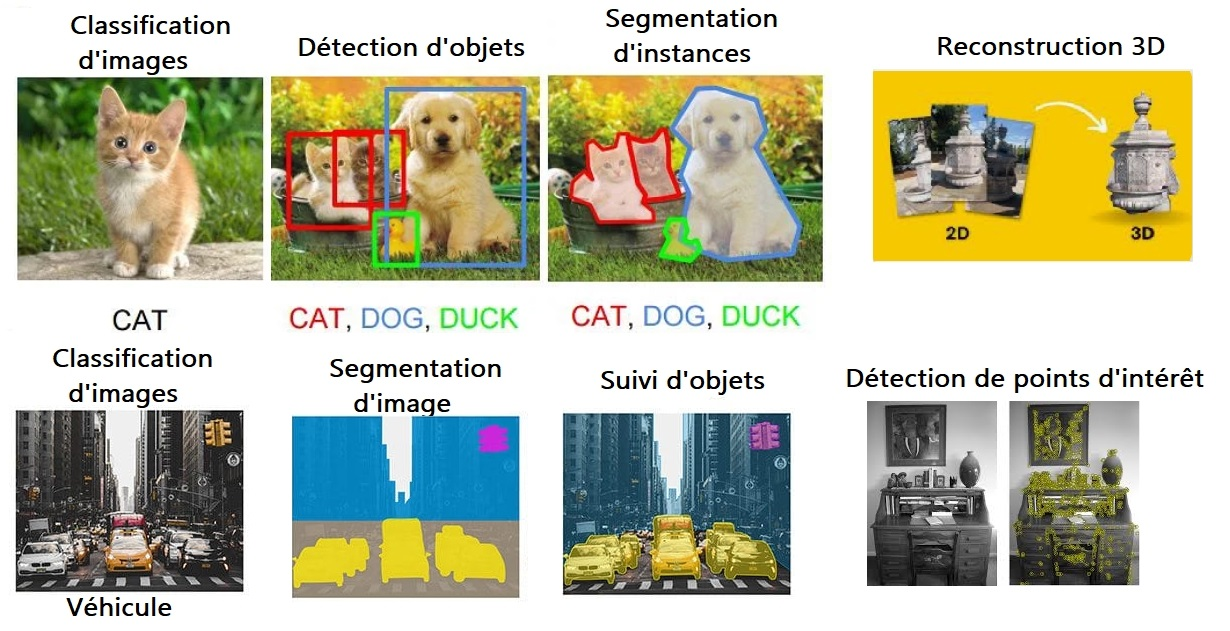
\includegraphics[height=08cm]{ch2-Techniques_cv.jpg}
	\caption{Techniques de la vision par ordinateur \cite{simplilearn2023computer}}
    \label{fig:ch2-Techniques_cv}
\end{figure}

\subsection{Applications de la vision par ordinateur }

La vision par ordinateur est utilisée dans des domaines variés \cite{simplilearn2023computer}, notamment:

\subsubsection{ Véhicules autonomes }
Grâce à des caméras et des algorithmes de vision, les véhicules autonomes peuvent percevoir leur environnement, détecter les bords de la route, les panneaux de signalisation, autres véhicules, obstacles et piétons, leur permettant de naviguer en toute sécurité \cite{simplilearn2023computer}.

\subsubsection{Reconnaissance faciale }
Les algorithmes de reconnaissance faciale utilisent la vision par ordinateur pour identifier des individus dans des images. Ils identifient les caractéristiques du visage, les comparant à des profils enregistrés. Cela a des applications allant de la vérification d'identité sur les appareils électroniques grand public à l'application dans les réseaux sociaux et les forces de l'ordre \cite{simplilearn2023computer}.

\subsubsection{Réalité augmentée et mixte }
La vision par ordinateur est essentielle pour la réalité augmentée, où des éléments numériques sont superposés sur le monde réel via des caméras. Ces technologies utilisent la vision par ordinateur pour reconnaître les surfaces et positionner correctement les éléments virtuels dans l'environnement réel \cite{simplilearn2023computer}.

\subsubsection{Santé }
La vision par ordinateur a transformé le secteur médical en automatisant des tâches telles que la détection de problèmes dermatologiques ou l'analyse d'images médicales comme les radiographies et les IRM, ce qui accélère les diagnostics et les traitements \cite{simplilearn2023computer}.

\section{Algorithmes de détection d'objets}

La détection d'objets au sein d'images ou de séquences d'images constitue une application cruciale de la vision par ordinateur. Cette technologie trouve des applications variées, telles que la surveillance, l'automatisation industrielle, la robotique, la sécurité et les véhicules autonomes, entre autres. Pour accomplir cette tâche complexe, une gamme d'algorithmes est utilisée. Ces méthodes peuvent être regroupées en deux catégories principales : les détecteurs à un seul niveau et les détecteurs à deux niveaux, en fonction du schéma illustré dans la figure \ref{ch2-oneStage-twoStage-01}.

\begin{figure}[H]
	\centering
	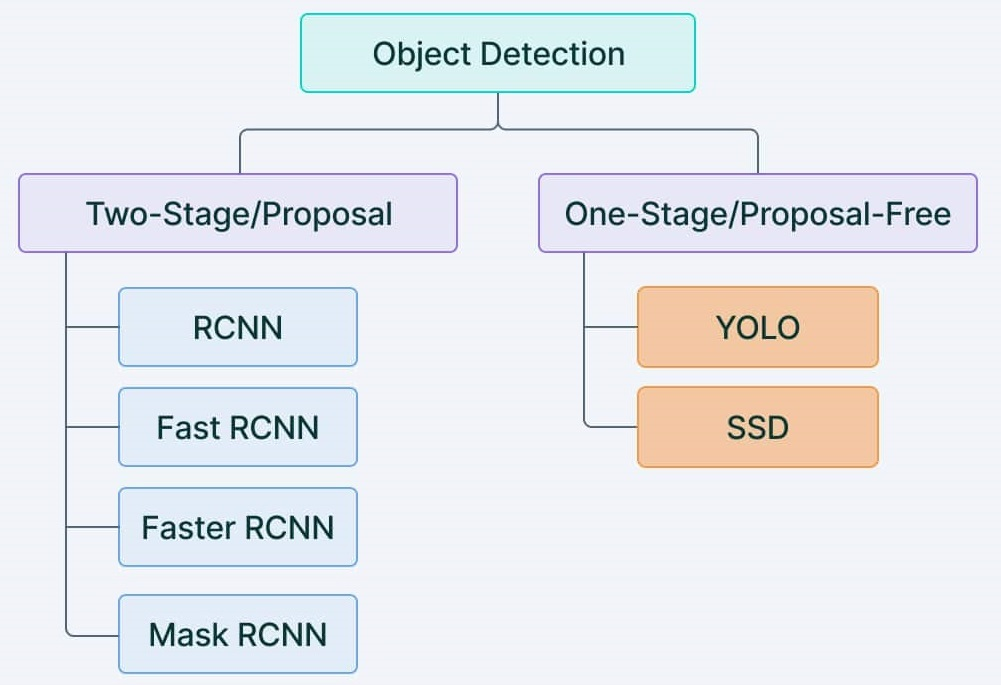
\includegraphics[height=08cm]{ch2-oneStage-twoStage-01.jpg}
	\caption{Classification des algorithmes de détection d'objets }
 \label{ch2-oneStage-twoStage-01}
\end{figure}

\subsubsection{Détecteurs d'objets à deux niveaux}
La  détection d'objets à deux niveaux (two-shot object detection ) fait référence à une approche en deux étapes pour détecter et localiser des objets au sein d'une image \cite{ch2_The5Comp69}.
Dans un détecteur d'objets à deux niveaux, la détection se fait en deux étapes distinctes :
\begin{itemize}
    \item [(1)] Génération de propositions (régions d'intérêt) : Dans la première étape, le modèle génère des régions d'intérêt qui pourraient potentiellement contenir des objets. Ces régions sont extraites en utilisant des techniques telles que les régions de haute probabilité basées sur des caractéristiques visuelles. Cela réduit le nombre de régions à examiner plus en détail dans la prochaine étape.
    \item [(2)] Classification et localisation : Dans la deuxième étape, les régions d'intérêt générées sont soumises à des modèles de classification et de localisation. Le modèle classe chaque région comme contenant un certain type d'objet ou non, et ajuste également les boîtes englobantes autour de ces objets.
\end{itemize}

Cette approche offre plus de précision mais potentiellement plus lente.

\subsubsection{Détecteurs d'objets à un niveau}  
Dans la détection d'objets à un niveau (single-shot object detection), la détection et la classification des objets sont effectuées simultanément en une seule étape, sans nécessiter une étape distincte de génération de propositions \cite{ch2_The5Comp69}.

Dans les détecteurs d'objets à un seul niveau, l'algorithme prédit directement les boîtes englobantes des objets ainsi que leurs étiquettes de classe correspondantes. Cela simplifie le processus en éliminant le besoin de générer d'abord des propositions de région, puis de les classifier et de les affiner comme dans les détecteurs à deux niveaux. \\
Bien que les détecteurs à un seul niveau offrent des avantages en termes de vitesse, ils peuvent parfois sacrifier une certaine précision par rapport aux détecteurs à deux niveaux en raison de la nature directe et simultanée de leurs prédictions \cite{ch2_The5Comp69}.\\

\subsection{RCNN}
RCNN (Region-based Convolutional Neural Network) a été l'une des premières approches populaires pour la détection d'objets basée sur CNN. Il fonctionne selon les étapes suivantes: 
\begin{itemize}
    \item Proposition de régions : La première étape de RCNN consiste à générer un ensemble de régions d'intérêt (ROIs) dans une image. Cela se fait généralement à l'aide d'une méthode de propositions de régions, telle que selective search. Cette dernière parcourt l'image pour identifier des régions qui semblent contenir des objets et les propose comme ROIs. Ces ROIs peuvent être de différentes tailles et formes \cite{ch2_The5Comp69}.
    \item Extraction de caractéristiques : Une fois que les ROIs ont été identifiées, chaque ROI est découpée de l'image originale et redimensionnée pour avoir une taille fixe. Ensuite, un CNN pré-entraîné, comme VGG16 ou autre, est utilisé pour extraire des caractéristiques de chaque ROI. Le CNN transforme l'image de la ROI en un vecteur de caractéristiques de dimension fixe \cite{ch2_The5Comp69}.
    \item Classification : Les vecteurs de caractéristiques extraits de chaque ROI sont ensuite introduits dans un classifier. Ce dernier est généralement une couche entièrement connectée qui attribue une classe (parmi les classes d'objets prédéfinies) à chaque ROI. Il s'agit de déterminer quelle est la nature de l'objet contenu dans la ROI \cite{ch2_The5Comp69}.
    \item Régression des boîtes de délimitation : En plus de la classification, RCNN effectue également une régression des boîtes de délimitation autour des objets. Cela signifie qu'il ajuste les coordonnées des boîtes englobantes autour des objets pour les rendre plus précises \cite{ch2_The5Comp69}.
    \item Non-maximum suppression : Après avoir effectué la classification et la régression, RCNN applique une méthode connue sous le nom de suppression des non-maxima (NMS) pour éliminer les détections redondantes ou peu fiables, assurant ainsi que chaque objet n'est détecté qu'une seule fois. Cette technique repose sur la mesure "IoU" (Intersection Over Union) \cite{ch2_The5Comp69}.
\end{itemize}
Cependant, une limitation majeure de RCNN est sa lenteur en raison du traitement indépendant des ROIs, ce qui a conduit au développement de versions plus rapides et efficaces telles que Fast R-CNN et Faster R-CNN.


\subsection{Fast R-CNN} 
Fast R-CNN est une amélioration significative par rapport à RCNN en termes d'efficacité \cite{ren2015fasterarxiv}. Il élimine la nécessité de traiter chaque ROI indépendamment. Au lieu de cela, il utilise une seule passe CNN sur l'image entière pour extraire des caractéristiques. Les ROIs sont ensuite alignées avec les caractéristiques extraites de l'image globale.
Fast R-CNN a été plus rapide que RCNN car il évite de répéter le calcul coûteux des caractéristiques pour chaque ROI.
Fast R-CNN se distingue par sa rapidité par rapport à RCNN, car il élimine la nécessité de recalculer les caractéristiques  pour chaque ROI \cite{ch2_The5Comp69}.


\subsection{Faster R-CNN}
Faster R-CNN est une autre amélioration majeure par rapport à Fast R-CNN. Selon la figure \ref{FasterRCNN}, Faster R-CNN (Faster Region-based Convolutional Neural Network) \cite{ren2015faster} se compose de plusieurs composants clés qui travaillent ensemble pour effectuer la détection d'objets :
\begin{itemize}
    \item CNN: l'architecture commence par un réseau neuronal convolutif de base, tel que VGG16 ou des modèles similaires. Ce réseau extrait des caractéristiques de l'image d'entrée, créant ainsi une carte de caractéristiques qui encode des informations visuelles importantes \cite{ch2_The5Comp69}.
    \item Réseau de proposition de régions (RPN) : est intégré au réseau neuronal de base et génère directement des propositions de régions à partir de la carte de caractéristiques. Ces propositions sont des régions potentielles où des objets pourraient être présents. Le RPN suggère des régions en fonction de boîtes d'ancrage (boîtes prédéfinies de différentes tailles et rapports d'aspect) et prédit la probabilité de présence d'un objet ainsi que les ajustements à apporter aux boîtes d'ancrage pour bien encadrer les objets \cite{ch2_The5Comp69}.
    \item RoI pooling (ou RoI Align) : les régions proposées par le RPN sont alignées sur une taille et une forme fixes (par exemple, 7x7) à l'aide de RoI pooling ou RoI align. Cette étape garantit que les caractéristiques des régions ont une taille cohérente, ce qui est nécessaire pour les tâches de classification et de régression qui suivent \cite{ch2_The5Comp69}.
    \item Tête de détection (classification et régression des boîtes englobantes): les caractéristiques des régions alignées sont introduites dans une tête de classification, qui prédit la probabilité que chaque région proposée contienne différentes classes d'objets. Cette classification est généralement effectuée à l'aide de couches entièrement connectées ou de convolutions 1x1.
    De plus, les mêmes caractéristiques passent par la tête de régression des boîtes englobantes, qui ajuste les paramètres des boîtes d'ancrage pour obtenir une adaptation précise des boîtes englobantes des objets détectés \cite{ch2_The5Comp69}.  
\end{itemize}

\begin{figure}[H]
	\centering
	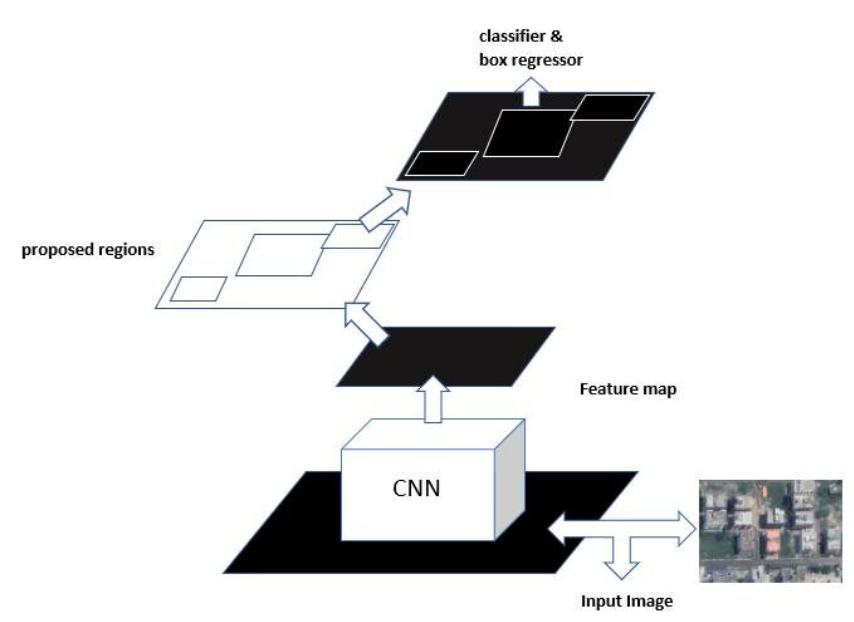
\includegraphics[height=07cm]{img/Faster-R-CNN2.png}
	\caption{L'architecture du Faster R-CNN}
 \label{FasterRCNN}
\end{figure}

\subsection{SSD}
Le SSD (Single Shot MutiBox Detector) est un détecteur capable de détecter plusieurs objets à différentes échelles en une seule étape, comme illustré dans la figure \ref{SSD}. Il réalise cette détection en prédisant des boîtes d'ancrage de différentes tailles et proportions \cite{liu2016ssd}. L'architecture SSD  est composée de plusieurs composants, notamment :
\begin{itemize}
    \item Backbone convolutif : SSD utilise un réseau de neurones convolutifs profonds pré-entraîné, généralement basé sur des architectures telles que VGG16 , comme base pour extraire des caractéristiques d'image. Ce réseau sert de "backbone" pour le modèle \cite{ch2_The5Comp69}.
    \item Pyramide de caractéristiques (feature pyramid) : SSD construit une pyramide de caractéristiques en ajoutant des couches de convolution supplémentaires au réseau de base. Ces couches sont conçues pour capturer des informations à différentes échelles spatiales, ce qui permet de détecter des objets de différentes tailles \cite{ch2_The5Comp69}.
    \item Boîtes d'ancrage (anchor boxes) : Pour chaque cellule de la pyramide de caractéristiques, SSD prédit un ensemble de boîtes d'ancrage de différentes tailles et rapports (aspect ratios). Ces boîtes d'ancrage servent de points de référence pour la détection d'objets \cite{ch2_The5Comp69}.
    \item Prédiction des boîtes multibox : Pour chaque boîte d'ancrage, SSD prédit à la fois les décalages (offsets) par rapport à la boîte d'ancrage et les scores de classification pour chaque classe d'objet. Cela signifie qu'il prédit à la fois où se trouve l'objet par rapport à la boîte d'ancrage et quelle est la classe de l'objet.
    Après la prédiction des boîtes MultiBox, SSD applique une étape de non-maximum suppression pour éliminer les détections redondantes et ne conserver que les détections les plus fiables \cite{ch2_The5Comp69}.
\end{itemize}

 
Pour l'apprentissage du modèle SSD, il utilise une fonction de perte qui prend en compte à la fois la classification (score de confiance) et la régression (décalage par rapport aux boîtes d'ancrage) pour entraîner le modèle. Cela inclut généralement une perte de classification et une perte de régression.
   
L'architecture SSD est très efficace pour la détection d'objets en temps réel. 

\begin{figure}[H]
	\centering
	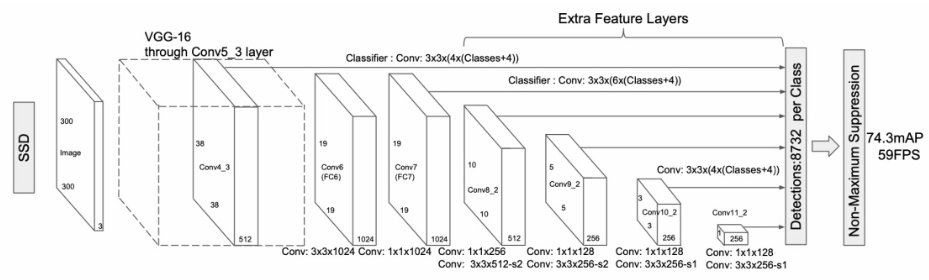
\includegraphics[height=5cm]{ch2-SSD.png}
	\caption{L'architecture du détecteur SSD}
    \label{SSD}
\end{figure}


\subsection{YOLO}
L'algorithme YOLO (You Only Look Once) représente une avancée révolutionnaire en matière de détection d'objets, car il analyse l'intégralité d'une image en une seule itération au travers un CNN \cite{redmon2016yolo}. Son architecture se décompose comme suit :
\begin{itemize}
    \item Couche d'entrée : L'image d'entrée est divisée en une grille de cellules. Chaque cellule est responsable de la détection des objets dans sa région.
    \item  Réseau "backbone": YOLO utilise un CNN pour extraire des caractéristiques importantes de l'image. Il prend en compte l'ensemble de la grille et capture des informations à différentes échelles spatiales.
    \item "Neck": est habituellement constitué de couches de convolution supplémentaires visant à 
    agréger les caractéristiques extraites de la grille à différentes résolutions spatiales et effectue des opérations de fusion pour intégrer des informations provenant de différentes échelles.
    \item Tête de prédiction: comprend des couches de convolution spécifiques pour produire les prédictions. Pour chaque grille, YOLO prédit un certain nombre de boîtes englobantes et les probabilités associées à différentes classes d'objets. Chaque boîte englobante est caractérisée par ses coordonnées (coordonnées x et y de son centre, largeur et hauteur) et les probabilités de classe correspondantes.
    
    Après les prédictions, YOLO applique une étape de non-maximum suppression pour éliminer les boîtes englobantes redondantes et ne conserver que les détections les plus fiables.
\end{itemize}

L'architecture du modèle \cite{ch2_YOLOdéte70} se compose de 24 couches convolutives pour extraire les cartes de caractéristiques suivies de 2 couches entièrement connectées pour réaliser la détection d'objets, comme illustré dans la figure \ref{YOLOarc}.
\begin{figure}[H]
	\centering
	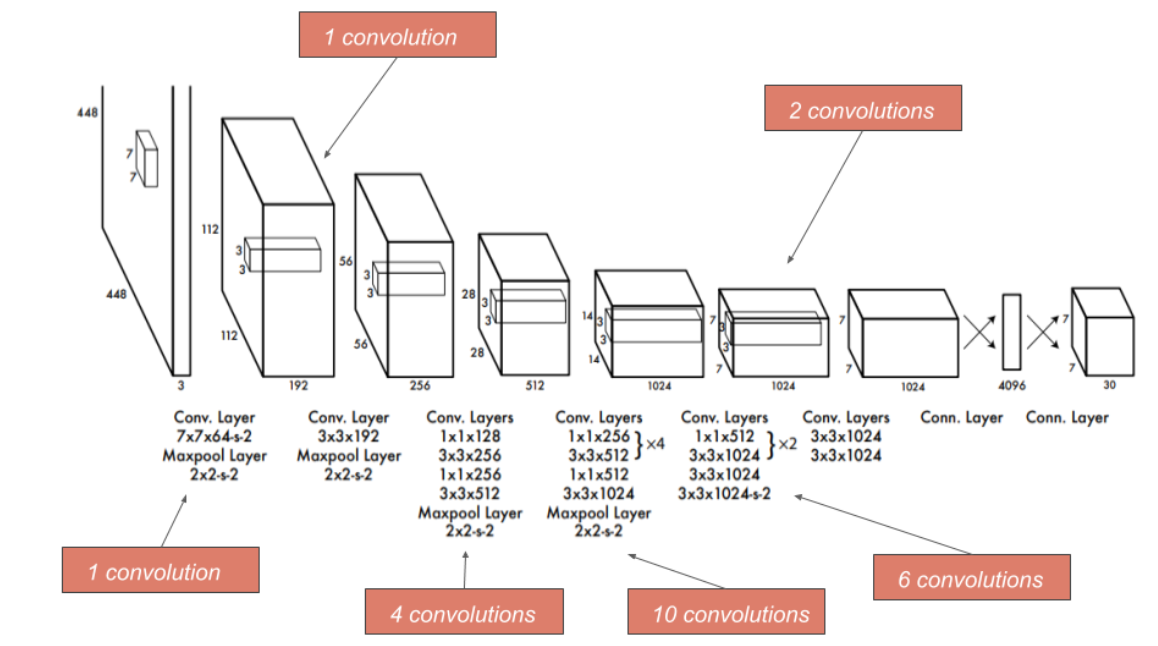
\includegraphics[height=8cm]{ch2-yolo_arch.png}
	\caption{L'architecture du détecteur YOLO}
 \label{YOLOarc}
\end{figure}

YOLO est connu pour sa rapidité et sa précision, car il évite la nécessité de générer des propositions de régions ou de passer plusieurs fois à travers le réseau. Il est couramment utilisé dans des applications telles que la détection d'objets en temps réel, la surveillance vidéo, la conduite autonome et bien d'autres.
\\
Plusieurs versions de YOLO \cite{AGuideto8}ont été développées pour améliorer les performances de la détection, notamment:
YOLOv1 (Juin, 2015),
YOLOv2 (Dec, 2016),
YOLOv3 (Avr, 2018),
YOLOv4 (Avr, 2020),
YOLOv5 (Mai, 2020),
YOLOv6,
YOLOv7,
YOLOv8.

\begin{figure}[H]
	\centering
	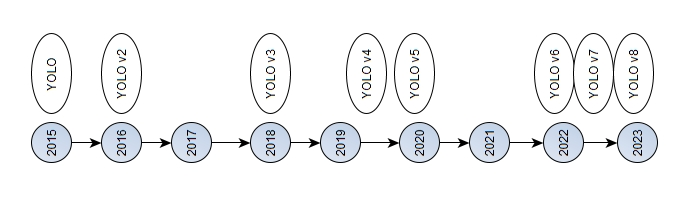
\includegraphics[height=05cm]{ch2-cnn-yolo-all.jpg}
	\caption{Les versions de l'algorithme YOLO}
 \label{YOLO}
\end{figure}

Les principales améliorations de YOLOv8 \footnote{\url{https://blog.roboflow.com/whats-new-in-yolov8/}} incluent l'introduction d'un nouveau réseau fédérateur, une tête divisée innovante sans ancrage, ainsi que de nouvelles fonctions de perte. Ces améliorations permettent à YOLOv8 d'obtenir des performances exceptionnelles tout en conservant une empreinte mémoire réduite et une vitesse d'entraînement remarquable.\\
D'après l'architecture illustrée dans la figure \ref{fig:ch2-yolov8_arch}, ce réseau requiert une image d'entrée de forme carrée, avec une longueur de côté qui doit être un multiple de 32. La forme de l'entrée est couramment représentée comme (3, imgsz, imgsz), où :

\begin{outline}
    \1 "3" indique qu'il y a trois canaux de couleur (rouge, vert, bleu) dans l'image.
    \1 "imgsz" représente la largeur (w) et la hauteur(h) de l'image, qui sont identiques (h=w).
\end{outline}
La sortie du réseau YOLOv8 est représentée sous la forme d'une matrice avec une largeur et une hauteur.
\begin{equation}
\textbf{Largeur} = \text{nombre de classes} + 4
\end{equation}
La hauteur de cette matrice dépend de la taille de l'image d'entrée et est calculée de la manière suivante:
\begin{equation}
\textbf{Hauteur} = 
\left(\frac{{\text{imgsz}}}{{32}}\right)^2 + \left(\frac{{\text{imgsz}}}{{16}}\right)^2 + \left(\frac{{\text{imgsz}}}{{8}}\right)^2
\end{equation}
Chaque ligne de cette matrice représente un objet et est structurée comme suit : [x\_centre de l'objet, y\_centre de l'objet, hauteur, largeur, Score prédiction de classe 1, Score prédiction de classe 2, ...,Score prédiction de classe  N].

\begin{figure}[H]
	\centering
	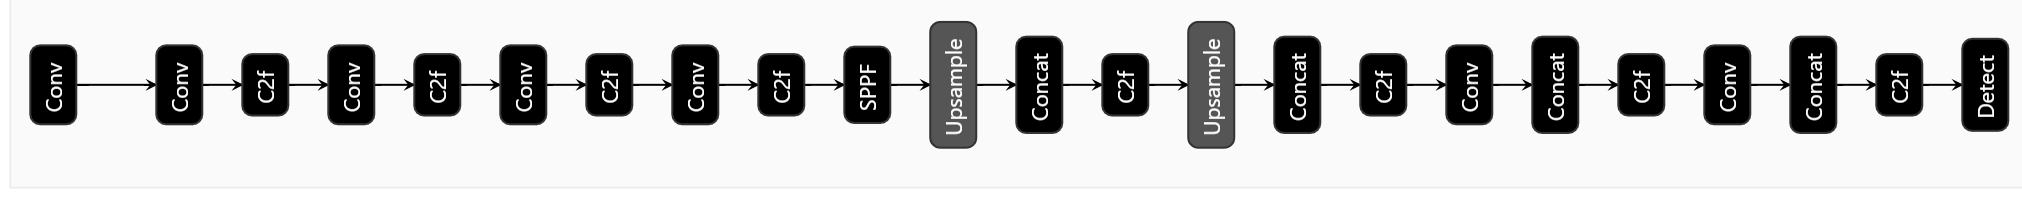
\includegraphics[width=17cm]{ch2-yolov8_arch.png}
	\caption{Architecture du YOLOv8}
    \label{fig:ch2-yolov8_arch}
\end{figure}
% https://github.com/lutzroeder/netron/
% Un programme a été utilisé pour créer ce graphique en utilisant le fichier de poids généré par  yolov8 poid

Il existe cinq extensions du modèle YOLOv8 : YOLOv8n (nano), YOLOv8s (small),YOLOv8m (medium), YOLOv8l (large), YOLOX (eXtra large). YOLOv8 Nano est le plus rapide et le plus petit, tandis que YOLOv8 Extra Large (YOLOv8x) est le plus précis mais aussi le plus lent parmi eux.



\section{Reconnaissance optique de caractères}

L'OCR, ou Optical Character Recognition en anglais (Reconnaissance Optique de Caractères en français), est une technologie qui permet de convertir du texte manuscrit ou imprimé, que ce soit sur du papier ou une image, en texte éditable sur un ordinateur. Cette conversion est réalisée grâce à des ordinateurs et des logiciels spécialement conçus pour analyser les images, extraire les caractères, chiffres et mots, puis les transformer en texte que l'on peut modifier et manipuler \cite{ch2_ocr_definitionxcs}.

Pour illustrer cela, la figure \ref{fig:ch2-ocr_info} montre une image contenant deux mots. Grâce à l'OCR, cette image a été traitée pour produire un texte que l'on peut éditer.

\begin{figure}[H]
	\centering
	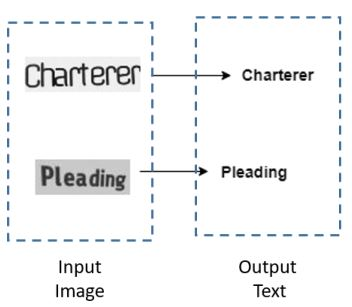
\includegraphics[height=5cm]{ch2-ocr_info.JPG}
	\caption{Reconnaissance optique de caractères}
    \label{fig:ch2-ocr_info}
\end{figure}
En général, le processus d'OCR comprend les étapes suivantes:
\begin{itemize}
    \item [-] Acquisition de l'image : Tout d'abord, une image contenant du texte est acquise à l'aide d'un scanner, d'un appareil photo numérique ou d'un autre moyen de capture d'images. L'image peut contenir du texte imprimé, manuscrit, ou une combinaison des deux.
    \item [-] Prétraitement : L'image capturée peut contenir diverses imperfections telles que des taches, des plis de papier, ou un mauvais contraste. Avant d'effectuer la reconnaissance optique de caractères, l'image est soumise à un prétraitement pour améliorer sa qualité. Cela peut inclure le redressement de l'image, la correction de la luminosité et du contraste, et la suppression du bruit.
    \item [-] Segmentation des caractères : Dans cette étape, l'image est analysée pour séparer les caractères individuels, les mots et les lignes de texte. Cela permet de délimiter clairement chaque élément textuel, ce qui facilite leur traitement ultérieur.
    \item [-] Reconnaissance des caractères : La partie centrale de l'OCR consiste à identifier les caractères individuels présents dans l'image. Cela se fait en comparant les formes des caractères extraits de l'image avec un ensemble de caractères connus. Les algorithmes d'apprentissage automatique, tels que les réseaux neuronaux, sont couramment utilisés pour cette tâche.
    \item [-] Post-traitement : Une fois que les caractères ont été reconnus, des techniques de post-traitement sont souvent appliquées pour corriger les erreurs de reconnaissance éventuelles. Cela peut inclure la vérification de la cohérence du texte, la correction des fautes de frappe, et la reconstruction de mots complets à partir de caractères individuels.
    \item [-] Conversion en texte éditable : Une fois que tous les caractères ont été correctement reconnus et traités, le résultat est converti en texte éditable qui peut être affiché, modifié et sauvegardé sous forme de document texte.
\end{itemize}

\section{Métriques d'évaluation}

Les métriques d'évaluation servent à évaluer la performance et l'efficacité des modèles d'apprentissage et de détection dans des contextes spécifiques. Voici un aperçu des métriques couramment employées pour évaluer ces types de modèles. 
En ce qui concerne l'apprentissage automatique, les mesures suivantes peuvent être calculées \cite{moov-ai-blog} :

\begin{outline}
\1 La matrice de confusion: est un  tableau qui montre le nombre de vrais positifs, de faux positifs, de vrais négatifs  et de faux négatifs. Elle permet une analyse détaillée des performances du modèle.

% --------------------------------------------------------------
\begin{table}[h]
\centering
\begin{tabular}{|c|c|c|}
\hline
                 &  Réels Positifs    & Réels Négatifs     \\
\hline
Prédits Positifs & Vrais Positifs (VP) & Faux Positifs (FP) \\
\hline
Prédits Négatifs & Faux Négatifs (FN) & Vrais Négatifs (VN) \\
\hline
\end{tabular}
\caption{Matrice de Confusion}
\end{table}
% --------------------------------------------------------------

Dans la matrice de confusion :\\
- Les Vrais Positifs (VP) désignent le nombre d'instances positives correctement prédites comme positives par le modèle.\\
- Les Vrais Négatifs (VN) représentent le nombre d'instances négatives correctement prédites comme négatives par le modèle.\\
- Les Faux Positifs (FP) correspondent au nombre d'instances négatives incorrectement prédites comme positives par le modèle.\\
- Les Faux Négatifs (FN) indiquent le nombre d'instances positives incorrectement prédites comme négatives par le modèle.
\1 L'exactitude: est la proportion d'observations correctement classées par le modèle, c'est-à-dire le nombre total de prédictions correctes divisé par le nombre total d'observations.

% --------------------------------------------------------------
    \begin{equation}
    %Exactitude = \frac{TP + TN}{TP + FP + TN + FN}
    Exactitude = \frac{VP + VN}{VP + FP + VN + FN}
    \end{equation}
% --------------------------------------------------------------

\1 La précision: mesure la proportion d'observations prédites comme positives par le modèle qui sont effectivement positives dans les données réelles. En d'autres termes, elle équivaut au nombre de vrais positifs divisé par la somme des vrais positifs et des faux positifs.

% --------------------------------------------------------------
    \begin{equation}
       % Precision = \frac{TP}{TP + FP}
       Precision = \frac{VP}{VP + FP}
    \end{equation}
% --------------------------------------------------------------

\1 Le rappel: mesure la proportion d'observations positives réelles (vrais positifs) correctement prédites par le modèle par rapport à l'ensemble total des observations positives réelles.

% --------------------------------------------------------------
    \begin{equation}
    %Rappel = \frac{TP}{TP + FN}
    Rappel = \frac{VP}{VP + FN}
    \end{equation}
% --------------------------------------------------------------
    
\1 La spécificité (taux de vrais négatifs): mesure la proportion d'observations négatives réelles (vrais négatifs) correctement prédites comme négatives par le modèle par rapport à l'ensemble total des observations négatives réelles.

% --------------------------------------------------------------
    \begin{equation}
      specificite = \frac{VN}{VN + FP}
    \end{equation}
% --------------------------------------------------------------

\1  Le score F1 : est la moyenne harmonique de la précision et du rappel.Il est fréquemment utilisé dans des situations où les données sont déséquilibrées, c'est-à-dire lorsque certaines classes sont beaucoup plus fréquentes que d'autres.

% --------------------------------------------------------------
    \begin{equation}
         Score F1 = 2 * \frac{précision* rappel}{précision + rappel} = \frac{2VP}{2VP + FP + FN}
    \end{equation}
% --------------------------------------------------------------

\end{outline}

Pour l'évaluation des détecteurs, nous pouvons principalement utiliser :
\begin{outline}
\1 L'intersection sur union (IoU) : mesure la similarité entre la zone de détection (A) produite par le modèle et la zone réelle (B) de l'objet. 
    \begin{equation}
    IoU(A, B) = \frac{A \cap B}{A \cup B}
    \end{equation}
La valeur de l'IoU est un nombre réel compris entre 0 et 1, où une valeur de 1 indique une correspondance parfaite entre les deux ensembles de coordonnées (c'est-à-dire une superposition parfaite) et une valeur de 0 indique une absence de superposition. 


\1 La Moyenne de la Précision Moyenne (mAP) est une autre mesure de performance largement utilisée dans les tâches de détection et de segmentation d'objets. Elle représente la moyenne des valeurs de précision calculées à différents niveaux de rappel, fournissant ainsi une seule valeur qui capture l'efficacité globale du modèle. La mAP peut être calculée en utilisant l'équation \ref{eq1}.
%\cite{ch2_TopPerfo6} 
% --------------------------------------------------------------
\begin{equation}
mAP = \frac{1}{N} \sum_{k=1}^{N} AP_k
\label{eq1}
\end{equation}
% --------------------------------------------------------------
Où :\\
- \(N\) est le nombre total de classes.\\
- \(AP_k\) est la précision moyenne pour la \(k\)-ième classe, exprimée dans l'équation \ref{eq2}.\\
% --------------------------------------------------------------
\begin{equation}
AP = \sum(P(i) \cdot (R(i) - R(i-1)))
\label{eq2}
\end{equation}
% --------------------------------------------------------------
Où :\\
- \(P(i)\) est la précision interpolée au seuil \(i\) relatif au IOU sachant que sa valeur varie de 0,5 à 0,95.
- \(R(i)\) est le rappel au seuil \(i\). \\
- \(R(i-1)\) est le rappel au seuil précédent.\\
\end{outline}

\section{Conclusion}

Dans le deuxième chapitre, nous avons mis en évidence les concepts fondamentaux liés à l'apprentissage automatique et à la vision par ordinateur. Notre attention s'est particulièrement portée sur l'apprentissage profond, les architectures CNN, ainsi que sur les différents détecteurs. Ces avancées sont cruciales dans le développement d'applications basées sur l'analyse d'images et de vidéos, notamment pour surveiller le mouvement des véhicules et détecter en temps réel les plaques d'immatriculation. Nous avons également exposé la reconnaissance optique des caractères.

Dans le troisième chapitre, nous examinerons en détail les différentes méthodes utilisées pour la détection des véhicules, des plaques d'immatriculation, ainsi que pour le suivi des véhicules. 


%-- --------------------------------------------------------------------
%https://www.v7labs.com/blog/convolutional-neural-networks-guide
% v7labs.com/blog/object-detection-guide

\chapter{Gestion automatisée du stationnement: État de l'art}
\markboth{Gestion automatisée du stationnement: État de l'art}{}

\section{Introduction}
Dans les deux premiers chapitres, une vue d'ensemble des parkings a été présentée et plusieurs problèmes qui peuvent être résolus à l'aide de l'intelligence artificielle ont été discutés.
 Dans ce chapitre, nous aborderons les principales fonctionnalités des plaques d'immatriculation des voitures algériennes, ainsi que les dernières technologies utilisées pour la détection d'objets dans les images, et les meilleures méthodes et outils utilisés pour le suivi des objets dans les vidéos. Ces outils et technologies nous aident à développer un système capable de suivre le mouvement des voitures dans les vidéos et de lire efficacement leurs plaques d'immatriculation.

\section{Plaques d’immatriculation Algériennes}

Le système d'immatriculation des véhicules en Algérie est géré par les autorités compétentes du pays. 
Les plaques d'immatriculation algériennes sont constituées de caractères alphanumériques et fournissent des informations sur le véhicule, y compris sa provenance géographique \cite{wikipedia-plaque-immatriculation}. 
Les formats des plaques d'immatriculation peuvent varier en fonction de la région ou de la ville où le véhicule est enregistré. Ces plaques sont généralement renouvelées périodiquement pour des raisons de sécurité et de gestion du parc automobile \cite{akacem2015reconnaissance}.
La plaque se compose de dix chiffres répartis en trois groupes, en commençant par la gauche. 
\begin{itemize}
    \item Le premier groupe, qui comprend 5 chiffres, correspond au numéro de dossier du véhicule.
\item Le deuxième groupe est composé de trois chiffres dont:
\begin{outline}
    
\1 Le premier chiffre indique le type de véhicule (1 pour les voitures, 2 pour les camions, 3 pour les camionnettes, 4 pour les véhicules de transport, 5 pour les tracteurs routiers, 6 pour d'autres types de tracteurs, 7 pour les véhicules spéciaux, 8 pour les remorques, 9 pour les motos). 
\1 Les deux chiffres suivants représentent l'année de mise en circulation du véhicule.
\end{outline}
\item Le troisième groupe est constitué de deux chiffres compris entre 01 et 58, qui identifient la wilaya d'immatriculation.
\end{itemize}
\begin{figure}[H]
	\centering
	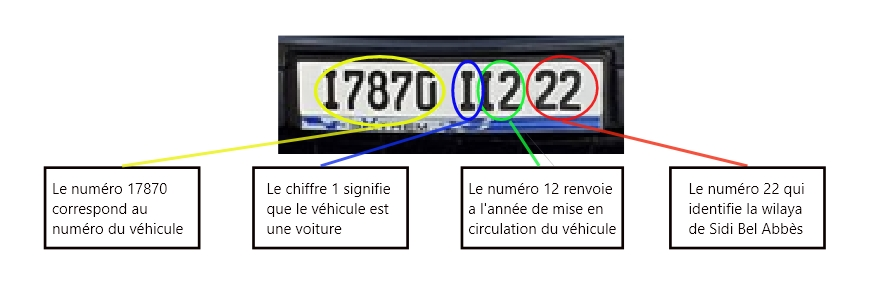
\includegraphics[height=5cm]{ch3-immatriculation.jpg}
	\caption{ Système d’immatriculation des véhicules Algériens}
\end{figure}

%Toutes les plaques d’immatriculation Algériennes \cite{akacem2015reconnaissance} respectent les mêmes caractéristiques, comme illustré dans le tableau \ref{tab:plaques}.

%\begin{table}[h]
%\centering
%\small
%\begin{tabular}{|c|c|c|c|c|c|}
%\hline
%Critères & Épaisseur (mm) & Largeur (cm) & Longueur (cm) & Métal de fabrication & Couleur \\
%\hline
%Plaques d'immatriculation & 1 & 11 & 52 & Aluminium & Blanc en avant et jaune en arrière. \\
%\hline
%\end{tabular}
%\caption{Caractéristiques des plaques d'immatriculation}
%\label{tab:plaques}
%\end{table}


\begin{table}[h]
\centering
%\small
%\footnotesize
\scriptsize
\begin{tabular}{|c|c|c|c|c|}
\hline
  Épaisseur (mm) & Largeur (cm) & Longueur (cm) & Métal de fabrication & Couleur des chiffres\\
\hline
 1 & 11 & 52 & Aluminium & \begin{tabular}[c]{@{}c@{}} Blanc en avant\\ et jaune en arrière\end{tabular} \\
\hline
\end{tabular}
\caption{Caractéristiques des plaques d'immatriculation Algériennes}
\label{tab:plaques}
\end{table}

Aussi, les caractères alphanuériques (ou chiffres arabes) des plaques d'immatriculation doivent être de 7,5 centimètres de haut et doivent être distincts du reste de la plaque de 0,5 millimètre, avec une couleur noire. 
 

\section{Travaux connexes}

De nombreux chercheurs ont consacré leurs efforts à résoudre les défis liés à la détection des véhicules, à l'identification des plaques d'immatriculation, au suivi des véhicules, ainsi qu'à la reconnaissance des caractères alphanumériques figurant sur les plaques d'immatriculation en utilisant les avancées de la vision par ordinateur. 

Dans le cadre de notre projet, nous nous concentrons spécifiquement sur l'étude des plaques d'immatriculation algériennes, car notre objectif principal concerne la gestion des parkings en Algérie.\\
Dans cette revue littéraire, nous passons en revue les travaux les plus récents (2019-2023) que nous avons considérés comme pertinents pour notre domaine de recherche en incluant les travaux portant sur les problématiques suivantes:\\
- La détection des véhicules algériens.\\
- La détection des plaques d’immatriculation algériennes.\\
- La reconnaissance des chiffres présents sur les plaques d'immatriculation .\\
- Le suivi des véhicules.

Boukemoum (2019) \cite{boukemoum-master} a présenté une approche visant à classifier les véhicules algériens et à détecter ceux en mouvement. L'approche comprend les étapes suivantes: 1) Acquisition de deux bases de données , à savoir des vidéos et des images à l'aide d'une caméra, 2) Prétraitement des images acquises en utilisant un filtre médian, 3) Détection des véhicules en mouvement en calculant la différence entre l'image courante et l'image de fond, 4) Une fois les objets en mouvement identifiés dans la scène, l'extraction des caractéristiques est réalisée en utilisant l'histogramme de gradients orientés (HOG), et 5) Classification d'images au moyen d'un modèle SVM.
L'auteur a créé deux bases de données pour cette étude. La première base de données comprend 100 images réparties en deux classes, tandis que la deuxième contient uniquement 3 vidéos. Le modèle SVM a atteint un taux de classification correcte de 84\%, avec une erreur moyenne de classification de 50\% (avec un taux de faux positifs de 79\% et un taux de faux négatifs de 21\%).
 


Abdouche et Allouche (2021) \cite{abdouche-memoire} ont proposé un système visant à classifier, suivre et compter les véhicules en mouvement. L'approche commence par redimensionner les images (frames) utilisées, puis elle utilise un modèle CNN pour apprendre et classifier les images de test en tant que véhicules ou non véhicules. Enfin, le comptage des véhicules est réalisé en combinant plusieurs étapes, notamment le seuillage, la dilatation des résultats segmentés, et le suivi des véhicules en mouvement basé sur les centroïdes des véhicules segmentés. Pour évaluer leur système, les auteurs ont utilisé un jeu de données composé de quatre séquences vidéo distinctes. Les résultats montrent une précision de comptage globale d'environ 90\%. Plus précisément, le système a obtenu une précision de 97,77\% sur la séquence "Route", 97,91\% sur la séquence "Alger", 97,02\% sur la séquence "London", et 95,65\% sur la séquence "Carvidéo".


Guendouz (2020) \cite{guendouz-master} a employé un MLP pour effectuer la reconnaissance des plaques d'immatriculation. L'idée est comme suit: 1) Collecte de données, comprenant des images et des vidéos. 2) Prétraitement des données, impliquant une amélioration du contraste. 3) Opération de détection de contours basée sur le filtre de Sobel. 4) Extraction des caractéristiques en utilisant le détecteur de Harris. (5) Segmentation de l'objet d'intérêt, en l'occurrence les chiffres présents dans les plaques. 6) Classification des images des chiffres par un MLP.\\
En ce qui concerne la base de données, l'auteur a utilisé un ensemble de données contenant 2000 images contenant les chiffres des plaques d'immatriculation. L'approche proposée a obtenu une précision de 98,8\%.

Gadoui et Kebir (2020) \cite{gadoui-kebir-master} ont mis en place un système de détection et de reconnaissance des plaques d'immatriculation des véhicules algériens. Le système effectue ces deux tâches de la manière suivante : 1) Il normalise d'abord les images utilisées, puis les convertit en images en niveaux de gris pour la segmentation. 2) Un filtre Prewitt est appliqué pour détecter les contours des véhicules. 3) Des opérations morphologiques sont utilisées pour améliorer la qualité de la segmentation des plaques d'immatriculation. 4) Ensuite, une projection verticale et horizontale de l'image est effectuée pour localiser la plaque d'immatriculation dans l'image. 5) En se basant sur les caractéristiques de la projection verticale des caractères en binaire et sur l'extraction des composants connexes, les auteurs parviennent à localiser les plaques d'immatriculation. 6) Pour la reconnaissance des chiffres présents sur la plaque, la technique de la matrice de distribution est utilisée avec un classifieur SVM. Le système parvient à atteindre un taux de reconnaissance des chiffres de 98,74\% sur un ensemble de 36 plaques d'immatriculation. 

% Ajouter refBen : An ALPR System-based Deep Networks for the Detection and Recognition
% ajouter la réference au tableaux : résumé des travaux connexes

Bensouilah et al. (2021) \cite{bens} ont présenté une nouvelle base de données ainsi qu'un système robuste de reconnaissance des plaques d'immatriculation algériennes, en utilisant le détecteur d'objets YOLOV3. Ensuite, un CNN est employé pour extraire les caractéristiques des plaques d'immatriculation, suivi d'un RNN pour la reconnaissance des caractères présents sur les plaques. Les résultats des expériences étaient concluants, avec un taux de reconnaissance de 92\% sur un ensemble d'images de 2408.

Hammoudi et Kechra (2022) \cite{hammoudi-kechra-master} ont élaboré un système automatisé de détection et de reconnaissance des véhicules. Le concept sous-jacent de ce système peut être décrit comme suit : Tout d'abord, les images sont dimensionnées et converties en images en niveaux de gris. Ensuite, un filtre bilatéral est appliqué à ces images pour éliminer les détails indésirables. La prochaine étape implique l'application du filtre de Canny pour détecter les contours des objets. Une fois que les contours sont détectés, les résultats de la détection sont triés et filtrés afin de sélectionner la région d'intérêt, qui contient les chiffres de la plaque d'immatriculation.
La phase suivante de la reconnaissance de la plaque d'immatriculation implique la segmentation et la localisation des chiffres présents dans la plaque.
Enfin, la dernière étape consiste à reconnaître les chiffres de la plaque à partir de l'image segmentée en utilisant le package Cascade.
Les résultats expérimentaux démontrent un précision de reconnaissance de 85\%  sur un ensemble de 70 images de véhicules.

 % Ajouter refZiban : A New Fusion-Based Approach for License Plate Recognition: An Application to the Algerian Context
% Ajouter cette référence dans le tableau: résumé des travaux connexes

Zibani et al. (2022) \cite{zibani} ont proposé une nouvelle approche de reconnaissance de plaques d'immatriculation basée sur la fusion de données. Cette approche comprend deux étapes principales : 1) Segmentation des plaques d'immatriculation en utilisant deux méthodes différentes, à savoir le YOLO object finder (YOLO) et la détection de contours. 2) Classification des caractères présents sur les plaques segmentées en utilisant plusieurs classifieurs tels que le SVM, le CNN et le LSTM. Ces classifieurs sont ensuite combinés à l'aide de techniques de fusion de données, notamment la théorie de l'évidence et la méthode de vote majoritaire. Les auteurs ont constitué une base de données de 1000 images de plaques d'immatriculation algériennes pour évaluer leur approche. Les résultats obtenus montrent que le taux de reconnaissance moyen est de 98,7 \%.


Le tableau \ref{tab:research-summary} résume l'ensemble des travaux que nous avons identifiés dans la littérature.

\begin{table}[h]
\centering
\scriptsize
\begin{tabular}{|p{1.5cm}|c|p{3cm}|p{2.5cm}|c|p{1cm}|p{1cm}|}
%{|p{1.5cm}|c|p{1.5cm}|p{2cm}|c|p{1cm}|p{1cm}|}
\hline
Auteur & Date & Objectif & Jeu  de données & Modèle & Métrique \\
\hline
Boukemoum & 2019 & Détection des véhicules  & Collecte manuelle des données (130 images
3 vidéos) & HOG, SVM & 94.44\% \\

\hline
Abdouche  et Allouche  & 2019 & Détection et comptage des véhicules en mouvement & 4 séquences vidéo  & CNN combiné avec une   & 97\% \\
& & & & approche de comptage basée & \\
& & & & sur les centroid des plaques détectées & \\
\hline
Gundouz & 2019 & Reconnaissance automatique des plaques d’immatriculation algériennes & 2000 images rassemblées sur Internet & MLP & 98,8\% \\
\hline
Gadoui et Kebir & 2019 & Lecture automatique de plaques d'immatriculation & 400 images collectés sur internet & SVM & 98.74\% \\

\hline
Bensouilah et al. & 2021  &  Reconnaissance des plaques d'immatriculation  &  2408 images & YOLOv3, CNN et RNN &  92\%\\

\hline
Hammoudi et Kechra  & 2022 & Identification automatique des véhicules & 70 images collectées sur internet & Combinaison des approches:  & 85\% \\
& & & & détection des contours,  & \\
& & & & segmentation et framework cascade & \\

\hline
Zibani et al. & 2022 & Reconnaissance des plaques d'immatriculation & 1000 images & YOLO Object Finder, & 98,7\% \\
& & & & détection de contours  & \\
& & & &  SVM, CNN, LSTM & \\

\hline

% Ajouter cette ligne
%\hline
% Zibani et al.   &  2022  & Reconnaissance des plaques d'immatriculation   &  1000 images  & Ensemble des méthodes (YOLO object Finder, détection de contours, SVM, CNN et LSTM)   &  98,7\% \\

\end{tabular}
\caption{Résumé des travaux connexes}
\label{tab:research-summary}
\end{table}


\section{Synthèse des travaux connexes}

D'après l'étude réalisée, plusieurs approches ont recours au classifieur SVM ou à des réseaux de neurones profonds pour la détection des véhicules, des plaques d'immatriculation, et la reconnaissance des chiffres présents sur les plaques.

Un autre aspect qui a retenu notre attention est la complexité des approches proposées, en particulier celles qui font usage de modèles d'apprentissage classiques. En général, ces modèles ont recours au prétraitement des données manipulées en raison de la qualité des images traitées.

En outre, il est important de noter que la plupart des travaux reposent sur des bases de données de taille réduite, ce qui limite les performances de la détection et/ou de la reconnaissance.

Dans le cadre de notre projet, nous cherchons à développer un système de gestion de parking relativement basique, tout en visant à améliorer les résultats en utilisant des techniques avancées, notamment en nous appuyant sur le détecteur YOLOv8. Il serait également essentiel que le système de gestion de parking que nous souhaitons développer puisse détecter les véhicules, les plaques d'immatriculation, reconnaître les chiffres d'immatriculation et suivre les véhicules en temps réel pour répondre efficacement aux besoins de gestion de parking.



\section{Jeux de données disponibles}

Généralement, les algorithmes de détection et de reconnaissance à base d'apprentissage automatique nécessitent un ensemble de données avec une quantité substantielle de données diverses, équilibrées et de hautes qualités pour obtenir de meilleur résultat. 

Nous citons ci-dessous les jeux de données algériens disponibles pour la détection des véhicules, des plaques d'immatriculation et la reconnaissance des chiffres alphanumériques

\begin{itemize}
    \item [$\bullet$] Le jeu de données "ALP" \cite{license-dataset} est un ensemble de données (images et vidéos) de plaques d'immatriculation algériennes capturées dans la municipalité de Draria en Algérie à l'aide d'une caméra fixe. 
    Il a également été enrichi par les auteurs de l'article \cite{bens} avec des images provenant de sites tels que "Google Images", "Facebook Marketplace" et "Ouedkniss". Ce jeu de données comprend 1000 images de plaques d'immatriculation algériennes, couvrant une variété de poses, de conditions d'éclairage et d'occlusions.   
    %%%Ajouter ref1: https://github.com/mouadb0101/License_Plates_of_Algeria_Dataset}
    %%%Ajouter ref2: An ALPR System-based Deep Networks for the Detection and Recognition
    \item [$\bullet$] Le jeu de données "Algerian Vehicle Dataset" est un ensemble de données de véhicules algériens collecté par les auteurs de l'article \cite{zibani}. Le jeu de données contient 1000 images de véhicules algériens, avec une variété de poses, de conditions d'éclairage et d'occlusions.
     %%%Ajouter ref3: A New Fusion-Based Approach for License Plate Recognition: An Application to the Algerian Context
\end{itemize}
En plus de ces ensembles de données, il existe également plusieurs ressources en ligne qui peuvent être utilisées pour collecter des images de plaques d'immatriculation algériennes. Par exemple, le site web Ouedkniss permet aux utilisateurs de vendre et d'acheter des voitures d'occasion en Algérie. Les images de voitures sur ce site web peuvent être utilisées pour collecter des images de plaques d'immatriculation algériennes.

Nous constatons en effet que le nombre de jeux de données disponibles est limité. Ces ensembles de données ont généralement un nombre restreint d'échantillons, ce qui a un impact sur le taux de reconnaissance et/ou de détection, en particulier dans les approches d'apprentissage profond. De plus, les ensembles de données enregistrés sont souvent conçus pour un objectif spécifique de détection ou de reconnaissance, ce qui limite leur polyvalence et leur utilisation dans des contextes différents.

\section{Frameworks utilisés en apprentissage profond}

Il existe plusieurs frameworks d'apprentissage profond populaires qui sont largement utilisés par la communauté de l'apprentissage automatique. Voici quelques-uns des cadres les plus populaires :
\begin{itemize}
    \item [$\bullet$] Tensorflow: est un framework open source d'apprentissage automatique développé par Google. Il est utilisé pour créer, former et déployer des modèles d'apprentissage automatique, en particulier des réseaux de neurones profonds. TensorFlow offre un calcul numérique flexible, la gestion automatique des gradients, et prend en charge diverses architectures de réseaux de neurones. Il bénéficie d'une large communauté, est flexible pour le déploiement, prend en charge le calcul parallèle, et peut être intégré avec d'autres bibliothèques telles que Keras. Il est largement utilisé dans de nombreuses applications d'intelligence artificielle et de vision par ordinateur\cite{ch3_TensorFlow}.
    \item [$\bullet$] Keras :Keras est une bibliothèque d'apprentissage automatique open-source très accessible et conviviale, conçue pour développer des modèles de réseaux de neurones. Il permet aux développeurs de créer, former et évaluer facilement différents types de modèles d'apprentissage profond. Keras est couramment utilisé dans la recherche en apprentissage profond et le développement d'applications d'intelligence artificielle en raison de son interface simple et cohérente. Depuis TensorFlow 2.0, Keras est intégré à TensorFlow en tant que "tf.keras", ce qui facilite son utilisation avec TensorFlow \cite{ch3_KerasDee40}.
     \item [$\bullet$] OpenDeep : est un framework d'apprentissage profond pour Python, destinée à un usage commercial et de recherche. Il est construit à partir de Theano et est entièrement modulaire et facilement extensible. OpenDeep est conçue pour être flexible et facile à utiliser pour les scientifiques de données de l'industrie et les chercheurs universitaires. Il permet de construire n'importe quelle architecture de réseau de neurones pour résoudre des problèmes d'apprentissage profond \cite{ch3_opendeep}. 
    \item [$\bullet$] PyTorch: est un framework open-source d'apprentissage automatique développé par Facebook. Il offre une interface Python conviviale pour la création de modèles d'apprentissage automatique flexibles \cite{datascientest-pytorch}. L'une de ses caractéristiques distinctives est son système de calcul de gradient automatique (Autograd), qui permet de calculer automatiquement les gradients des fonctions définies par l'utilisateur, simplifiant ainsi la création de modèles complexes. Les poids des modèles dans PyTorch sont généralement enregistrés avec les extensions ".pt" ou ".pth" dans des fichiers au format TorchScript, facilitant la réutilisation des modèles entraînés sur de nouvelles données ou leur déploiement en production.
    \item [$\bullet$] NCNN est un framework de calcul d'inférence de réseau neuronal hautes performances optimisé pour les plates-formes mobiles et sur des dispositifs à ressources limitées, tels que des smartphones, des appareils embarqués et des microcontrôleurs. Il se distingue par sa haute performance et sa faible consommation de mémoire, ce qui le rend adapté aux applications de traitement d'image en temps réel. NCNN prend en charge diverses plates-formes matérielles, notamment les processeurs ARM, les GPU. Un aspect remarquable de NCNN est sa compatibilité avec différentes plates-formes matérielles, lui permettant de tirer parti de l'accélération matérielle pour des performances accrues en apprentissage automatique. NCNN propose un large éventail d'opérations de réseaux neuronaux, comme la convolution, la normalisation, et le regroupement (pooling). De plus, il offre des outils de conversion de modèles à partir d'autres cadres d'apprentissage automatique, comme PyTorch et TensorFlow, vers son propre format de modèle optimisé pour des performances maximales. Les fichiers de poids dans NCNN ont généralement l'extension ".param" et ".bin" et stockent respectivement l'architecture du modèle et les paramètres appris. Ils sont utilisés pour charger des modèles pré-entraînés et effectuer des inférences. NCNN est largement utilisé dans diverses applications de Tencent \cite{ch2_GitHubTe84}, telles que QQ, Qzone, WeChat et Pitu.
\end{itemize}

 \section{Conclusion}

Cette étape de recherche scientifique a été cruciale pour ce projet. Au cours de ce chapitre, nous avons pu identifier les travaux les plus récents liés à la gestion du stationnement des véhicules en Algérie, réalisés en utilisant des modèles d'apprentissage automatique (classiques et profonds). Cette recherche scientifique nous a également permis de proposer une solution potentielle qui pourrait être développée en suivant des étapes clairement définies.

\chapter{Système intelligent de gestion du parking: Réalisation, résultats et analyse}
\markboth{Système intelligent de gestion du parking: Réalisation, résultats et analyse}{}
\section{Introduction}
% ------------------------------------------ ok
% Ajouter les 3 rférences de OCR  EASYOCR,...
Les trois premiers chapitres offrent un aperçu de la gestion des parkings et explorent les diverses solutions envisageables grâce à l’intégration de l'intelligence artificielle. 

ce dernier chapitre se concentre spécifiquement sur notre système de gestion de parking intelligent, qui est construit sur la base du modèle YOLOv8. Ce système a la capacité de détecter les véhicules, de reconnaître les plaques d'immatriculation, d'identifier les caractères optiques présents sur ces plaques, de suivre en temps réel les mouvements des véhicules dans le parking, et de calculer le nombre de véhicules entrants et sortants. 
Dans le cadre du développement de ce système, nous avons évalué plusieurs modèles, notamment EasyOCR\cite{ch4_EasyOCRV83}, OpenALPR\cite{ch4_OpenALPR81} et Tesseract-ocr\cite{tesseract-ocr-guide}, FASTER\_RCNN\_MOBILENET, SSDLITE\_MOBILENET, et avons obtenu des résultats diversifiés. Compte tenu du manque de bases de données spécialisées, nous avons créé notre propre base de données contenant des informations sur les véhicules en Algérie pour évaluer notre système. Enfin, nous présentons les défis auxquels nous avons été confrontés lors de la mise en œuvre du système et analysons les résultats que nous avons obtenus.

\section{Problématique et motivation}

Avec les progrès constants dans l'industrie du stationnement, l'intégration de technologies de reconnaissance, telles que la détection des voitures, la détection des plaques d'immatriculation, la reconnaissance des caractères optiques et le suivi des mouvements des véhicules, s'avère cruciale pour améliorer l'expérience des conducteurs et optimiser l'utilisation de l'espace de stationnement. En identifiant des éléments spécifiques, tels que les voitures et les plaques d'immatriculation, à partir de l'ensemble des données recueillies, le système peut exécuter des actions précises, comme l'attribution d'un emplacement de stationnement ou la gestion des paiements.

Par conséquent, l'utilisation d'algorithmes d’intelligence artificielle sera nécessaire pour reconnaître ces éléments et prendre des décisions en temps réel. Actuellement, l'apprentissage en profondeur a été largement appliqué avec succès (obtenant des performances exceptionnelles) pour résoudre différents problèmes liés à la vision par ordinateur, notamment dans le domaine de la détection d'objets et de la reconnaissance optique de caractères. Étant donné que les applications de gestion de parking intelligent sont également des systèmes en temps réel avec des contraintes temporelles spécifiques, l'utilisation de modèles de détection d'objets en temps réel, tels que YOLOv8, peut être pertinente pour obtenir des résultats rapides et précis.\\
En outre, il pourrait être avantageux de disposer de bases de données spécifiques à l’Algérie pour tester notre système de gestion de parking intelligent. Cela permettrait de garantir une solution plus adaptée, conforme et efficace pour répondre aux besoins spécifiques du contexte de gestion de parking en Algérie.

\section{Solution proposée}
La solution proposée repose sur trois sous-systèmes , qui sont inter-connectés pour former un système global de gestion de parking intelligent, comme illustré dans la figure \ref{fig:ch4_Simple_system_diagram}. 

\begin{outline}
    \1 Le premier sous-système est utilisé pour détecter les voitures et les plaques d'immatriculation dans une image.

    \1 Le deuxième sous-système se focalise sur la reconnaissance des caractères optiques contenus sur la plaque détectée. 

    \1 Le troisième  sous-système  suit les mouvements des voitures dans une vidéo en temps réel.
\end{outline}

\begin{figure}[H]
	\centering
	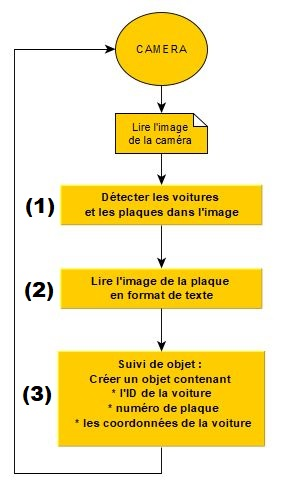
\includegraphics[height=05cm]{ch4-Simple_system_diagram.jpg}
	\caption{Système proposé de gestion de parking intelligent}
 \label{fig:ch4_Simple_system_diagram}
\end{figure}
\subsection{Sous-systèmes de détection de véhicules et de plaques d'immatriculations}
Comme mentionné précédemment, ce travail s'appuie sur le modèle "YOLOv8", "SSD" ou "Faster R-CNN" pour la gestion des parkings. Ce processus implique l'identification et la prédiction des véhicules ainsi que des plaques d'immatriculation Algériennes, réparties en deux catégories : véhicules et plaques d’immatriculation.
\\
L'idée est de construire d'abord une base de données de véhicules, puis d'entraîner le modèle et de le tester sur des images. Pour ce faire, les images collectées sont soumises à un prétraitement et à une annotation. Ensuite, un échantillonnage automatique des données est appliqué pour former des ensembles d'images destinés à l'entraînement, à la validation et aux tests.
%(70 \%) des images de données ont été utilisées comme échantillons d'apprentissage.
%(20 \%) des images de données ont été utilisées comme ensembles de validation.
%(10\%) des images de données ont été utilisées comme ensembles de test.

Dans la phase d'apprentissage du modèle adapté, les poids du modèle sont calculés en se basant sur les ensembles de données préparés et les poids pré-entraînés. Une fois que l'apprentissage est terminé, il est nécessaire d'évaluer le modèle utilisé sur des données de test en utilisant les poids d'entraînement. Par conséquent, les véhicules munis de plaques d'immatriculation à détecter seront localisés et prédits.


Après cela, l'algorithme et le modèle appropriés sont sélectionnés pour effectuer la tâche de détection de la voiture et de la plaque d'immatriculation sur la base des résultats obtenus.

\subsection{ Sous-système destiné à la reconnaissance des numéros de la plaque d'immatriculation}\label{sec:ocr_by_object_detection}

Après la détection de la voiture et de la plaque d'immatriculation dans l'image, le système extrait la zone correspondante de la plaque d'immatriculation de l'image détectée. Cette zone est utilisée pour créer une nouvelle image. Ensuite, le modèle de détection formé sur les numéros de plaque d'immatriculation entre en jeu pour reconnaître les caractères alphanumériques en utilisant les mêmes étapes que dans le système de détection de voiture et de plaque d'immatriculation, à savoir l'échantillonnage, la formation, le test et la vérification de la validité.

La liste des numéros détectés est ensuite organisée dans l'ordre de leur position dans l'image, de gauche à droite, afin de former une chaîne de caractères avec ces numéros, comme illustré dans la figure \ref{fig:ch4-Ocr_my_001}.
\begin{figure}[H]
	\centering
	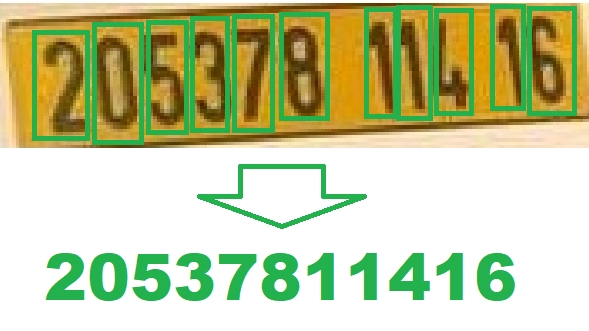
\includegraphics[height=05cm]{ch4-Ocr_my_001.jpg}
	\caption{ Reconnaissance des numéros de la plaque d'immatriculation}
    \label{fig:ch4-Ocr_my_001}
\end{figure}

\subsection{Sous-systèmes de suivi et de comptage en temps réel des véhicules}\label{sec:traking}


Les véhicules identifiés sont exploités dans le processus de suivi et de comptage des véhicules au sein d'une séquence vidéo. Cette séquence enregistre des images de véhicules capturées à des moments successifs. Par conséquent, lorsqu'un véhicule est observé en mouvement dans une vidéo, cela implique que le véhicule occupe une position différente à chaque image consécutive de la vidéo.
\\
L'idée fondamentale derrière le suivi d'objets réside dans la création d'un traqueur d'objet pour chaque objet détecté, afin de suivre son déplacement. Ce suivi se prolonge jusqu'à ce que la N-ième image de la séquence soit atteinte, avec un processus de détection d'objets en cours. Le traqueur d'objets est responsable de la surveillance continue de chaque véhicule, attribuant et maintenant des numéros d'identification (ID) pour chacun.

Dans la phase de suivi de notre système, nous avons mis en œuvre un algorithme simple de suivi d'objets qui se base sur le suivi des centroïdes des objets. Il fonctionne en calculant la distance Euclidienne entre les centroïdes des véhicules déjà existants (c'est-à-dire les véhicules précédemment suivis par le traqueur de centroïdes) et les centroïdes des nouveaux véhicules présents dans les images suivantes de la vidéo. Les étapes complètes de cette solution sont détaillées comme suit :

%Ces étapes sont répétées tout le temps tant que le programme est en cours d'exécution 
\begin{outline}[enumerate]
    \1  Lire un image de la vidéo (ou d'un flux de données en temps réel)à un moment t.
    
    \1  Détecter les véhicules présents dans l'image (en estimant les coordonnées des boîtes englobantes) concernée.
    
    \1  Attribuer un identifiant à chaque véhicule détecté.
    
    \1  Calculer les centroïdes des voitures détectées et les enregistrer dans une liste. 
    
    \1  Lire un nouvelle image de la vidéo à un moment t+1.
    
    \1  Détecter les véhicules présents dans la nouvelle image (en estimant les coordonnées des nouvelles boîtes englobantes).
    
    \1  Calculer la distance entre les centroïdes des nouveaux véhicules et tous les centroïdes d'objets enregistrés dans la liste précédente.Si la distance entre le centre du nouveau véhicule et l'un des centres de la liste est inférieure à une distance minimale prédéfinie, alors le véhicule détecté est considéré comme étant le même que celui déjà enregistré. Le centroïde nouvellement calculé remplace l'ancien centroïde, et l'identifiant reste inchangé. Si la distance entre le centroïde du nouveau véhicule et tous les centres enregistrés dans la liste précédente est supérieure à la distance minimale, alors ce véhicule est considéré comme un nouveau véhicule dans la vidéo. Son centroïde est ajouté à la liste des centroïde avec un nouvel identifiant.
\end{outline}

Si nous divisons la scène sous surveillance de la caméra de sécurité en deux zones,  à savoir la zone B près de la porte du parking et la zone A plus éloignée de la porte du parking, comme illustré dans la figure \ref{ch4-comptage}, il devient possible de compter les véhicules entrants et sortants en suivant le mouvement des véhicules entre les deux zones de la manière suivante :\\
Lorsque nous suivons les véhicules qui se déplacent de la zone A vers la zone B, nous les comptons et les considérons comme le nombre de véhicules entrant dans le parking.\\
Lorsque nous suivons les véhicules qui se déplacent de la zone B vers la zone A, nous les comptons et les considérons comme le nombre de véhicules sortant du parking.

\begin{figure}[H]
	\centering
	\includegraphics[height=05cm]{ch4-comptage.jpg}
	\caption{ Comptage des véhicules}
    \label{ch4-comptage}
\end{figure}

\section{Étude expérimentale}

Les expériences réalisées dans cette section ont été effectuées en utilisant le langage de programmation Python sur la plateforme Google Colaboratory (communément appelée Colab). Cette plateforme utilise l'environnement "Jupyter" (exécuté dans le cloud de Google) pour des tâches d'apprentissage profond et des applications centrées sur les unités de traitement graphique (GPU). En plus de sa facilité d'utilisation (aucune installation préalable requise), Colab offre des ressources de calcul gratuites et prend en charge le développement collaboratif. Du point de vue technique, elle est équipée de 12,8 Go de mémoire vive (RAM) et d'une unité de traitement graphique gratuite (NVIDIA Tesla t4 + 16GB RAM) pouvant être utilisée en continu pendant 12 heures, avec la possibilité d'accéder à d'autres unités de traitement moyennant un abonnement payant. En complément, nous avons utilisé un ordinateur portable équipé d'un processeur \{Intel i5-8350U à 1,70 GHz\}, avec une carte graphique \{Intel UHD Graphics 620\}, sous Windows 10  pour réaliser nos expériences.
Le framework Pytorch est également employé pour construire notre modèle d'apprentissage profond pour la gestion de parking. 

\subsection{Description des jeux de données}

L'initiation du processus de gestion de parking implique la collecte de données d'images. Toutefois, il est ardu de trouver un ensemble de données spécialement conçu pour détecter les véhicules avec des plaques d'immatriculation Algériennes. De surcroît, cet ensemble d'images doit être suffisamment vaste, préserver les détails et bénéficier d'une qualité élevée. En réalité, un tel ensemble de données n'est pas encore disponible.

Dans le cadre de ce travail, nous élaborons notre propre ensemble de données ce qui garantit que les algorithmes de détection ainsi que la reconnaissance peuvent gérer les scénarios et les contextes typiques de l'environnement de gestion de parking de véhicules Algériens.
Dans la section actuelle, nous décrivons le processus de préparation des jeux de données générés, qui visent à: 

\begin{itemize}
\item (1) Détecter les véhicules et les plaques d'immatriculation.
\item (2) Reconnaître les caractères optiques.
\end{itemize}

% ++++++++++++++++++++++++++++++++++++++++++++++++++++++++++++++++++++++++++++++++++++++++++ car

\subsubsection {(1) Jeu de données destiné pour la détection des véhicules et des plaques d'immatriculation Algériennes}


% ++++++++++++++++++++++++++++++++++++++++++++++++++++++++++++++++++++++++++++++++++++++++++ car Collecte d'images

\textbf{Collecte d'images}

Les images ont été rassemblées à partir de deux sources principales :
\begin{itemize}
    \item [$\bullet$] Ouedkniss : un site spécialisé dans la vente d'articles neufs et d'occasion. Ce site abonde en photos de voitures Algériennes proposées à la vente. Pour ce faire, nous avons développé un script Python qui explore le site Ouedkniss, détecte les annonces de voitures et enregistre automatiquement les images dans un fichier.
    
    \item [$\bullet$] Facebook : une plateforme de médias sociaux offrant divers services. Parmi ces services, nous avons exploité la possibilité de collecter un grand nombre de photos de voitures mises en vente. Le téléchargement de ces photos a été effectué manuellement.
    
\end{itemize}
Au total, près de 5000 images ont été collectées à partir de ces deux sources.

% ++++++++++++++++++++++++++++++++++++++++++++++++++++++++++++++++++++++++++++++++++++++++++ car Pré-traitement

\textbf{Pré-traitement des images}

Étant donné que l'ensemble de données que nous avons collecté contient de nombreuses images de mauvaise qualité, nous avons exclu 2620 de ces images. En conséquence, le nombre final d'images est passé à 2380.

% ++++++++++++++++++++++++++++++++++++++++++++++++++++++++++++++++++++++++++++++++++++++++++ car Annotation

\textbf{Annotation des données}

L'annotation manuelle est une tâche extrêmement exigeante, c'est pourquoi il est souvent préférable d'utiliser des outils qui simplifient le processus. Plusieurs options sont disponibles parmi ces outils, dont Roboflow et labelme. Cependant, après une utilisation prolongée de ces deux outils, nous avons rencontré plusieurs problèmes :
\begin{outline}
    \1  Annotation par Roboflow : bien qu'il s'agisse d'un site web, son utilisation a ralenti considérablement le processus d'annotation, en particulier lorsque nous avions un grand nombre d'images à annoter.
    \1 Annotation par labelme : c'est un outil qui s'installe via la ligne de commande Python, mais il a présenté de nombreuses erreurs de programmation. Même après avoir résolu ces erreurs, divers problèmes sont apparus de manière sporadique.
\end{outline}

Nous avons développé notre propre programme qui effectue le processus d'annotation manuel et automatique afin d'affiner les modèles de détection d'objets dans les images. Une fois le développement achevé, nous avons créé une interface graphique en utilisant la bibliothèque PyQt, comme le montre la figure \ref{fig:ch4-yolo_labling_car}.

\begin{figure}[H]
	\centering
	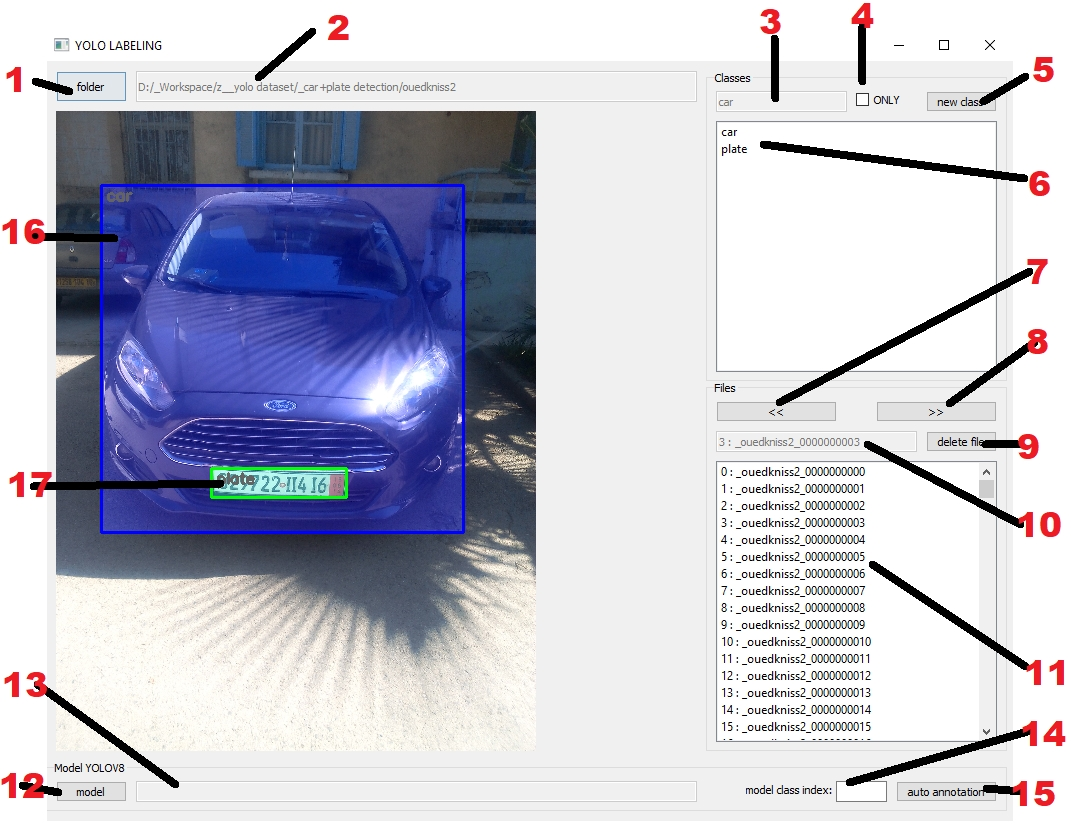
\includegraphics[height=12cm]{ch4-Yolov8_labling.jpg}
	\caption{Annotation des images}
 \label{fig:ch4-yolo_labling_car}
\end{figure}

Sachant que:
\begin{outline}

    \1 1 :  Ce bouton permet de choisir le dossier de travail contenant les images que nous souhaitons utiliser pour générer des étiquettes ("voiture" et "plaque d'immatriculation") et former un modèle de détection d'objet.
    
    \1 2 : Le chemin du dossier de travail actuellement sélectionné s'affiche ici.
    
    \1 3 : Nous pouvons sélectionner la classe d'objet à annoter dans les images. 
    
    
    \1 4 : En sélectionnant un objet dans une image donnée, seuls la boite de délimitation correspondant à cette classe seront affichés.
    
    
    \1 5 : Utiliser ce bouton pour créer une nouvelle classe.
    
    \1 6 : Cette liste affiche toutes les classes disponibles dans la base de données.
    
    \1 7 : Ce bouton nous permet de revenir à l'image précédente.
    
    \1 8 : Bouton pour passer à l'image suivante.
    
    \1 9 : Nous pouvons effacer le fichier image actuel et les annotations associées en utilisant ce bouton.
    
    \1 10 : Le chemin de l'image sur laquelle nous travaillons est affiché ici.
    
    \1 11 : Cette liste présente toutes les images présentes dans le dossier de travail.
    
    
    \1 12 : Sélection d'un modèle de détection d'objets pré-entraîné, tel que YOLOv8, pour générer automatiquement des légendes pour les images.
    
    \1 13 : Le chemin du modèle de détection d'objets YOLOv8 pré-entraîné est indiqué ici.
    
    \1 14 : Entrer le numéro de classe que nous souhaitons que le programme détecte dans les images du dossier de travail. Une fois que ses coordonnées sont identifiées dans les images, le programme génère des annotation pour la classe sélectionnée et enregistre.
    
    \1 15 : Ce bouton démarre le processus de génération automatique des étiquettes pour les images. 

\end{outline}
A la fin, le fichier d'annotation sera créé automatiquement avec le même nom que l'image avec une extension txt.

% ++++++++++++++++++++++++++++++++++++++++++++++++++++++++++++++++++++++++++++++++++++++++++ car Échantillonnage

\textbf{Échantillonnage de données}
\par Dans l'échantillonnage de données, nous avons divisé notre premier jeu de données en trois ensembles distincts : un ensemble d'entraînement, un ensemble de validation et un ensemble de test, en respectant les proportions suivantes :

\begin{outline}

\1 70\% (1667 images) de l'ensemble de données est utilisé pour l'entraînement (Training set).

\1 20\% (475 images) de l'ensemble de données est réservé à la validation (Validation set).

\1 10\% (238 images) de l'ensemble de données est dédié aux tests (Testing set).

\end{outline}

Cette approche est courante dans le domaine de l'apprentissage automatique, où le partitionnement se fait comme le montre la figure \ref{fig:split_dataset_car}.

\begin{figure}[H]
	\centering
	\includegraphics[height=02cm]{ch4-split01.jpg}
	\caption{Échantillonnage du jeu de données}
    \label{fig:split_dataset_car}
\end{figure}

% ++++++++++++++++++++++++++++++++++++++++++++++++++++++++++++++++++++++++++++++++++++++++++ car Augmentation 

\textbf{Augmentation du jeu de données}

L'augmentation de données est une technique couramment utilisée dans le domaine de l'apprentissage automatique pour améliorer les performances des modèles prédictifs en fournissant l'avantage de variations de données d'entraînement disponibles. L'idée principale derrière l'augmentation de données est de générer de nouvelles données (d'apprentissage) en appliquant des transformations ou des manipulations aux données (d'apprentissage) d'origine, tout en préservant leur sémantique et leur classe.
Les avantages de l'augmentation de données comprennent :

\begin{outline}
\1 Elle augmente la taille de données d'entraînement disponibles, en réduisant ainsi le risque de sur-ajustement (overfitting) et en améliorant la capacité du modèle à reconnaître de nouveaux motifs et caractéristiques plus robustes.
\1 Elle aide à renforcer la capacité du modèle à traiter les variations dans les données réelles.
\1 De plus, l'augmentation de données réduit la dépendance à l'égard de vastes quantités de données d'entraînement, ce qui permet de créer des modèles performants avec moins de données.
\end{outline}

Le site Roboflow propose de nombreuses méthodes d'augmentation de données, bien que l'option gratuite offre moins de fonctionnalités et de types d'augmentation de données. Nous avons appliqués sur notre ensemble de données ce qui suit et aussi comme le montre la figure \ref{fig:Augmentation_roboflow}:
\\
- Le retournement horizontal, la rotation dans la plage de -5° à +5°.\\
- La déformation horizontale et verticale.\\
- La conversion partielle en niveaux de gris pour environ 25\% des images.\\
- L'ajustement de la teinte dans l'intervalle de -23° à +23°.\\
- La modification de la saturation entre -25\% et +25\%.\\
- La variation de la luminosité entre -25\% et +25\%.\\
- La modification de l'exposition dans la plage de -25\% à +25\%.\\
- Le flou jusqu'à 1.25 pixel et l'ajout de bruit jusqu'à 1 pixel.\\

\begin{figure}[H]
	\centering
	\includegraphics[height=07cm]{ch4-augmontation.jpg}
	\caption{Méthodes d'augmentation de données}
    \label{fig:Augmentation_roboflow}
\end{figure}

Après avoir réalisé l'augmentation de données sur l'ensemble d'entraînement,  après qu'elles étaient de 1667, elles sont devenues 5001, alors que nous n'avons pas modifié les données testing et de validation , Les résultats étaient les suivants et comme le montre la figure \ref{fig:Aug}.

Après avoir appliqué l'augmentation de données à l'ensemble d'entraînement, qui est passé de 1667 à 5001 images, nous n'avons pas apporté de modifications aux ensembles de données de test et de validation. Les résultats obtenus sont résumés comme suit:\\
- 88 \% (5001 images) des images de données ont été utilisées comme échantillons d'apprentissage.\\ 
- 8 \% (474 image ) des images de données ont été utilisées comme ensembles de validation.\\ 
- 4 \% (238 images ) des images de données ont été utilisées comme ensembles de test.

\begin{figure}[H]
	\centering
	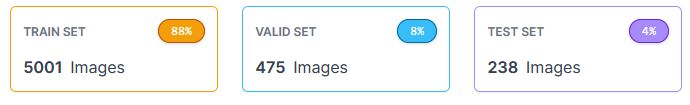
\includegraphics[height=02cm]{img/ch4-Augmentation_car+plate.jpg}
	\caption{Augmentation du jeu de données}
 \label{fig:Aug}
\end{figure}

Une fois que nous avons terminé, nous avons rendu la base de données publique et disponible pour usage en la publiant sur le site web Roboflow à l'adresse suivante : \url{https://universe.roboflow.com/lounisamr/car-plate-dzex/dataset/2}.

%Augmentation du jeu de données


% ++++++++++++++++++++++++++++++++++++++++++++++++++++++++++++++++++++++++++++++++++++++++++ OCR 


\subsubsection {(2) Jeu de données destiné pour la reconnaissance des numéros d'immatriculation }

Pour ce qui est de l'ensemble de données prévu pour la reconnaissance des caractères optiques, nous avons adopté les mêmes étapes que celles utilisées pour l'ensemble de données dédié à la détection des véhicules et des plaques d'immatriculation.

 % ++++++++++++++++++++++++++++++++++++++++++++++++++++++++++++++++++++++++++++++++++++++++++ OCR  Collecte d'images
 
\textbf{Collecte d'images}

Nous avons d'abord développé un script Python qui est capable de lire les images annotées ainsi que leurs fichiers d'annotation associés à partir du premier jeu de données. 
Ensuite, ce script extrait la région qui correspond à la plaque d'immatriculation, la découpe et la sauvegarde en tant que nouvelle image. Le jeu de données ainsi crée comprend un ensemble varié d'images contenant les plaques d'immatriculation Algériennes. L'objectif est de construire un nouveau jeu de données spécifiquement orienté vers la reconnaissance des caractères optiques.

\begin{figure}[H]
	\centering
	\includegraphics[height=07cm]{ch4-crop_plate_001.jpg}
	\caption{Extraction des plaques d'immatriculation.}
    \label{fig:CropPlate}
\end{figure}

 % ++++++++++++++++++++++++++++++++++++++++++++++++++++++++++++++++++++++++++++++++++++++++++ OCR  Pré-traitement
 
\textbf{Pré-traitement des images}

\par Après avoir créé les images de plaques d’immatriculation, nous avons constaté que la majorité de ces images présentaient des problèmes de qualité. Par conséquent, nous effectuons un processus de tri pour ne conserver que les images de la plus haute qualité. C'est pourquoi nous avons développé un script Python qui parcourt toutes les images et supprime celles qui font moins de 200 pixels de large. Ce processus a abouti à un total de 626 images. Ensuite, nous supprimons les photos qui ne répondent pas à nos normes de qualité. A l’issue de cette étape, nous avons pu constituer une collection finale de 417 images de plaques d’immatriculation algériennes de haute qualité.

 % ++++++++++++++++++++++++++++++++++++++++++++++++++++++++++++++++++++++++++++++++++++++++++ OCR  Annotation
 
\textbf{Annotation des numéros d'immatriculation }

\par Pour ajouter des annotations aux caractères sur les images des plaques d'immatriculation en vue de leur identification, nous avons employé le même programme que celui que nous avions précédemment développé pour annoter les voitures et les plaques d'immatriculation.

De cette manière, nous avons généré des boîtes de délimitation autour de chaque numéro de la plaque d'immatriculation et leur avons assigné les étiquettes correspondantes ([0, 1, 2, 3, 4, 5, 6, 7, 8, 9]), comme illustré dans la figure \ref{fig:ch4-annotation_ocr}. Nous avons également préservé les fichiers d'annotations associés à ces numéros de plaques.

\begin{figure}[H]
	\centering
	\includegraphics[height=10cm]{ch4-annotation_ocr.JPG}
	\caption{Annotation des numéros d'immatriculation}
    \label{fig:ch4-annotation_ocr}
\end{figure}


 % ++++++++++++++++++++++++++++++++++++++++++++++++++++++++++++++++++++++++++++++++++++++++++ OCR  Échantillonnage
 
\textbf{Échantillonnage du jeu de données}
\par Nous avons maintenu les mêmes ratios que ceux du premier jeu de données : 80\% pour l'ensemble d'entraînement, 20\% pour la validation et 10\% pour les tests, conformément à ce qui est présenté dans la figure \ref{fig:ch4-divis-ocr-p1}.

\begin{outline}

\1 71\% (330 images) de l'ensemble de données est utilisé pour l'entraînement (Training set).

\1 19\% (81 images) de l'ensemble de données est réservé à la validation (Validation set).

\1 10\% (41 images) de l'ensemble de données est dédié aux tests (Testing set).

\end{outline}

Cette approche est courante dans le domaine de l'apprentissage automatique, où le partitionnement se fait comme le montre la figure \ref{fig:ch4-divis-ocr-p1}.

\begin{figure}[H]
	\centering
	\includegraphics[height=03cm]{ch4-divis-ocr-p1.jpg}
	\caption{Échantillonnage du jeu de données.}
\label{fig:ch4-divis-ocr-p1}
\end{figure}

 % ++++++++++++++++++++++++++++++++++++++++++++++++++++++++++++++++++++++++++++++++++++++++++ OCR  Augmentation
 
\textbf{Augmentation de données}

Nous avons appliqué les mêmes techniques d'augmentation de données à l'ensemble d'entraînement,comme le montre la figure \ref{fig:Augmentation_roboflow}.

Suite à l'augmentation de données sur l'ensemble d'entraînement, qui est passé de 303 à 909 échantillons, alors que les données de test et de validation sont restées inchangées. Les résultats obtenus sont présentés dans la figure \ref{fig:ch4-divis-ocr-p2}, où :\\
- 88 \% (909 images) des images de données ont été utilisées comme échantillons d'apprentissage.\\ 
- 8 \% (81 image ) des images de données ont été utilisées comme ensembles de validation. \\
- 4 \% (41 images ) des images de données ont été utilisées comme ensembles de test.
\begin{figure}[H]
	\centering
	\includegraphics[height=03cm]{ch4-divis-ocr-p2.jpg}
	\caption{Augmentation du jeu de données}
\label{fig:ch4-divis-ocr-p2}
\end{figure}

Nous avons également mis la base de données à disposition du public via le lien suivant : \url{https://universe.roboflow.com/lounisamr/ocr-dz/dataset/2}.


\subsection{Configuration des hyperparamètres}
Afin d'obtenir les meilleurs résultats en matière de détection de véhicules et de plaques d'immatriculation, ainsi que de reconnaissance de numéros de plaques d'immatriculation, nous avons effectué des tests expérimentaux approfondis pour ajuster les hyperparamètres de YOLOV8n, YOLOV8s, YOLOV8m, SSDLITE320 MOBILENETv3 (SSD) et FASTERRCNN MOBILENETv3 (Faster RCNN).
\par Le tableau \ref{table:hyperparamètres} affiche les différentes valeurs des hyperparamètres utilisés dans ces modèles.

\begin{table}[H]
	\centering
	\caption{ Configuration des hyperparamètres }
    \label{table:hyperparamètres}
	\begin{tabular}{|l|l|}
	\hline
	Hyperparamètres & Valeurs  \\
	\hline
	Batch size          & 16  \\
	Epoques              & 10 - 100\\
	Optimizer			& Adam\\
	Taux d'apprentissage       & Changer la valeur par défaut pendant l'apprentissage \\
	Shuffle             & True Train et Faux tests et validation \\
	Fonction d'activation &  Softmax  et Relu \\
       Taille d'image & 224, 320, 416, 512, 640 \\
	\hline  
	\end{tabular}%
\end{table}


%appliquant les mêmes paramètres et la même base de données afin de choisir le meilleur modèle pour servir de base au programme de gestion du stationnement, et les critères les plus importants sur lesquels se concentreront sont la vitesse du modèle à détecter les objets dans les images et la précision de la détection.

\subsection{Entraînement du modèle YoloV8}
% +++++++++++++++++++++++++++++++++++++++++++++++++++++++++++++++++++ YOLOV8 CAR
\subsubsection{Entraînement de modèle YOLOV8n pour la détection de voitures et de plaques}

L'entraînement d'un modèle YOLOv8 pour la détection de deux classes, à savoir les voitures et les plaques d'immatriculation, a été initié en utilisant un modèle pré-entraîné sur le jeu de données COCO, comprenant 80 catégories. Le processus a impliqué une technique de transfert d'apprentissage pour adapter le modèle en ajustant des paramètres tels que la taille de l'image d'entrée (320x320) et la taille de la sortie \{boite de délimitation, classe, scores de prédiction\}, tout en conservant les poids existants. L'algorithme YOLO est caractérisé par trois fonctions de perte : "cls loss", dfl loss" et "box loss". La première fonction mesure l'erreur ou la divergence entre les prédictions du modèle concernant la classe d'objets. La seconde fonction mesure l'erreur ou la divergence entre les prédictions du modèle concernant le flou ou la netteté (focus) des objets dans les boîtes englobantes et les véritables niveaux de flou des objets. En d'autres termes, elle évalue à quel point le modèle est précis pour déterminer si un objet est net ou flou dans l'image. La dernière fonction mesure l'erreur ou la divergence entre les prédictions du modèle concernant les coordonnées des boîtes englobantes.

Les figures \ref{fig:ch4-yolov8n_car_loss} et \ref{fig:ch4-yolov8n_car_mAP} présentent, respectivement, les courbes de perte associées à ces trois fonctions et les graphes de mAPs, de précision et de rappel.

%%%%%%%  dans la phase du test: Résultats et discussion:%%%%%%%%%%%%%%%%%%%%%%%%%%%%%%%%%%%%%%%%%%%%%%%%




\begin{figure}[H]
	\centering
	\includegraphics[height=04.5cm]{ch4-yolov8n_car_loss.jpg}
	\caption{Courbes de pertes du YOLOV8n pour la détection de voitures et de plaques }
\label{fig:ch4-yolov8n_car_loss}
\end{figure}

\begin{figure}[H]
	\centering
	\includegraphics[height=04.5cm]{ch4-yolov8n_car_mAP.jpg}
	\caption{Courbes de mAPs, de précision et de rappel du YOLOV8n pour la détection de voitures et de plaques}
\label{fig:ch4-yolov8n_car_mAP}
\end{figure}

Nous observons que les trois courbes de perte générées par le modèle YOLOv8n pendant l'apprentissage montrent une convergence lente mais stable, nécessitant environ 25 itérations pour atteindre une valeur de perte (train/cls\_loss) de prédictions des classes d'objet d'environ 0,35 pour et une valeur de perte (train/box\_loss) approximative de 0.55  pour les prédictions des coordonnées des boites de délimitation.\\
Comparativement aux courbes instables de mAP, de précision et de rappel, le modèle atteint sa convergence lors de la 25ème itération. À ce stade, les valeurs de mAP sont supérieures à 99,4\%, la précision dépasse les 99,5\%, et le rappel atteignait 98,8\%.


% +++++++++++++++++++++++++++++++++++++++++++++++++++++++++++++++++++ YOLOV8 OCR
\subsubsection{Entraînement du modèle YOLOV8n pour la reconnaissance des chiffres}

Lors de l'entraînement du modèle YOLOv8 pour la reconnaissance des chiffres d'immatriculation \{0, 1, 2, 3, 4, 5, 6, 7, 8, 9 \}, nous appliquons le même principe cité précédemment (apprentissage par transfert).

Les figures \ref{fig:ch4-yolov8n_ocr_loss} et \ref{fig:ch4-yolov8n_ocr_amp} illustrent respectivement les courbes de perte associées et les graphes de mAPs, de précision et de rappel du modèle YOLOV8n pour la reconnaissance des chiffres d'immatriculation.

\begin{figure}[H]
	\centering
	\includegraphics[height=04.5cm]{ch4-yolov8n_ocr_loss.jpg}
	\caption{Courbes de pertes du YOLOV8n pour la reconnaissance des chiffres}
\label{fig:ch4-yolov8n_ocr_loss}
\end{figure}

\begin{figure}[H]
	\centering
	\includegraphics[height=04.5cm]{ch4-yolov8n_ocr_mAP.jpg}
	\caption{Courbes de mAPs du YOLOV8n pour la reconnaissance des chiffres}
\label{fig:ch4-yolov8n_ocr_amp}
\end{figure}

% \textcolor{blue}{Il faut commenter }
%Nous observons que les trois courbes de perte générées par le modèle YOLOv8n pendant l'apprentissage montrent une convergence lente mais stable, nécessitant environ 80 itérations pour atteindre une valeur de perte (train/cls\_loss) de prédictions des classes d'objet d'environ 0,35 pour et une valeur de perte (train/box\_loss) approximative de 0.80  pour les prédictions des coordonnées des boites de délimitation.\\
%Comparativement aux courbes instables de mAP, de précision et de rappel, le modèle atteint sa convergence lors de la 80ème itération. À ce stade, les valeurs de mAP sont supérieures à 99,4\%, la précision dépasse les 99,5\%, et le rappel atteignait 98,8\% .

Lors de l'apprentissage du modèle YOLOv8n, on note que les courbes de perte montrent une convergence lente mais stable, nécessitant environ 80 itérations pour atteindre des valeurs de perte de 0,4 pour les prédictions de classes (\textit{train/cls\_loss})  d'objets et de 0,80 pour les prédictions de coordonnées (\textit{train/box\_loss}) de boîtes de délimitation. En revanche, les courbes de performance telles que mAP, précision et rappel convergent beaucoup plus rapidement, dès la 10ème itération, avec des valeurs de mAP supérieures à 99,4\%, une précision dépassant 99,5\%, et un rappel atteignant 98,8\%.

% +++++++++++++++++++++++++++++++++++++++++++++++++++++++++++++++++++ Faster R-CNN CAR
\subsection{Entraînement du modèle Faster R-CNN}
Pour le modèle FASTERRCNN\_MOBILENET\_V3\_LARGE\_FPN, nous avons suivi des étapes d'entraînement similaires à celles que nous avons utilisées pour le modèle YOLOv8.

\subsubsection{Entraînement du modèle Faster R-CNN pour la détection des voitures et des plaques d'immatriculation}

Les figures \ref{fig:ch4-frcnn-car_loss} et \ref{fig:ch4-frcnn-car_mAP}démontrent, respectivement, les graphes de pertes, y compris les pertes de classification "loss\_classifier", de régression de boîte "loss\_box\_reg", d'objectness "loss\_objectness", et de régression de boîte RPN "loss\_rpn\_box\_reg\" du modèle ainsi que les graphiques de la mAP pour le modèle Faster R-CNN.


\begin{figure}[H]
	\centering
	\includegraphics[height=04.5cm]{ch4-frcnn-car_loss.jpg}
	\caption{Courbes de pertes du Faster R-CNN pour la détection de voitures et de plaques }
\label{fig:ch4-frcnn-car_loss}
\end{figure}

\begin{figure}[H]
	\centering
	\includegraphics[height=04.5cm]{ch4-frcnn-car_mAP.jpg}
	\caption{Courbes de mAPs du Faster R-CNN pour la détection de voitures et de plaques}
\label{fig:ch4-frcnn-car_mAP}
\end{figure}

% \textcolor{blue}{Il faut commenter }
Lors de l'apprentissage du modèle Faster R-CNN, nous remarquons que les courbes de perte convergent rapidement, bien qu'elles présentent des fluctuations. Il faut environ 7 itérations pour que la perte liée à la classification des d'objets (loss\_classifier)  atteigne environ 0,03, et la perte associée à la régression (loss\_box\_reg) des prédictions de coordonnées des boîtes de délimitation atteigne environ 0,180.\\
En ce qui concerne les courbes de performance, telles que mAP50 (moyenne des précisions pour un seuil de confiance de 50\%) et mAP75 (moyenne des précisions pour un seuil de confiance de 75\%), elles sont également instables, mais le modèle atteint une convergence avec des valeurs dépassant respectivement 96\% et 86\% dès la 10ème itération.


% +++++++++++++++++++++++++++++++++++++++++++++++++++++++++++++++++++ Faster R-CNN OCR
\subsubsection{Entraînement du modèle Faster R-CNN pour la reconnaissance des numéros d'immatriculation}

Les figures \ref{fig:ch4-frcnn_ocr_loss} et \ref{fig:ch4-frcnn_ocr_mAP} présentent, respectivement, les courbes de perte, y compris les pertes de classification, de régression de boîte, de objectness, et de régression de boîte RPN, ainsi que les graphiques de la mAP pour le modèle Faster R-CNN.


\begin{figure}[H]
	\centering
	\includegraphics[height=04.5cm]{ch4-frcnn_ocr_loss.jpg}
	\caption{Courbes de pertes du Faster R-CNN pour la reconnaissance des chiffres}
\label{fig:ch4-frcnn_ocr_loss}
\end{figure}

\begin{figure}[H]
	\centering
	\includegraphics[height=04.5cm]{ch4-frcnn_ocr_mAP.jpg}
	\caption{Courbes de mAps du Faster R-CNN pour la reconnaissance des chiffres}
\label{fig:ch4-frcnn_ocr_mAP}
\end{figure}

% \textcolor{blue}{Il faut commenter le tableau, quel est le meilleur modèle selon vous, votre interprétation n'est pas complete}

% \textcolor{blue}{Il faut commenter }

%Nous observons que les quatre courbes de perte générées par le modèle Faster R-CNN pendant l'apprentissage montrent une convergence rapide, nécessitant environ 15 itérations 
%pour atteindre une valeur de perte (loss\_classifier) de prédictions des classes d'objet d'environ 0,1 
%pour et une valeur de perte (loss\_box\_reg) approximative de 0.4 pour les prédictions des coordonnées des boites de délimitation.\\
%Comparativement aux courbes de mAP50 et mAP75 d le modèle atteint sa convergence lors de la 15ème itération.À ce stade, les valeurs de mAP50 sont supérieures à 96\%, la mAP75 dépasse les 86\%.


Il est noté que les quatre courbes de perte générées par le modèle Faster R-CNN pendant l'apprentissage montrent une convergence rapide. Il faut environ 6 itérations pour que la perte associée à la classification des classes d'objet (\textit{loss\_classifier}) atteigne environ 0,1, tandis que la perte liée à la régression des coordonnées des boîtes de délimitation (\textit{loss\_box\_reg}) soit 0,38.

En comparaison avec les courbes de mAP50 et mAP75, le modèle atteint une convergence dès la 6ème itération. À ce stade, les valeurs de mAP50 dépassent les 96\%, tandis que la mAP75 dépasse les 86\%.

 
% +++++++++++++++++++++++++++++++++++++++++++++++++++++++++++++++++++ SSD CAR
\subsection{Entraînement du modèle SSD}
\subsubsection{ Entraînement du modèle SSD pour la détection des voitures et des plaques d'immatriculation}

Les figures \ref{fig:ch4-ssd car loss} et \ref{fig:ch4-ssd car mAP} présentent, respectivement, les courbes de perte, y compris les pertes de classification, de régression de boîte, de objectness, et de régression de boîte RPN, ainsi que les graphiques de la mAP pour le modèle SSDLite320\_MOBILENET\_V3\_LARGE.


\begin{figure}[H]
	\centering
	\includegraphics[height=04.5cm]{ch4-ssd car loss.jpg}
	\caption{Courbes de pertes du SSD pour la détection de voitures et de plaques}
\label{fig:ch4-ssd car loss}
\end{figure}


\begin{figure}[H]
	\centering
	\includegraphics[height=04.5cm]{ch4-ssd car mAP.jpg}
	\caption{Courbes de mAPs du SSD pour la détection de voitures et de plaques}
\label{fig:ch4-ssd car mAP}
\end{figure}

% \textcolor{blue}{Il faut commenter le tableau, quel est le meilleur modèle selon vous, votre interprétation n'est pas complete}

Le modèle SSD montre une convergence rapide de ses courbes de perte, nécessitant environ 8 itérations pour atteindre une perte de classification d'environ 0,5 et une perte de régression d'environ 0,05 pour les boîtes de délimitation. En ce qui concerne la moyenne de la précision moyenne, le modèle atteint sa convergence dès la 8ème itération, avec une mAP50 dépassant 80\% et une mAP75 dépassant 90\%.

% +++++++++++++++++++++++++++++++++++++++++++++++++++++++++++++++++++ SSD OCR
\subsubsection{Entraînement du modèle SSD pour la reconnaissance des numéros d'immatriculation}

Les figures \ref{fig:ch4-SSD ocr loss} et \ref{fig:ch4-SSD ocr mAP} présentent, respectivement, les courbes de perte, y compris les pertes de classification, de régression de boîte, de objectness, et de régression de boîte RPN, ainsi que les graphiques de la mAP pour le modèle Faster R-CNN.


\begin{figure}[H]
	\centering
	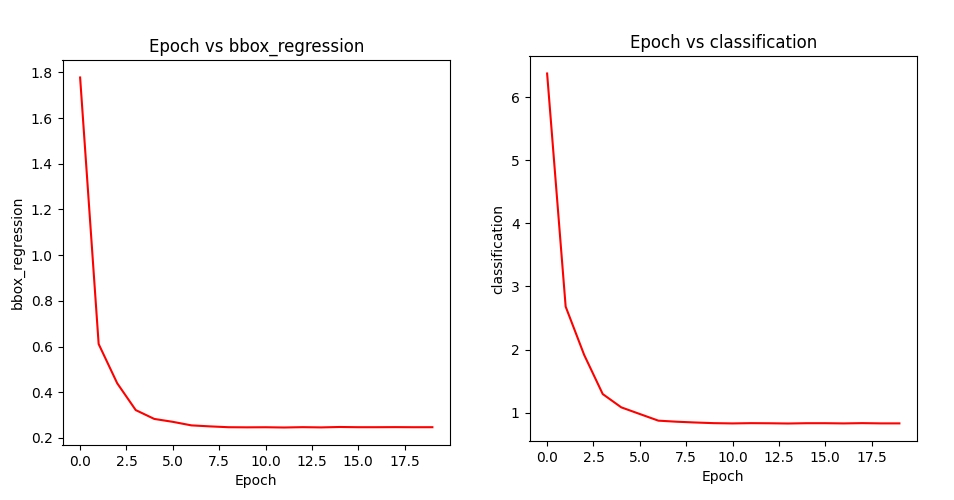
\includegraphics[height=05cm]{ch4-SSD ocr loss.jpg}
	\caption{Courbes de pertes du SSD pour la reconnaissance des chiffres}
\label{fig:ch4-SSD ocr loss}
\end{figure}

\begin{figure}[H]
	\centering
	\includegraphics[height=05cm]{ch4-SSD ocr mAP.jpg}
	\caption{Courbes de mAPs du SSD pour la reconnaissance des chiffres}
\label{fig:ch4-SSD ocr mAP}
\end{figure}

% \textcolor{blue}{Il faut commenter }
%Nous observons que les deux  courbes de perte générées par le modèle SSD pendant l'apprentissage montrent une convergence rapide, nécessitant environ 8 itérations 
%pour atteindre une valeur de perte (loss\_classifier) de prédictions des classes d'objet d'environ 0,5
%pour et une valeur de perte (loss\_box\_reg) approximative de 0.3 pour les prédictions des coordonnées des boites de délimitation.\\
%Comparativement aux courbes de mAP50 et mAP75 d le modèle atteint sa convergence lors de la 15ème itération.À ce stade, les valeurs de mAP50 sont supérieures à 65\%, la mAP75 dépasse les 75\%.

Les courbes de perte du modèle SSD pendant l'apprentissage convergent rapidement, atteignant environ 0,5 pour la perte de classification des classes d'objet et environ 0,3 pour la perte de régression des coordonnées des boîtes de délimitation après environ 8 itérations. En ce qui concerne les courbes de mAP50 et mAP75, le modèle atteint sa convergence à la 15ème itération, avec des valeurs de mAP50 dépassant 65\% et mAP75 dépassant 75\%.

\section{Résultats et discussion}

Dans cette section, nous allons évaluer et comparer les performances de cinq modèles de détection : YOLOv8n, YOLOv8m, YOLOv8s, Faster RCNN et SSD. Nous allons examiner leurs performances tant lors de la phase d'apprentissage que lors des tests pour les tâches de détection des voitures, des plaques d'immatriculation, ainsi que pour la reconnaissance des chiffres d'immatriculation.

L'objectif de cette évaluation est de choisir le modèle le plus performant en vue de son déploiement dans une ordinateur et un smartphone.
% +++++++++++++++++++++++++++++++++++++++++++++++++++++++++++++++++++ result CAR
\subsection{Résultats de l'entraînement et du test des modèles de détection de voitures et de plaques d'immatriculation}

Dans la première expérience, nous faisons varier les valeurs de la dimension de l'image d'entrée et du nombre d'époques d'apprentissage. Nous enregistrons ensuite, pour chaque combinaison de valeurs, la moyenne de la précision moyenne (mAP50), la taille du modèle généré (représentant le fichier de poids résultant de l'apprentissage en MB), et le temps d'apprentissage (en minutes) pour la détection de voitures et de plaques d'immatriculation. Ces résultats sont présentés dans le tableau \ref{table:ch4-training_car_allmodels}.

\begin{table}[h]
	\centering
    \begin{tabular}{|l|l|l|l|l|l|}
    \hline
        Modèle & \shortstack{Dimension \\ d'image}  & Epoque &    mAP50 & \shortstack{Taille \\du modèle}   & \shortstack{Temps\\ d'apprentissage } \\ \hline
        \textbf{YOLOv8n} & \textbf{320x320} &      \textbf{25}     & \textbf{0.995} &  \textbf{6} &      \textbf{38}    \\ \hline
        YOLOv8n &  416x416 &     25     & 0.994  & 6 &     44    \\ \hline
        YOLOv8n & 512x512  &     25    & 0.995   &  6 &  54     \\ \hline
        YOLOv8n & 640x640 &      25     &  0.994    &  6 &   63   \\ \hline
        YOLOv8n & 736x736 &      25     &  0.994  &  6 &       81    \\ \hline
        YOLOv8s & 320x320 &      20      & 0.995  &   6 &     33     \\ \hline
        YOLOv8s & 416x416&       20      & 0.994 &  6 &      38    \\ \hline
        YOLOv8s & 512x512 &       20     &   0.995  &     6 &      48   \\ \hline
        YOLOv8s &  640x640&        20     &  0.995 & 6 &      67     \\ \hline
        YOLOv8s & 736x736  &       20     &   0.995 &   6 &       77   \\ \hline
        YOLOv8m & 320x320  &        20   &  0.996  & 50 &     87     \\ \hline
        SSD     & 320x320  &         10   &  0.984    &   9  &   15   \\ \hline
        Faster R-CNN & 320x320   &   10    &  0.99  &  74 &  17     \\ \hline
    \end{tabular}
    \caption{Performances d'entraînement des modèles de détection de voitures et de plaques}
    \label{table:ch4-training_car_allmodels}
\end{table}
% \textcolor{blue}{A vérifier}
D'après le tableau\ref{table:ch4-training_car_allmodels}, nous observons ce qui suit:\\
- YOLOv8n et YOLOv8s : Ces modèles YOLOv8n et YOLOv8s montrent une performance élevée (mAP50 autour de 0,995) sur différentes dimensions d'images, ce qui indique une capacité de détection précise des objets. Les temps d'apprentissage varient en fonction de la taille de l'image d'entrée, avec des images plus grandes nécessitant plus de temps.\\
- YOLOv8m : Le modèle YOLOv8m atteint une précision légèrement supérieure (mAP50 de 0,996), mais il nécessite un temps d'apprentissage plus long en raison de sa taille plus importante.\\
- SSD : Le modèle SSD montre une performance légèrement inférieure (mAP50 de 0,984) par rapport aux modèles YOLOv8, mais il s'entraîne plus rapidement.\\
- Faster R-CNN : Faster R-CNN atteint une précision élevée (mAP50 de 0,99), mais il nécessite plus de temps d'apprentissage que SSD en raison de sa complexité.

Dans la second expérience, nous avons évalué la vitesse des cinq modèles de détection en termes du temps d'inférence (MS), ainsi que le nombre d'images par seconde (FPS), en tenant compte de la taille de l'image d'entrée, comme présenté dans le tableau \ref{table:ch4-test_speed_car_allmodels}. 
Notre objectif était de sélectionner le modèle qui offre la vitesse de détection la plus élevée pour les voitures et les plaques d'immatriculation tout en maintenant la plus grande précision possible.

\begin{table}[H]
    \centering
    \begin{tabular}{|l|l|l|l|}
    \hline
        Modèle & Dimension d'image & Temps d'inférence & FPS\\ \hline
        \textbf{YOLOv8n} & \textbf{320x320} & \textbf{71} & \textbf{14.1} \\ \hline
        YOLOv8n & 416x416 & 83 & 12.0 \\ \hline
        YOLOv8n & 512x512 & 125 & 8.0 \\ \hline
        YOLOv8n & 640x640 & 167 & 6.0 \\ \hline
        YOLOv8n & 736x736 & 250 & 4.0 \\ \hline
        YOLOv8s & 320x320 & 143 & 7.0 \\ \hline
        YOLOv8s & 416x416 & 200 & 5.0 \\ \hline
        YOLOv8s & 512x512 & 250 & 4.0 \\ \hline
        YOLOv8s & 640x640 & 333 & 3.0 \\ \hline
        YOLOv8s & 736x736 & 500 & 2.0 \\ \hline
        YOLOv8m & 320x320 & 600 & 1.7 \\ \hline
        SSD & 320x320 & 110 & 9.1 \\ \hline
        Faster R-CNN & 320x320 & 600 & 1.7 \\ \hline
    \end{tabular}
    \caption{Comparaison de vitesse d'inférence des modèles de détection de voitures et de plaques }
    \label{table:ch4-test_speed_car_allmodels}
\end{table}

Nous pouvons remarquer, selon le tableau \ref {table:ch4-test_speed_car_allmodels}, que YOLOv8n  semble être le plus rapide parmi les YOLOv8 variantes avec de bonnes performances. Cependant, à mesure que la dimension de l'image augmente, les performances chutent, ce qui est attendu car le modèle doit traiter une image plus grande. YOLOv8s  est plus rapide que YOLOv8n, mais il a également de moins bonnes performances en termes de FPS. Cependant, il offre une meilleure performance par rapport à YOLOv8n pour les images de plus grande dimension. Bien que YOLOv8m ait de bonnes performances en termes de FPS pour des images de petite dimension, il est nettement moins performant que les autres modèles pour des images plus grandes. SSD offre de bonnes performances en termes de FPS pour des images de petite dimension, mais il est moins performant que les modèles YOLO et Faster R-CNN pour des images de plus grande taille. Faster R-CNN est le modèle le plus lent en termes de FPS, mais il offre une performance constante indépendamment de la dimension de l'image.

En conclusion, nous avons opté pour le modèle YOLOv8n, car il a atteint une vitesse de détection élevée avec une taille d'image de 320x320, tout en conservant une précision élevée, affichant un mAP de 0,995. De plus, il a nécessité un temps d'apprentissage modéré et a généré un modèle de petite taille.

En examinant les figures \ref{fig:ch4-test-yolov8-detection-car}, \ref{fig:ch4-test-frcnn-detection-car} et \ref{fig:ch4-test-ssd-detection-car}, nous pouvons constater que le modèle YOLOv8n a obtenu une très bonne détection de véhicules et de plaques d'immatriculation comparée avec les modèles Faster RCNN et SSD. Les boîtes de délimitation sont correctement localisées autour de tous les objets, avec un bon score de prédiction.

\begin{figure}[H]
	\centering
	\includegraphics[height=4cm]{ch4-test-yolov8-detection-car.jpg}
	\caption{Résultats visuels de la détection de voitures et de plaques par YOLOv8n}
 \label{fig:ch4-test-yolov8-detection-car}
\end{figure}

\begin{figure}[H]
	\centering
	\includegraphics[height=04.5cm]{ch4-test-frcnn-detection-car.jpg}
	\caption{Résultats visuels de la détection de voitures et de plaques par Faster R-CNN}
\label{fig:ch4-test-frcnn-detection-car}
\end{figure}

\begin{figure}[H]
	\centering
	\includegraphics[height=04.5cm]{ch4-test-ssd-detection-car.jpg}
	\caption{Résultats visuels de la détection de voitures et de plaques par SSD}
\label{fig:ch4-test-ssd-detection-car}
\end{figure}



% +++++++++++++++++++++++++++++++++++++++++++++++++++++++++++++++++++ result OCR
\subsection{Résultats de l'entraînement et du test des modèles pour le reconnaissance des chiffres}


De manière similaire, nous avons effectué des expériences pour évaluer la reconnaissance des chiffres d'immatriculation. Les résultats de ces expériences sont résumés dans les tableaux \ref{table:ch4-training_ocr_allmodels} et \ref{table:ch4-test_speed_ocr_allmodels}.

\begin{table}[H]
    \centering
    \begin{tabular}{|l|l|l|l|l|l|}
    \hline
        Modèle & \shortstack{Dimension \\d'image } & Epoque &    mAP50 & \shortstack{Taille \\du modèle}   &  \shortstack{Temps \\ d'apprentissage}     \\ \hline
        YOLOv8n & 96x96          &   80         & 0.93   & 6 & 13  \\ \hline
        YOLOv8n & 128x128         &   80       & 0.986   &  6 &  15\\ \hline
        YOLOv8n & 160x160          &   80       & 0.986   &6  & 16 \\ \hline
        YOLOv8n & 192x192         &    80      & 0.986    &6  & 19 \\ \hline
        \textbf{YOLOv8n} & \textbf{224x224} &\textbf{80}& \textbf{0.994}& \textbf{6} &\textbf{20}\\ \hline
        YOLOv8n &  256x256         &   80     & 0.993    & 6 & 20 \\ \hline
        YOLOv8s & 224x224          &   80      & 0.996   & 21 &  20\\ \hline
        YOLOv8m & 320x320          &    20    & 0.996     & 50  & 22 \\ \hline
        SSD      & 320x320         &   40      & 0.96        & 9 & 10 \\ \hline
        Faster R-CNN & 320x320      & 40        & 0.99    & 74 &  20\\ \hline
    \end{tabular}
    \caption{Entraînement des modèles de pour la reconnaissance des chiffres}
    \label{table:ch4-training_ocr_allmodels}
\end{table}

% \textcolor{blue}{Il faut commenter le tableau, quel est le meilleur modèle selon vous, votre interprétation n'est pas complete} 

Selon le tableau \ref{table:ch4-training_ocr_allmodels}), les valeurs de mAP varient de 0,93 à 0,996. Les modèles YOLOv8n, YOLOv8s et YOLOv8m obtiennent une précision élevée dans la reconnaissance des numéros de plaques d'immatriculation, tandis que SSD affiche une précision légèrement inférieure, et Faster R-CNN atteint également une précision importante.

En ce qui concerne le temps d'apprentissage, les modèles ont des temps d'apprentissage similaires, d'environ 20 minutes, à l'exception de YOLOv8m, qui nécessite légèrement plus de temps, soit 22 minutes, et de SSD, qui est encore plus rapide avec seulement 10 minutes.

\begin{table}[H]
    \centering
    \begin{tabular}{|l|l|l|}
    \hline
        Modèle  & Dimension d'image & Temps d'inférence \\ \hline
        YOLOv8n & 96x96& 10 \\ \hline
        YOLOv8n & 128x128 & 10 \\ \hline
        YOLOv8n & 160x160 & 10 \\ \hline
        YOLOv8n & 192x192 & 10 \\ \hline
        \textbf{YOLOv8n} & \textbf{224x224} & \textbf{20} \\ \hline
        YOLOv8n & 256x256 & 30 \\ \hline
        YOLOv8s & 224x224 & 330 \\ \hline
         YOLOv8m & 320x320 & 600 \\ \hline
        SSD & 320 & 110x110 \\ \hline
        Faster R-CNN & 320x320 & 600 \\ \hline
    \end{tabular}
    \caption{Comparaison de vitesse d'inférence des modèles pour la reconnaissance des chiffres}
    \label{table:ch4-test_speed_ocr_allmodels}
\end{table}
% \textcolor{blue}{Il faut commenter le tableau, quel est le meilleur modèle selon vous, votre interprétation n'est pas complete} 

Selon les résultats numériques obtenus et indiqués dans le tableau \ref{table:ch4-test_speed_ocr_allmodels}), les modèles YOLOv8n, YOLOv8s, YOLOv8m, SSD et Faster R-CNN présentent des temps d'inférence variables en fonction de la taille de l'image en entrée. De plus, il est à noter que le modèle YOLOv8n atteint la meilleure mAP, avec une valeur de 0,994, lorsque la taille de l'image d'entrée est réglée à 224.

En ce qui concerne les résultats visuels, les figures \ref{fig:ch4-test-yolov8-detection-ocr}, \ref{fig:ch4-test-frcnn-detection-ocr} et \ref{fig:ch4-test-frcnn-detection-ocr} fournissent une illustration de la reconnaissance des chiffres d’immatriculation par les modèles YOLOv8n, Faster RCNN et SSD. 
Selon ces figures, nous pouvons observer que les boîtes de délimitation prédites par le modèle YOLOv8n ont été générées de manière précise autour de chaque chiffre présent sur les panneaux numériques, avec un taux de prédiction élevé.Entre ce que Faster R-CNN et SSD ont échoué à reconnaître, il y a quelques différences.

\begin{figure}[H]
	\centering
	\includegraphics[height=05cm]{ch4-test-yolov8-detection-ocr.jpg}
	\caption{Résultats visuels de la reconnaissance des chiffres d'immatriculation par YOLOv8n}
\label{fig:ch4-test-yolov8-detection-ocr}
\end{figure}

\begin{figure}[H]
	\centering
	\includegraphics[height=04.5cm]{ch4-test-frcnn-detection-ocr.jpg}
	\caption{ Résultats visuels de la reconnaissance des chiffres par Faster R-CNN}
\label{fig:ch4-test-frcnn-detection-ocr}
\end{figure}


\begin{figure}[H]
	\centering
	\includegraphics[height=05cm]{ch4-test-ssd-detection-ocr.jpg}
	\caption{Résultats visuels de la reconnaissance des chiffres par SSD}
\label{fig:ch4-test-ssd-detection-ocr}
\end{figure}
% +++++++++++++++++++++++++++++++++++++++++++++++++++++++++++++++++++ Comparaison OCR
\subsection{Application des outils spécialisés pour la reconnaissance des chiffres}

En parallèle, nous avons utilisé d'autres outils spécifiques à la reconnaissance ou à la lecture des chiffres d'immatriculation à partir d'images de plaques d'immatriculation, qui contiennent principalement du texte. Parmi ces outils, nous citons notamment EasyOCR\cite{ch4_EasyOCRsdsdsd}, OpenALPR\cite{openalpr-readme} et Tesseract OCR \cite{tesseract-ocr-guide}, en plus des modèles que nous avons développées, en particulier le modèle YOLOv8n.

\textbf{Tesseract OCR :} est un moteur de reconnaissance optique de caractères open source et gratuit, disponible sous licence Apache. Il est développé par Google depuis 2006\cite{ch4_ocr_Tesserac35}. Il est capable de reconnaître des textes imprimés dans une variété de langues, y compris le français, l'anglais, l'allemand, l'espagnol, le chinois et le japonais. Il peut être utilisé pour extraire des textes de documents scannés, de photos et d'autres images. Tesseract est disponible pour les systèmes d'exploitation Windows, macOS et Linux. Il peut être utilisé via une interface de ligne de commande ou une API.

Comme indiqué dans la figure \ref{fig:ch4-tesseract-ocr}, Tesseract n'a pas réussi à reconnaître correctement les chiffres de la plaque d'immatriculation donnée. De plus, sa vitesse de traitement était extrêmement lente.

\begin{figure}[H]
	\centering
	\includegraphics[height=07cm]{ch4-tesseract-ocr.jpg}
	\caption{Reconnaissance des chiffres d'immatriculation à l'aide du Tesseract}
    \label{fig:ch4-tesseract-ocr}
\end{figure}
\textbf{EasyOCR : } est un outil d'OCR gratuit et facile à utiliser. Il peut être utilisé pour extraire des textes de documents scannés, de photos et d'autres images. EasyOCR prend en charge plus de 100 langues et peut reconnaître une variété de formats de texte \cite{ch4_EasyOCRV83}.

Selon la figure \ref{fig:ch4-easyocr}, EasyOCR n'a pas réussi non plus à lire tous les  chiffre de la plaque d'immatriculation testée.

\begin{figure}[H]
	\centering
	\includegraphics[height=07cm]{ch4-easyocr.jpg}
	\caption{Reconnaissance des chiffres d'immatriculation à l'aide du EasyOCR}
    \label{fig:ch4-easyocr}
\end{figure}

\textbf{OpenALPR :} est un outil spécialisé pour la reconnaissance automatique des plaques d'immatriculation. 
Cependant, ces outils présentent certaines limitations. En effet, ils ne sont pas capables de reconnaître certaines plaques d'immatriculation, comme la plaque d'immatriculation algérienne, sans ajustement préalable des paramètres du pays pour l'analyse des images. De plus, ils sont lents et nécessitent un temps de traitement important.

Conformément à ce qui est illustré dans la figure \ref{fig:ch4-openalpr}, lors de l'utilisation d'OpenALPR sur des plaques d'immatriculation américaines, les chiffres sont correctement reconnus, mais cela demande un temps de traitement de 1840 millisecondes. Cependant, lors de son application sur des plaques algériennes, aucun symbole n'est détecté dans la plaque d'immatriculation algérienne, ce qui a été confirmé dans \cite{ch4_OpenALPR81}.
 
\begin{figure}[H]
	\centering
	\includegraphics[height=07cm]{ch4-openalpr.jpg}
	\caption{Reconnaissance des chiffres d'immatriculation à l'aide du OpenALPR}
    \label{fig:ch4-openalpr}
\end{figure}

\section{Gestion de parking : Application pour les véhicules en Algérie}

Dans le cadre de notre projet de fin d'études, nous avons réalisé une application intelligente spécialement conçue pour gérer efficacement le stationnement des conducteurs de véhicules en Algérie.  
Cette application a été développée pour fonctionner sur un ordinateur portable et offre les fonctionnalités suivantes :
\begin{outline}[enumerate]
    \1 Détection des véhicules et des plaques d'immatriculation,
    \1 Reconnaissance des numéros d'immatriculation,
    \1 Suivi en temps réel des véhicules en analysant les vidéos provenant des caméras de surveillance,
    \1 Comptage des véhicules entrants et sortants du parking et l'enregistrement de la date d'entrée ou de sortie des véhicules.
\end{outline} 
La Figure \ref{fig:final_soft} présente l'interface principale de l'application que nous avons développée, où les régions numérotées sont expliquées comme suit :

\begin{figure}[H]
	\centering
	\includegraphics[height=10cm]{ch4-GARIAMAN-001.jpg}
	\caption{Interface graphique de l'application bureautique }
    \label{fig:final_soft}
\end{figure}
\begin{outline}
\1 1. Bouton de démarrage : permet de lancer la lecture de la vidéo à partir des caméras de surveillance.
\1 2. Bouton de pause : permet de figer la vidéo à un instant précis.
\1 3. Bouton d'arrêt : permet d'arrêter la lecture de la vidéo.
\1 4. Taux de rafraîchissement des images par seconde.
\1 5. Boite de délimitation indiquant le véhicule détecté.
\1 6. Boite de délimitation qui encadre la plaque d'immatriculation identifiée.
\1 7. Reconnaissance en temps réel les numéros de plaque d'immatriculation pour le véhicule détecté.
\1 8. Ligne de suivi virtuelle de la voiture avec son identifiant unique.
\1 9. Nombre de véhicule entrant dans le parking.
\1 10. Nombre de véhicule sortant du parking.
\1 11. Liste des numéros de plaques d'immatriculation des voitures entrant dans le parking.
\1 12. Liste des numéros de plaques d'immatriculation des véhicules sortant du parking.
\1 13, 14 et 15 : Ce sont des zones utilisées par l'algorithme de suivi qui a été expliqué dans la sous-section \ref{sec:traking}, où lorsque le point indiqué par la flèche 8 entre dans l'une des zones, le travail se fait comme suit :
       
    \2 Lorsque le point 8 est détecté dans la zone 13, puis quelque temps plus tard, il est détecté dans la zone 15 avec le même identifiant de voiture, le système conclut que la voiture est entrée dans le parking.

    \2 Lorsque le point 8 est détecté dans la zone 15, puis après un certain temps il est détecté dans la zone 13 avec le même identifiant de voiture, le système conclut que la voiture a quitté le parking.

    \2 Lors du passage du Point 8 à la Zone 14, la plaque d'immatriculation de ce véhicule est reconnue sur chaque photo (frame de vidéo ) et enregistrée dans la liste. Lorsque le point 8 quitte la zone 14, le numéro de plaque d'immatriculation le plus courant est envoyé à la base de données avec le statut \{ (Entrée) ou (Sortie) \}, puis la mémoire vive (RAM) sera libérée.
    
\1 Pour ajuster et modifier l'emplacement des zones de capteurs sur l'écran, qui sont constituées des zones 13, 14 et 15, il suffit de sélectionner la zone en cliquant avec le bouton droit de la souris.
   
\end{outline}

Après avoir effectué plusieurs étapes liées à la détection de véhicules, de plaques d'immatriculation et à la reconnaissance des chiffres d'immatriculation, ainsi que le suivi des véhicules, la vitesse de traitement des images a considérablement ralenti. La vitesse de traitement est passée à 10 images par seconde (FPS) en raison du temps nécessaire à la détection des véhicules (71 millisecondes), à la détection des chiffres sur la plaque d'immatriculation (20 millisecondes) et à d'autres tâches de traitement d'image et d'exécution de fonctions supplémentaires. En conséquence, le temps total d'exécution est désormais de 100 millisecondes par image. Pour résoudre ce problème de lenteur, nous envisageons de modifier les outils de développement de l'application  afin de le rendre plus rapide.

\section{Embarquement de l'application de gestion de parking sur les smartphones}

Afin de déployer l'application de gestion de parking pour les véhicules en Algérie sur des appareils mobiles et des puces intégrées, nous avons converti les fichiers de poids résultant de l'entraînement de l'algorithme YOLOV8 en un framework NCNN. Cette étape était essentielle car ces appareils ne prennent généralement pas en charge le langage Python, qui est également moins performant en raison de sa nature interprétée.

Ensuite, nous avons développé une application en \textbf{C++} pour tester et évaluer la vitesse de détection et de reconnaissance à la fois sur un ordinateur portable et un smartphone. Voici les résultats que nous avons obtenus :\\
Sur un ordinateur portable, nous avons atteint les valeurs de FPS suivantes :
\begin{outline}
    \1 27 FPS en utilisant le CPU,
    \1 17 FPS en utilisant le GPU.    
\end{outline}

En ce qui concerne le smartphone, nous avons obtenu les résultats suivants :
\begin{outline}
    \1 25 FPS en utilisant le CPU,
    \1 13 FPS en utilisant le GPU.
\end{outline}

Dans la figure \ref{fig:ch4-application_android}, une capture d'écran de l'interface de l'application mobile est affichée, montrant le résultat de détection de la voiture du test avec sa plaque d'immatriculation. Ce que nous avons remarqué est que la plaque d'immatriculation a été efficacement lue  malgré une vitesse de trame moyenne atteignant 25 images par seconde (FPS).


\begin{figure}[H]
	\centering
	\includegraphics[height=5cm]{ch4-application_android.png}
	\caption{Capture d'écran de l'interface de l'application Android}
    \label{fig:ch4-application_android}
\end{figure}

Il est important de noter que sur un smartphone, la vitesse de rafraîchissement des images (frames) n'est pas constante. Cela est dû au fait que lorsque la température du processeur augmente, le téléphone réduit ses performances.

\section{Problèmes rencontrés et solution adoptées}

Lors du développement des différents modules de l'application, plusieurs problèmes ont été identifiés. Cette section présente les principaux problèmes techniques ainsi que les solutions adoptées.

\textbf{Problème 1:} Une difficulté persistante résidait dans la détection irrégulière des voitures par le modèle YOLO. Dans certaines images, le modèle détectait effectivement une voiture, mais cette détection échouait dans l'image suivante. Cette situation engendrait des interruptions dans la séquence des identifiants de suivi des voitures tout au long de la vidéo.

\textbf{Solution 1:}  Nous avons résolu ce problème en utilisant un filtre de Kalman pour chaque identifiant de voiture. Cette solution permet au système d'estimer la position de la voiture lorsque le détecteur YOLO ne parvient pas à la détecter.

\textbf{Problème 2:}  La lecture répétée des plaques d'immatriculation par notre système à chaque image de la vidéo peut entraîner la répétition de la reconnaissance (lecture) de la même plaque pour une seule voiture, avec parfois des erreurs de reconnaissance.

\textbf{Solution2: }  Pour remédier à cette situation, nous avons mis en place une solution consistant à créer une liste spécifique pour chaque identifiant de voiture. Dans cette liste, nous stockons toutes les plaques d'immatriculation lues pendant le mouvement de la voiture de la zone A à la zone B. Lorsque la voiture quitte la zone B, nous enregistrons les plaques d'immatriculation les plus fréquemment lues dans une base de données. Cette approche contribue à éviter les lectures répétées et à améliorer la fiabilité de la lecture des plaques d'immatriculation.

\section{Conclusion}

Dans ce dernier chapitre, nous avons décrit notre système de gestion de parking pour les véhicules en Algérie. Ce système est capable de détecter les véhicules, les plaques d'immatriculation, de reconnaître les chiffres d'immatriculation et de suivre le mouvement des véhicules entrant et sortant d'un parking. Il repose sur des techniques avancées de vision par ordinateur, en particulier l'apprentissage profond.

Nous avons évalué plusieurs algorithmes de détection d'objets, et à la suite de nombreuses expériences, nous avons choisi YOLOv8n en raison de ses performances exceptionnelles en matière de détection et de reconnaissance. Nous avons également testé divers outils OCR pour la lecture des plaques d'immatriculation. Les résultats obtenus ont montré la supériorité du modèle YOLOv8n dans cette tâche.

%%%%%%%%%%%%pour expliquer le processus de suivi de voiture et de plaque d'immatriculation tout au long de la vidéo, on assignent des identifiants uniques et on analysent leur mouvement pour déterminer leur entrée ou leur sortie du parking.

% Voici une explication générale des étapes mentionnées précédemment:

% \begin{outline}[enumerate]
%     \1 Réception de la vidéo a partir de la caméra de surveillance en temps réel :
%         \2 nous pouvons utiliser la bibliothèque OpenCV pour capturer la vidéo en temps réel à partir de la caméra de surveillance.

%     \1 Détection des voitures et des plaques d'immatriculation à l'aide d'un modèle de détection d'objets :
%        \2 nous pouvons utiliser des modèles tels que Faster R-CNN ou SSD Mobile net v3  ou YOLOV8 pour détecter les voitures dans les images vidéo.
    
%     \1 Découpage de la partie d'image contenant la plaque d'immatriculation :
%        \2 Une fois les voitures et les plaques d'immatriculation détectées, nous pouvons découper la partie de l'image qui contient la plaque d'immatriculation.  en utilisant des bibliothèques de traitement d'image comme OpenCV.
    
%     \1 Extraction du texte (de la plaque d'immatriculation):
%        \2 Pour lire la plaque d'immatriculation, nous pouvons utiliser des algorithmes OCR ou développer un algorithme personnalisé.
    
%     \1 Suivi des voitures dans une vidéo:
%        \2 Il existe plusieurs algorithmes de suivi d'objets que nous pouvons utiliser pour suivre le mouvement des voitures entre les images vidéo consécutives , mais celui qui peut être utilisé dans notre projet est l'algorithme de détection et de suivi (Detection and Tracking) .
    
%     \1 Attribution d'identifiants aux voitures :
%        \2 Lors du suivi des voitures, nous attribuons un identifiant unique à chaque voiture dans la scène, ainsi qu'à sa plaque d'immatriculation.
    
%     \1 Analyse du mouvement des voitures pour déterminer si elles entrent ou sortent du parking :
%        \2 Nous utilisons les identifiants attribués pour analyser le mouvement des voitures, déterminer leur direction et savoir si elles entrent ou sortent du parking.
    
%     \1 Détermination du nombre de voitures entrantes et sortantes du parking :
%         \2 Calcule du nombre de voitures entrantes et sortantes du parking en fonction de l'analyse du mouvement des voitures qui a été effectuée
       
% \end{outline}

% %%%%%%%%%%%%%%%%%%%
% Pour entraîner un modèle de détection d'objets dans des images, plusieurs étapes importantes doivent généralement être suivies:
% \begin{outline}[enumerate]
%     \1 Chargement des bibliothèques : Commençons par charger les bibliothèques de base telles que PyTorch et TorchVision.

%     \1 Sélection et personnalisation du modèle : Choisissons le modèle que nous souhaitons entraîner et personnalisons ses paramètres de base tels que la forme des entrées et des sorties, ainsi que d'autres paramètres selon nos besoins.

%     \1 Création d'une classe pour la lecture des données : Écrivons une classe personnalisée pour lire l'ensemble de données composé d'images et de fichiers de annotations sur les objets, puis convertissons ces données en tensors compréhensibles par le framework.

%     \1 Préparation de données : Au sein de cette étape, redimensionnons les images pour les adapter aux exigences du modèle de détection d'objets et assurons-nous que les données sont correctement formatées, notamment en effectuant le redimensionnement, la normalisation, et l'ajustement des dimensions au besoin.

%     \1 Chargement du modèle : Assurons-nous que le modèle est correctement chargé et converti dans un format compréhensible par le processeur graphique GPU ou l'unité centrale de traitement (CPU).

%     \1 Définition de la fonction de perte : Définissons et choisissons la fonction de perte appropriée à notre tâche .

%     \1 Sélection de l'optimiseur : Choisissons l'optimiseur à utiliser, tel que le SGD (Stochastic Gradient Descent), et configurons ses paramètres, y compris le taux d'apprentissage et le nombre d'étapes.

%     \1 Entraînement du modèle : Effectuons le processus d'entraînement en utilisant une boucle itérative qui comprend les étapes suivantes :
%    \2 Réinitialisation des gradients.
%    \2 Passage en avant (Forward Pass) pour obtenir les prédictions du modèle.
%    \2 Calcul de la perte entre les prédictions et les valeurs réelles.
%    \2 Rétropropagation (Backward Pass) et mise à jour des paramètres du modèle.

%    \1 Sauvegarde du modèle : Après l'entraînement, sauvegardons le modèle pour une utilisation ultérieure sans avoir besoin de le ré-entraîner.

%    \1 Évaluation du modèle : Évaluons les performances du modèle en utilisant des données de test ou de validation pour mesurer son efficacité.

%    \1 Utilisation du modèle : Après avoir réussi l'entraînement, nous pouvons utiliser le modèle pour détecter des objets dans de nouvelles images.

% \end{outline}
\chapter*{Conclusion générale}
\markboth{Conclusion générale}{}
\addcontentsline{toc}{chapter}{Conclusion générale}
\thispagestyle{plain}
% ------------------------------ new 
Ce travail a été développé dans le but de concrétiser notre idée, qui consiste à améliorer l'utilisation des espaces de stationnement grâce à des techniques d'apprentissage profond.

Pour adresser cette problématique, nous avons mis au point un système capable de surveiller les entrées et sorties des véhicules dans le parking, de lire, d'enregistrer et de reconnaître les plaques d'immatriculation. Cette approche nous permet de prédire le nombre de places de stationnement disponibles et de simplifier leur gestion en ayant connaissance des horaires d'arrivée et de départ des véhicules, ainsi que de la durée de chaque opération de stationnement.


Pour accomplir cela, nous avons effectué l'entraînement de modèles de détection d'objets en utilisant deux ensembles de données constitués d'images de voitures algériennes. Le premier ensemble, composé de 2380 images, a été employé pour former un modèle de détection des véhicules et des plaques d'immatriculation algériens. Le second ensemble, comprenant 417 images, a été spécifiquement dédié à la reconnaissance des chiffres présents sur les plaques d'immatriculation algériennes. De plus, nous avons développé un algorithme de suivi du déplacement des véhicules.

Le modèle YOLOv8n\_320 a montré de meilleures performances en termes de précision de détection des véhicules et des plaques d'immatriculation, ainsi qu'en termes de temps d'apprentissage, par rapport aux modèles SSD et Faster R-CNN.

Les travaux menés au cours de ce projet, nous ont permis de percevoir les avantages, et les
limites des techniques élaborées et d'en prévoir des améliorations futures afin de les rendre plus adaptées aux besoins des parkings. Parmi ces améliorations, nous avons l'intention d'enrichir davantage le système en intégrant de nouvelles fonctionnalités, telles que la tarification du stationnement. Un autre domaine d'intérêt pour nous consiste à élargir les bases de données que nous avons crées.

De plus, nous envisageons également le développement d'une application mobile qui permettra aux utilisateurs de localiser le parking le plus approprié en fonction de leurs besoins, tout en fournissant des informations en temps réel sur l'état du stationnement, notamment le nombre de places disponibles et occupées.

% Base de données, fnc
% ------------------------------ old
% \par
% Ce travail a été développé afin de réaliser notre idée qui est un système temps-réel et intelligent pour la gestion de parking, ce système sera capable de prendre en entrée des images des plaques d’immatriculations algériennes et retourne le nombre des places disponible dans le parking.
% \par
% L’objectif de ce projet était d'exploité pleinement l'espace dédié au stationnement, d'accueillir davantage de véhicules, de garantir le confort des conducteurs et de réduire la congestion routière. 
% \par
% Pour remédier à notre problématique, nous avons proposé un système de contrôle qui prend en entré une image de plaque d’immatriculation de la voiture qui entre dans le parking, le système donc va occuper une place, lorsque la voiture sort du parking, le système affiche à l’agent le temps passé par cette véhicule afin de calculer  le montant à payer , et libérer ensuite sa place dans la base de donnée du parking concerné.

% \par
% Afin d’implémenter ce système, nous avons utilisé les réseaux de neurones en utilisant un DataSet que nous avons collecté manuellement contenant 2380 images de plaques d’immatriculations algériennes, nous avons également appuyés sur la technologie d'augmentation de données et l'annotation.
% \par
% Ce travail nous a permis d’approfondir nos connaissances dans le domaine de l’intelligence artificielle en implémentant les modèles d’apprentissage profond à savoir l’algorithme Mask-RCNN utilisé dans l’étape de segmentation Pour celle de la détection, nous avons opté d’implémenter YOLOV8.   
% \par
% Cependant, notre système reste ouvert à des améliorations en perspective, où nous pensons de créer une application Mobile qui montre la localisation des parking les plus proches au chauffeur qui est entrain d’utiliser notre application, et lui est montré le nombre de place disponible dans le parking choisit et le temps en minute entre  le parking et l’endroit ciblé.
% \par


\addcontentsline{toc}{chapter}{Bibliographie}
\lhead{}
\rhead{\textit{Bibliographie}}
\nocite{*}
\bibliographystyle{plain}
\bibliography{biblio}
\end{document}